% arara: makeindex

% Template for IEEE papers
%% bare_conf.tex
%% V1.4b
%% 2015/08/26
%% by Michael Shell
%% See:
%% http://www.michaelshell.org/
%% for current contact information.
%%
%% This is a skeleton file demonstrating the use of IEEEtran.cls
%% (requires IEEEtran.cls version 1.8b or later) with an IEEE
%% conference paper.
%%
%% Support sites:
%% http://www.michaelshell.org/tex/ieeetran/
%% http://www.ctan.org/pkg/ieeetran
%% and
%% http://www.ieee.org/

%%*************************************************************************
%% Legal Notice:
%% This code is offered as-is without any warranty either expressed or
%% implied; without even the implied warranty of MERCHANTABILITY or
%% FITNESS FOR A PARTICULAR PURPOSE!
%% User assumes all risk.
%% In no event shall the IEEE or any contributor to this code be liable for
%% any damages or losses, including, but not limited to, incidental,
%% consequential, or any other damages, resulting from the use or misuse
%% of any information contained here.
%%
%% All comments are the opinions of their respective authors and are not
%% necessarily endorsed by the IEEE.
%%
%% This work is distributed under the LaTeX Project Public License (LPPL)
%% ( http://www.latex-project.org/ ) version 1.3, and may be freely used,
%% distributed and modified. A copy of the LPPL, version 1.3, is included
%% in the base LaTeX documentation of all distributions of LaTeX released
%% 2003/12/01 or later.
%% Retain all contribution notices and credits.
%% ** Modified files should be clearly indicated as such, including  **
%% ** renaming them and changing author support contact information. **
%%*************************************************************************


% *** Authors should verify (and, if needed, correct) their LaTeX system  ***
% *** with the testflow diagnostic prior to trusting their LaTeX platform ***
% *** with production work. The IEEE's font choices and paper sizes can   ***
% *** trigger bugs that do not appear when using other class files.       ***                          ***
% The testflow support page is at:
% http://www.michaelshell.org/tex/testflow/

\documentclass{book}
\usepackage[quiet]{fontspec}
\usepackage[table,xcdraw,dvipsnames]{xcolor} % Used by spritegrid and others.
\usepackage[obeyspaces,spaces]{url}
\usepackage{longtable}
\usepackage{arydshln}
\usepackage{booktabs}
\usepackage{afterpage}
\usepackage{flushend}
\usepackage{titletoc}
\usepackage[toc]{appendix}
\usepackage{parskip}
\usepackage{graphicx,wrapfig}
\usepackage{float}
\usepackage{caption}
\usepackage{pdfpages}
\usepackage{tikzpagenodes}
\usepackage{imakeidx}
\usepackage[pagestyles,raggedright]{titlesec}
\usepackage[all]{nowidow}
\usepackage[bookmarks=true,linktoc=all]{hyperref}
\hypersetup{
  colorlinks   = true, %Colours links instead of ugly boxes
  urlcolor     = blue, %Colour for external hyperlinks
  % Each main .tex file configures via \titleformat the \chapter command
  % to do {\chapmtoc\insertminitoc} and \chapmtoc, as defined below, will
  % use \hypersetup{linkcolor=white} to avoid blue-on-blue TOC links
  % Besides, each main .tex file will issue the \tableofcontents command
  % between \hypersetup{linkcolor=black} and \hypersetup{linkcolor=blue}
  % This means however that if "blue" is modified here it must be modified
  % in these files too.
  linkcolor    = blue, %Colour of internal links
  citecolor   = red %Colour of citations
}
\usepackage{aeb-minitoc}
\usepackage{fix-cm}
\usepackage{textpos}
\usepackage{enumitem}
\usepackage{tcolorbox}
\tcbuselibrary{breakable,listings,skins,xparse}
%\usepackage{wrapfig}
\usepackage{needspace}
\usepackage{verbatim}
\usepackage{ean13isbn}
\usepackage{setspace}

% Use CHAPTER-PAGE page numbering to make it easier to modify chapters
% later, without messing up page number of the rest of the book.
\usepackage[auto]{chappg}

% Allow cross-references between the various books to the big The MEGA65 Book
\usepackage{xr}
\usepackage{varioref}
\usepackage{xparse}
\externaldocument[M65Book-]{mega65-book}
% And a \ref alternative that checks if it needs to be a cross-reference to the
% MEGA65 Book instead.
\makeatletter
\newcommand{\bookref}[1]{%
    \@ifundefined{r@#1}{%
      {\em the MEGA65 Book}, \nameref{M65Book-#1} (\autoref{M65Book-#1})}{\autoref{#1}}%
}
\newcommand{\bookvref}[1]{%
    \@ifundefined{r@#1}{%
      {\em the MEGA65 Book}, \nameref{M65Book-#1} (\autoref{M65Book-#1})}{Chapter/Appendix \vref{#1}}%
}
\makeatother

% For fixed-width columns in register maps
\usepackage{array}

% Makes tables with double-ruled lines look better
\usepackage{hhline}

% Makes better use of space for reference tables in appendix
\usepackage{multicol}

% Shaded tables with alternate rows colored for better legibility
% Best used with larger tables rather than small tables
\usepackage{colortbl}
\usepackage{adjustbox}
\usepackage[strict]{changepage}

% \makecell command for forcing line breaks in table cells
\usepackage{makecell}

\newcolumntype{L}[1]{>{\raggedright\let\newline\\\arraybackslash\hspace{0pt}}m{#1}}
\newcolumntype{C}[1]{>{\centering\let\newline\\\arraybackslash\hspace{0pt}}m{#1}}
\newcolumntype{R}[1]{>{\raggedleft\let\newline\\\arraybackslash\hspace{0pt}}m{#1}}

% clear to left page for making two page tables starting on the odd page
\newcommand{\cleartoleftpage}{%
  \clearpage
  \ifodd\value{page}\hbox{}\newpage\fi
}

% For displaying Letter keys and the MEGA key
% This is a `keys' element for displaying a Mega65 keyboard key
% using a black filled label with rounded edges.
% In order to display a key as a title, use:
%
%     \megakey[title]{Run/Stop}
%
% For displaying a key as a part of the normal document flow, simply use:
%
%    \specialkey{SHIFT}
%
%
% If you get warnings on special characters, mathematical characters etc, use $, eg:
%
%    \megakey{$\leftarrow$}
%
% Other sizes are supported, as part of tcolorbox:
% http://mirror.aarnet.edu.au/pub/CTAN/macros/latex/contrib/tcolorbox/tcolorbox.pdf#subsubsection.4.7.5 however, only `title' and the default: `small' are proposed for use in this manual.
%
% The second macro available here is the megasymbolkey.
% This will display the MEGA symbol as white on a black key box. Simply use:
%
%		 \megasymbolkey
%
% Some MEGA65 keys contain two lines of text like "RUN/STOP"
% You can use the specialkey macro for this:
%
%    \specialkey{SHIFT LOCK}%

\usepackage{tcolorbox}

\newtcbox{\megakeyinner}[1][small]{colback=black, coltext=white, size=#1, fontupper=\bfseries, nobeforeafter,box align=bottom,baseline=3pt,text height=7pt,valign=center}
\newcommand{\megakey}[2][small]{\megakeyinner[#1]{\uppercase{#2}}}

\newtcbox{\megakeyinnerwhite}[1][small]{colback=white, coltext=black, size=#1, fontupper=\bfseries, nobeforeafter,box align=bottom,baseline=3pt,text height=7pt,valign=center}
\newcommand{\megakeywhite}[2][small]{\megakeyinnerwhite[#1]{\uppercase{#2}}}

% Previous version of megasymbolkey
%\newtcbox{\megasymbolkeyinner}{colback=black, coltext=white, clip title=false. fontupper=\symbolfont, box align=bottom,baseline=3pt,text height=7pt}
%\newcommand{\megasymbolkey}{\megakeyinner{\megasymbol[white]}\ }

\newtcolorbox{megasymbolkeyinner}
{colback=black,coltext=white,size=small,fontupper=\small\bfseries,
width=0.65cm, height=0.55cm, box align=base,
nobeforeafter, halign=flush left, left=0mm,top=0.3mm,bottom=0mm,right=0mm
,boxsep=0.5mm,baseline=4pt, enlarge right by = 1mm
}
\newcommand{\megasymbolkey}{
\begin{megasymbolkeyinner}%
\megasymbol[white]%
\end{megasymbolkeyinner}%
}

\newtcolorbox{specialkeyinner}
{colback=black,coltext=white,size=small,fontupper=\tiny\bfseries,
width=0.80cm, height=0.55cm, box align=base,
nobeforeafter, halign=flush left, left=0mm,top=0.3mm,bottom=0mm,right=0mm
,boxsep=0.5mm,baseline=4pt
}
\newcommand{\specialkey}[1]{
\begin{specialkeyinner}%
#1%
\end{specialkeyinner}%
}

\newtcolorbox{widekeyinner}
{colback=black,coltext=white,size=small,fontupper=\tiny\bfseries,
width=0.9cm, height=0.55cm, box align=base,
nobeforeafter, halign=flush left, left=0mm,top=0.3mm,bottom=0mm,right=0mm
,boxsep=0.5mm,baseline=4pt
}
\newcommand{\widekey}[1]{
\begin{widekeyinner}%
#1%
\end{widekeyinner}%
}




% For displaying print versions petscii character symbols
\input{elements/graphicsymbol}

% For Mega65 display of code, listings and screen activity
% This is a collection of elements for displaying output from the Mega65 screen.
% They can display program code or fragments to show activity on the screen.
% Example of use:
%
%    \begin{screencode}
%    10 OPEN 1,8,0,"$0:*,P,R
%    20 : IF DS THEN PRINT DS$: GOTO 100
%    30 GET#1,X$,X$
%    40 DO
%    50 : GET#1,X$,X$: IF ST THEN EXIT
%    60 : GET#1,BL$,BH$
%    70 : LINE INPUT#1, F$
%    80 : PRINT LEFT$(F$,18)
%    90 LOOP
%    100 CLOSE 1
%
%    RUN
%    \end{screencode}
%
% for inline display of code, use:
%
%    \screentext{?SYNTAX ERROR}
%

\usepackage{listings,color}

\lstnewenvironment{screenoutputlined}
   {
     \lstset{
               basicstyle=\codefont\color{white}\linespread{1.0}\normalsize,
               backgroundcolor=\color{black},fillcolor=\color{black},
               rulecolor=\color{black},
               frame=lines,
               framexleftmargin=2mm,
               framexrightmargin=2mm,
               framextopmargin=2mm,
               framexbottommargin=2mm,
               tabsize=4,
               xleftmargin=2mm,
               xrightmargin=2mm,
               basewidth={0.4em},
               literate={\*}{*}1{\-}{-}1{\/}{/}1{{\ }}{{ }}1
            }
   }
   {  }

\lstdefinestyle{megalisting}{basicstyle=\codefont\normalsize,breaklines=false,fontadjust=true,basewidth=1.5mm}
\makeatletter
\newtcblisting{screencode}{%
listing only,
colback=black,
coltext=white,
boxsep=0mm,
left=2mm,
right=0mm,
top=-1mm,
bottom=-1mm,
listing options={style=megalisting},
% Gets ignored by listings package
%fontupper=,
%enlarge left by =\csname @totalleftmargin\endcsname
}
\makeatother

% Stop - signs in listings getting turned into minus characters
\makeatletter
\lst@CCPutMacro
    \lst@ProcessOther {"2D}{\lst@ttfamily{-{}}{-}}
    \@empty\z@\@empty
% Also stop * being pushed down or faultily verically centred
\lst@CCPutMacro
    \lst@ProcessOther {"2A}{%
      \lst@ttfamily
         {{*}}% used with ttfamily
         {*}}% used with other fonts
    \@empty\z@\@empty
\makeatother


% For in-line screen text
\newcommand{\screentext}[1]{{\codefont\color{black}\normalsize{#1}}}
\newcommand{\screentextwide}[1]{{\codefontwide\color{black}\small{#1}}}
% Just to save typing
\newcommand{\stw}[1]{{\codefontwide\color{black}\small{#1}}}

% 45GS02 assembler mneomics and Acme directives
\lstdefinelanguage[45gs02]{Assembler}%
  {morekeywords={%
    adc,and,asl,asr,asw,aug,bbr0,bbr1,bbr2,%
    bbr3,bbr4,bbr5,bbr6,bbr7,bbs0,bbs1,bbs2,%
    bbs3,bbs4,bbs5,bbs6,bbs7,bcc,bcs,beq,%
    bit,bmi,bne,bpl,bra,brk,bsr,bvc,%
    bvs,clc,cld,cle,cli,clv,cmp,cpx,%
    cpy,cpz,dec,dew,dex,dey,dez,eom,%
    eor,inc,inw,inx,iny,inz,jmp,jsr,%
    lda,ldx,ldy,ldz,lsr,map,neg,nop,%
    ora,pha,php,phw,phx,phy,phz,pla,%
    plp,plx,ply,plz,rmb0,rmb1,rmb2,rmb3,%
    rmb4,rmb5,rmb6,rmb7,rol,ror,row,rti,%
    rts,sbc,sec,sed,see,sei,smb0,smb1,%
    smb2,smb3,smb4,smb5,smb6,smb7,sta,stx,%
    sty,stz,tab,tax,tay,taz,tba,trb,%
    tsb,tsx,tsy,txa,txs,tya,tys,tza,%
    adcq,andq,aslq,asrq,bitq,cmpq,deq,eorq,%
    inq,ldq,lsrq,orq,rolq,rorq,sbcq,stq},%
  morekeywords=[2]{%
    !8,!08,!by,!byte,!16,!wo,!word,!le16,%
    !be16,!24,!le24,!be24,!32,!le32,!be32,!hex,%
    !h,!fill,!fi,!skip,!align,!convtab,!ct,!text,%
    !tx,!pet,!raw,!scr,!scrxor,!to,!source,!src,%
    !binary,!bin,!zone,!zn,!symbollist,!sl,!if,!ifdef,%
    !ifndef,!for,!set,!do,!while,!endoffile,!eof,!warn,%
    !error,!serious,!macro,!initmem,!xor,!pseudopc,!cpu,!al,!as,!rl,!rs,!address,!addr,
  },%
  alsoletter=.,%
  alsodigit=?,%
  sensitive=f,%
  morestring=[b]",%
  morestring=[b]',%
  morecomment=[l]{;}%
  }[keywords,comments,strings]

\lstdefinelanguage[MEGA65]{Basic}%
  {morekeywords={%
    end,for,next,data,input\#,input,dim,read,%
    let,goto,run,if,restore,gosub,return,rem,%
    stop,on,wait,load,save,verify,def,poke,%
    print\#,print,cont,list,clr,cmd,sys,open,%
    close,get,new,tab,to,fn,spc,then,%
    not,step,+,-,*,/,\^,and,%
    or,>,=,<,sgn,int,abs,usr,%
    fre,pos,sqr,rnd,log,exp,cos,sin,%
    tan,atn,peek,len,str\$,val,asc,chr\$,%
    left\$,right\$,mid\$,go,rgraphic,rcolor,joy,rpen,%
    dec,hex\$,err\$,instr,else,resume,trap,tron,%
    troff,sound,vol,auto,import,graphic,paint,char,%
    box,circle,paste,cut,line,merge,color,scnclr,%
    xor,help,do,loop,exit,dir,dsave,dload,%
    header,scratch,collect,copy,rename,backup,delete,renumber,%
    key,monitor,using,until,while,bank,filter,play,%
    tempo,movspr,sprite,sprcolor,rreg,envelope,sleep,catalog,%
    dopen,append,dclose,bsave,bload,record,concat,dverify,%
    dclear,sprsav,collision,begin,bend,window,boot,fread\#,%
    wpoke,fwrite\#,dma,edma,mem,off,fast,speed,%
    type,bverify,ectory,erase,find,change,set,screen,%
    polygon,ellipse,viewport,gcopy,pen,palette,dmode,dpat,%
    format,turbo,foreground,background,border,highlight,mouse,rmouse,%
    disk,cursor,rcursor,loadiff,saveiff,edit,font,fgoto,%
    fgosub,mount,freezer,chdir,dot,info,bit,unlock,%
    lock,mkdir,<<,>>,vsync,pot,bump,%
    lpen,rsppos,rsprite,rspcolor,log10,rwindow,pointer,mod,%
    pixel,rpalette,rspeed,rplay,wpeek,decbin,strbin\$%
  },%
  sensitive=f,%
  morestring=[b]",%
  morecomment=[l]{rem }%
  }[keywords,comments,strings]

\lstnewenvironment{asmcode}{
  \lstset{
    language=[45gs02]Assembler,
    basicstyle=\ttfamily\normalsize,
    xleftmargin=4mm}
}{}
\newcommand\asminput[2][]{%
  \lstinputlisting[
    language=[45gs02]Assembler,
    basicstyle=\ttfamily\normalsize,
    xleftmargin=4mm,
    #1]{#2}
}

\lstnewenvironment{basiccode}{
  \lstset{
    language=[MEGA65]Basic,
    basicstyle=\ttfamily\normalsize,
    xleftmargin=4mm}
}{}
\newcommand\basicinput[2][]{%
  \lstinputlisting[
    language=[MEGA65]Basic,
    basicstyle=\ttfamily\normalsize,
    xleftmargin=4mm,
    #1]{#2}
}


% For MEGA65 screen shots with text flow
\input{elements/screenshots}

% For displaying sprite data in a grid
\input{elements/spritegrid}

% Don't number sections
\setcounter{secnumdepth}{0}

\renewcommand{\indexname}{INDEX}
\renewcommand{\appendixtocname}{APPENDICES}
\renewcommand{\appendixpagename}{APPENDICES}
\renewcommand{\appendixpage}{%
  \clearpage\thispagestyle{empty}
    \pagecolor{blue}
     \begin{center}
       {
         \large
         % Put a nice amount of vertical space before the title
         \vspace*{2cm}
               {\large\Huge\textcolor{white}{\bf{APPENDICES}}}\\
             \vspace{\fill}
       }
     \end{center}
     \newpage\pagecolor{white}\clearpage
}

\makeatletter\chardef\pdf@shellescape=\@ne\makeatother

\setcounter{tocdepth}{5}

% 1.0 cm is the distance from left of page to bullet point.
% 2.8 cm is a fudge-factor to make multi-line section names be correctly lined up.
% \@B{〈length〉} is the amount to indent prior to〈sec-num >
% \@F{〈fmt〉} is the formatting for the title heading
% \@P{〈fmt〉} is the formatting for the page number (〈pg-num〉).

\TOCLevels{chapter}{section}
\begin{minitocfmt}{\chapmtoc}
\declaretocfmt{section}{\@F{\color{white}\hypersetup{linkcolor=white}\hspace{1.0cm}\textbullet\hspace{0.25cm}\Large\bfseries}\@B{2.8cm}\@P{\mtocgobble}}
\declaretocfmt{section*}{\@F{\color{white}\hypersetup{linkcolor=white}\hspace{1.0cm}\textbullet\hspace{0.25cm}\Large\bfseries}\@B{2.8cm}\@P{\mtocgobble}}
\end{minitocfmt}

\usepackage{fontspec}
\usepackage{courier}

\setmainfont[Path=fonts/, BoldFont=MegaGlacial-Bold.otf, ItalicFont=MegaGlacial-Italic.otf]{MegaGlacial-Regular.otf}
\setmonofont[Path=fonts/, BoldFont=Inconsolata-Bold.ttf]{Inconsolata-Regular.ttf}
\newfontfamily\serifed[Path=fonts/, BoldFont=xits-bold.otf, ItalicFont=xits-italic.otf]{xits-regular.otf}
\newfontface\codefont[Path=fonts/, ItalicFont=mega80-Reverse.ttf]{mega80-Regular.ttf}
\newfontface\codefontwide[Path=fonts/]{mega40-Regular.ttf}
\newfontface\symbolfont[Path=fonts/]{MEGA65GraphicSymbols.otf}


% Set margins for inner and outer pages in A5 book format
\ifdefined\printmanual
\usepackage[a5paper,nomarginpar,includemp,bottom=2cm,top=1cm,inner=1.8cm,outer=0.8cm, footskip = 1cm]{geometry}
\else
\usepackage[a5paper,nomarginpar,includemp,bottom=2cm,top=1cm,inner=1.0cm,outer=1.0cm, footskip = 1cm]{geometry}
\fi

% Some Computer Society conferences also require the compsoc mode option,
% but others use the standard conference format.
%
% If IEEEtran.cls has not been installed into the LaTeX system files,
% manually specify the path to it like:
% \documentclass[conference]{../sty/IEEEtran}

%% \input{setup}

% correct bad hyphenation here
\hyphenation{op-tical net-works semi-conduc-tor}

\makeindex[intoc]

\pagestyle{empty}

\begin{document}
\raggedbottom

% relax word wrapping with sloppy
\sloppy
% reduce overfull \hbox warnings
\hfuzz=5pt

% macro for changing the verbatim font
\makeatletter
\newcommand{\verbatimfont}[1]{\def\verbatim@font{#1}}%
\makeatother



%\pagecolor{blue}
%\clearpage\thispagestyle{empty}
%\begin{center}
%
\includegraphics[width=\textwidth]{frontcover/MEGA65_logo_shadow}
%
%{\textcolor{white}{\large\Huge{\bf{USER'S GUIDE}}}}
%
%\vspace{\fill}
%\end{center}
%
\newcommand\titlestreq[3]{%
  \IfStrEq{#1}{\detokenize{#2}}{\includegraphics[height=210mm,width=149mm]{\detokenize{#3}}}{}%
}

\newcommand\titlepic[1]{%
  \titlestreq{#1}{mega65-book}{frontcover/m65book\_title}%
  \titlestreq{#1}{mega65-userguide}{frontcover/userguide\_title}%
  \titlestreq{#1}{mega65-developer-guide}{frontcover/developer\_title}%
  \titlestreq{#1}{mega65-chipset-reference}{frontcover/chipset\_title}%
  \titlestreq{#1}{mega65-basic65-reference}{frontcover/basic65\_title}%
}

\begin{tikzpicture}[remember picture,overlay,shift={(current page.north east)}]
\node[anchor=north east,xshift=0.2cm,yshift=0.1cm]{\titlepic{\jobname}};
\end{tikzpicture}

%\newpage
%\pagecolor{white}

%\vspace*{-2cm}\chapter*{MEGA65 TEAM}
\newpage
{\huge MEGA65 TEAM}\vspace{1cm}

\begin{mega65thanks}

\begin{minipage}{\linewidth}
    {\large\bf Dr. Paul Gardner-Stephen} \\
    \textit{(highlander)} \\
    Founder \\
    Software and virtual hardware architect \\
    Spokesman and lead scientist
\end{minipage}

\begin{minipage}{\linewidth}
    {\large\bf Martin Streit} \\
    \textit{(seriously)} \\
    Video and photo production \\
    Tax and organization \\
    Social media
\end{minipage}

\begin{minipage}{\linewidth}
    {\large\bf Dan Sanderson} \\
    \textit{(dddaaannn)} \\
    Media and documentation \\
    MEGA65.ROM
\end{minipage}

\begin{minipage}{\linewidth}
    {\large\bf Dr. Edilbert Kirk} \\
    \textit{(Bit Shifter)} \\
    MEGA65.ROM \\
    Manual and tools
\end{minipage}

\begin{minipage}{\linewidth}
    {\large\bf Gábor Lénárt} \\
    \textit{(LGB)} \\
    Emulator
\end{minipage}

\begin{minipage}{\linewidth}
    {\large\bf Farai Aschwanden} \\
    \textit{(Tayger)} \\
    Filehost and tools \\
    Financial advisory
\end{minipage}

\begin{minipage}{\linewidth}
    {\large\bf Falk Rehwagen} \\
    \textit{(bluewaysw)} \\
    GEOS
\end{minipage}

\begin{minipage}{\linewidth}
    {\large\bf Robert Steffens} \\
    \textit{(kibo)} \\
    Network technology \\
    Core bug hunting
\end{minipage}

\begin{minipage}{\linewidth}
    {\large\bf Detlef Hastik} \\
    \textit{(deft)} \\
    Co-founder \\
    General manager \\
    Marketing and sales
\end{minipage}

\begin{minipage}{\linewidth}
    {\large\bf Oliver Graf} \\
    \textit{(lydon)} \\
    Release management \\
    VHDL and platform enhancements
\end{minipage}

\begin{minipage}{\linewidth}
    {\large\bf Antti Lukats} \\
    \textit{(antti-brain)} \\
    Host hardware design and production
\end{minipage}

\begin{minipage}{\linewidth}
    {\large\bf Dieter Penner} \\
    \textit{(doubleflash)} \\
    Host hardware support
\end{minipage}

\begin{minipage}{\linewidth}
    {\large\bf Mirko H.} \\
    \textit{(sy2002)} \\
    Additional platforms and consulting
\end{minipage}

\begin{minipage}{\linewidth}
    {\large\bf Gürçe Işıkyıldız} \\
    \textit{(gurce)} \\
    Tools and enhancements
\end{minipage}

\begin{minipage}{\linewidth}
    {\large\bf Daniel England} \\
    \textit{(Mew Pokémon)} \\
    Additional code and tools
\end{minipage}

\begin{minipage}{\linewidth}
    {\large\bf Hernán Di Pietro} \\
    \textit{(indiocolifa)} \\
    Additional emulation and tools
\end{minipage}

\begin{minipage}{\linewidth}
    {\large\bf Roman Standzikowski} \\
    \textit{(FeralChild)} \\
    Open ROMs
\end{minipage}

\begin{minipage}{\linewidth}
    {\large\bf Anton Schneider-Michallek} \\
    \textit{(adtbm)} \\
    Presentation and support
\end{minipage}

\end{mega65thanks}

\newpage
{\huge Reporting Errors and Omissions}\vspace{1cm}

This book is being continuously refined and improved upon by the MEGA65 community.
The version of this edition is:

\input{gitinfo}

We want this book to be the best that it possibly can. So if you see any errors,
find anything that is missing, or would like more information,
please report them using the MEGA65 User's Guide issue tracker:

\url{https://github.com/mega65/mega65-user-guide/issues}

You can also check there to see if anyone else has reported a similar problem,
while you wait for this book to be updated.

Finally, you can always download the latest versions of our suite of books from these locations:

\begin{itemize}
\item \url{https://mega65.org/mega65-book}
\item \url{https://mega65.org/user-guide}
\item \url{https://mega65.org/developer-guide}
\item \url{https://mega65.org/basic65-ref}
\item \url{https://mega65.org/chipset-ref}
\item \url{https://mega65.org/docs}
\end{itemize}


%
% paper title
% Titles are generally capitalised except for words such as a, an, and, as,
% at, but, by, for, in, nor, of, on, or, the, to and up, which are usually
% not capitalised unless they are the first or last word of the title.
% Linebreaks \\ can be used within to get better formatting as desired.
% Do not put math or special symbols in the title.

\cleardoublepage

\pagenumbering{roman}

  \begin{titlepage}
    \pagecolor{blue}
     \begin{center}
       {
         \large
         % Put a nice amount of vertical space before the title
         \vspace*{2cm}
               {\Huge\textcolor{white}{\bf{MEGA65 REFERENCE GUIDE}}}\\
             \vspace{\fill}
                    {\textcolor{white}{Published by \\ the MEGA Museum of Electronic Games \& Art e.V., Germany.}}
       }
     \end{center}
   \end{titlepage}

% Then the copyright notice page
  \pagecolor{white}\textcolor{black}
  \vfill
  WORK IN PROGRESS

  \index{copyright}Copyright \copyright 2018 -- 2023 by Paul Gardner-Stephen, the MEGA Museum of Electronic Games \& Art e.V., and contributors.

  This reference guide is made available under the GNU Free Documentation License v1.3, or later, if desired. This means that you are free to modify, reproduce
  and redistribute this reference guide, subject to certain conditions. The full text of the GNU Free Documentation License v1.3 can be
  found at \url{https://www.gnu.org/licenses/fdl-1.3.en.html}.

  Implicit in this copyright license, is the permission to duplicate and/or redistribute this document in whole or in part for use in
  education environments.  We want to support the education of future generations, so if you have any worries or concerns, please
  contact us.

   \par\today

\newpagestyle{onlynumber}{\setfoot[][{\bf\small\thepage}][]
                                  {} {\bf\small\thepage} {}}
\pagestyle{onlynumber}
\pagecolor{white}

\hypersetup{linkcolor=black}
\tableofcontents
\hypersetup{linkcolor=blue}

%% XXX - big numbers are not in bold, because latex gets confused
\newcommand*{\justifyheading}{\raggedleft}
\definecolor{headingblue}{rgb}{0.5,0.5,1}

% \titleformat{command}[shape]
%   {format}
%   {label}
%   {sep}
%   {before}
%   [after]

% ***************
% PART title page
% ***************

\titleclass{\part}{top}
\titleformat{\part}[display]
   {\thispagestyle{empty}\pagecolor{blue}\normalfont\huge\bfseries\justifyheading}
   {\textcolor{white}{\fontsize{50}{65}\selectfont\bf{PART}\quad{\fontsize{100}{130}\selectfont \bf{\serifed\thepart}}}}
   {20pt}
   {\Huge\textcolor{white}}
   [\newpage\pagecolor{white}\textcolor{black}]

% ******************
% CHAPTER title page
% ******************

\titleformat{\chapter}[display]
   {\thispagestyle{empty}\pagecolor{blue}\normalfont\huge\bfseries\justifyheading}
   {\textcolor{white}{\MakeUppercase{\chaptertitlename}\quad{\fontsize{100}{130}\selectfont \bf\thechapter}}}
   {20pt}
   {\Huge\textcolor{white}}
   [{\chapmtoc\insertminitoc}\newpage\pagecolor{white}\textcolor{black}\cleardoublepage]

% ******************
% SECTION title page
% ******************

\titleformat{\section}[display]
   {\raggedright}
   {\thesection}
   {20pt}
   {\huge\bf\color{headingblue}\uppercase}
   [\color{black}]

%\titlecontents{\chapter}

\cleardoublepage
\pagenumbering{arabic}


\part{APPENDICES}

\appendix
  \input{appendix-mathfunctions}
  \input{appendix-pinouts}
  \chapter{45GS02 Microprocessor}
\label{cha:cpu}
\label{cha:45gs02}
\section{Introduction}

The 45GS02 is an enhanced version of the processor portion of the CSG4510
and of the F018 "DMAgic" DMA controller used in the Commodore 65
computer prototypes.  The 4510 is, in turn,
an enhanced version of the 65CE02.
The reader is referred to
the considerable documentation available for the 6502 and 65CE02 processors
for the backwards-compatible operation of the 45GS02.

This chapter will
focus on the differences between the 45GS02 and the earlier 6502-class
processors, and the documentation of the many built-in memory-mapped I/O
registers of the 45GS02.

\section{Differences to the 6502}

The 45GS02 has a number of key differences to earlier 6502-class processors:

\subsection{Supervisor/Hypervisor Privileged Mode}

Unlike the earlier 6502 variants, the 45GS02 has a privileged mode of operation.
This mode is intended for use by an operating system or type-1
hypervisor.  The ambiguity between
operating system and Hypervisor on the MEGA65 stems from the fact that the operating
system of the MEGA65 is effectively little more than a loader and
task-switcher for C64 and C65
environments, i.e., effectively operating as a hypervisor, but provides
only limited virtualisation
of the hardware.

The key differences between normal and supervisor mode on the MEGA65, are that in
supervisor mode:

\begin{itemize}
\item A special 16KB memory area is mapped to \$8000 - \$BFFF, which is
 used to contain both
 the program and data of the Hypervisor / supervisor program.
 This is normally the Hyppo program.
  This memory is not mappable by any means when the processor is in the
 normal mode (the chip-select
  line to it is inhibited), protecting it from accidental or malicious access.
\item The 64 SYSCALL trap registers in the MEGA65 I/O-mode at
\$D640 - \$D67F are replaced by the
  virtualisation control registers.  These registers allow complete
control over the system, and
  it is their access that truly defines the privilege of the supervisor mode.
  \item The processor always operates at full speed (40MHz) and in the
 4510 processor personality.
\end{itemize}

The Hypervisor Mode is described in more detail later in this appendix.

\subsection{6502 Unintended Instructions}

The 65C02, 65CE02 and CSG4510 processors extended the original 6502 processor
by using previously unallocated opcodes of the 6502 to provide additional
instructions.  All software that followed the official documentation of the 6502
processor will therefore work on these newer processors, possibly with different
instruction timing.  However, the common practice on the C64 and other home computers
of using undefined or unintended opcodes (often called ``illegal opcodes'', although
there is no law against using them), means that many existing programs will not work
on these newer processors.

To alleviate this problem the 45GS02 has the ability to switch processor personalities
between the 4510 and 6502.  The effect is that in 6502 mode, none of the new opcodes of
the 65C02, 65CE02, 4510 or 45GS02 are available, and are replaced with the original,
often strange, behaviour of the undefined opcodes of the 6502.

\begin{quote}
{\bf WARNING:} This feature is incomplete and untested.  Most unintended
6502 instructions do not operate correctly when the 6502 personality is enabled.
\end{quote}

\subsection{Read-Modify-Write Instruction Bug Compatibility}

The 65CE02 processor optimised a group of instructions called the
Read-Modify-Write (RMW) instructions.  For such instructions, such as
INC, that increments the contents of a memory location, the 6502 would
read the original value and then write it back unchanged, before
writing it back with the new increased value.  For most purposes, this
did not cause any problems. However, it turned out to be a fast way to
acknowledge VIC-II interrupts, because writing the original value back
(which the instruction doesn't need to do) acknowledges the interrupt.
This method is faster and uses fewer bytes than any alternative, and so
became widely used in C64 software.

The problem came with the C65 with its 65CE02 derived CSG4510 that
didn't do this extra write
during the RMW instructions.  This made the RMW instructions one cycle
faster, which made
software run slightly faster. Unfortunately, it also meant that a lot
of existing C64 software
simply won't run on a C65, unless the interrupt acknowledgement code in
each program is patched
to work around this problem. This is the single most common reason why
many C64 games and other
software titles won't run on a C65.

Because this problem is so common, the MEGA65's 45GS02 includes bug
compatibility with this
commonly used feature of the original 6502.  It does this by checking
if the target of an RMW
instruction is \$D019, i.e., the interrupt status register of the VIC-II.
If it is, then
the 45GS02 performs the dummy write, allowing many C64 software titles
to run unmodified on the
MEGA65, that do not run on a C65 prototype.  By only performing the
dummy write if the address
is \$D019, the MEGA65 maintains C64 compatibility, without sacrificing
the speed improvement
for all other uses of these instructions.

\subsection{Variable CPU Speed}

The 45GS02 is able to run at ~1MHz, ~2MHz, ~3.5MHz and 40MHz,
to support running software
designed for the C64, C128 in C64-mode, C65 and MEGA65.

\subsubsection{Slow (1MHz -- 3.5MHz) Operation}
In these modes, the 45GS02 processor slows down, so that the same number of instructions
per video frame are executed as on a PAL or NTSC C64, C128 in C64-mode or C65 prototype.
This is to allow existing software to run on the MEGA65 at the correct speed, and with
minimal display problems.  The VIC-IV video controller provides cycle indication pulses
to the 45GS02 that are used to keep time.

In these modes, opcodes take the same number of cycles as an 6502.
However memory accesses within an
instruction are not guaranteed to occur in the same cycle as on a 1MHz 6502.  Normally
the effect is that instructions complete faster, and the processor idles until the
correct number of cycles have passed. This means that timing may be incorrect by up to
7 micro-seconds.  This is not normally a problem, and even many C64 fast loaders will
function correctly. For example, the GEOS\texttrademark{} Graphical Operating System for the C64
can be booted and used from a 1541 connected to the MEGA65's serial port.

However, some advanced VIC-II graphics tricks, such as Variable Screen
Position (VSP) are
highly unlikely to work correctly, due to the uncertainty in timing of the memory write
cycles of instructions.  However, in most cases such problems can be
easily solved by using
the advanced features of the MEGA65's VIC-IV video controller.
For example, VSP is unnecessary
on the MEGA65, because you can set the screen RAM address to any location in memory.

\subsubsection{Full Speed (40MHz) Instruction Timing}

When the MEGA65's processor is operating at full speed
(currently 40MHz), the instruction
timing no longer exactly mirrors the 6502: Instructions that can be
executed in fewer cycles
will do so. For example, branches are typically require fewer instructions on the 45GS02.
There are also some instructions that require more cycles on the 45GS02, in particular the
LDA, LDX, LDY and LDZ instructions. Those instructions typically require one additional cycle.
However as the processor is running at 40MHz, these instructions still execute much more quickly
than on even a C65 or C64 with an accelerator.

\subsubsection{Direct Memory Access (DMA)}
Direct Memory Access (DMA) is a method for quickly filling, copying or swapping memory regions.
The MEGA65 implements an improved version of the F018 ``DMAgic'' DMA controller of the C65 prototypes.
 Unlike on the C65 prototypes, the DMA controller is part of the CPU on the MEGA65.

Detailed information on how to use the DMA controller and these advanced features can be found in \bookvref{cha:dmagic}

\subsection{Accessing memory between the 64KB and 1MB points}

The C65 included four ways to access memory beyond the 64KB point: three methods
that are limited, specialised or both, and two general-purpose methods. We will first
consider the limited methods, before documenting the general-purpose methods.

\subsubsection{C64-Style Memory Banking}

The first method, is to use the C64-style \$00/\$01 ROM/RAM banking.
This method is very limited, however, as it allows only the banking in
and out of the two 8KB regions that correspond to the C64 BASIC and
KERNAL ROMs.  These are located at \$2A000 and \$2E000 in the 20-bit
C65 address space, i.e., \$002A000 and \$002E000 in the 28-bit address
space of the MEGA65.  It can also provide access to the C64 character ROM
data at \$D000, which is located at \$2D000 in the C65 memory map, and thus \$002D0000 in
the MEGA65 address space.  In addition to being limited to which regions this
method can access, it also only provides read-only access
to these memory regions, i.e., it cannot be used to modify these memory regions.

\subsubsection{VIC-III ``ROM'' Banking}

Similar to the C64-style memory banking, the C65 included the facility
to bank several other regions of the C65's 128KB ROM.  These are banked
in and out using various bits of the VIC-III's \$D030 register:

\setlength{\tabcolsep}{3pt}
\begin{longtable}{|L{1.5cm}|L{1.5cm}|L{1.8cm}|L{1.5cm}|L{2cm}|}
\hline
{\bf{\$D030 Bit}} & {\bf{Signal Name}} & {\bf{20-bit Address}} & {\bf{16-bit Address}} & {\bf{Read-Write Access?}} \\
\hline
\endfirsthead
\multicolumn{3}{l@{}}{\ldots continued}\\
\hline
{\bf{\$D030 Bit}} & {\bf{Signal Name}} & {\bf{20-bit Address}} & {\bf{16-bit Address}} & {\bf{Read-Write Access?}} \\
\endhead
\multicolumn{3}{l@{}}{continued \ldots}\\
 \endfoot
 \hline
\endlastfoot
\small 0 & \small CRAM2K & \$1F800 -- \$1FFFF, \$FF80000 -- \$FF807FF & \$D800 -- \$DFFF & Y \\
 \hline
\small 3 & \small ROM8 & \$38000 -- \$39FFF & \$8000 -- \$9FFF & N \\
 \hline
\small 4 & \small ROMA & \$3A000 -- \$3BFFF & \$A000 -- \$BFFF & N \\
 \hline
\small 5 & \small ROMC & \$2C000 -- \$2CFFF & \$C000 -- \$CFFF & N \\
 \hline
\small 6 & \small CROM9 & \$29000 -- \$29FFF & \$D000 -- \$DFFF & N \\
 \hline
\small 7 & \small ROME & \$3E000 -- \$3FFFF & \$E000 -- \$FFFF & N \\
  \hline
   \end{longtable}

The CRAM2K signal causes the normal 1KB of colour RAM, which is located
at \$1F800 -- \$1FBFF and is visible at \$D800 -- \$DBFF, to instead
be visible from \$D800 -- \$DFFF. That is, the entire range \$1F800 -- \$1FFFF
is visible, and can be both read from and written to.  Unlike on the C64,
the colour RAM on the MEGA65 is always visible as 8-bit bytes.  Also, on
the MEGA65, the colour RAM is 32KB in size, and exists at \$FF80000 -- \$FF87FFF.
The visibility of the colour RAM at \$1F800 -- \$1FFFF is achieved by mirroring
writes to both regions when accessing the colour RAM via this mechanism.


Note that these VIC-III memory banking signals take precedence over the
C64-style memory banking.

\subsubsection{VIC-III Display Address Translator}

The third specialised manner to access to memory above the 64KB point is to use
the VIC-III's Display Address Translator.  Use of this mechanism is documented
in \bookvref{cha:viciv}.

\subsubsection{The MAP instruction}
\label{sec:map-instruction}
\index{MAP}\index{Memory banking}

The first general-purpose means of access to memory is the MAP instruction of the
4510 processor. The MEGA65's 45GS02 processor also supports this mechanism.
This instruction divides the 64KB address of the 6502 into eight blocks of 8KB each.
For each of these blocks, the block may either be accessed normally, i.e., accessing
an 8KB region of the first 64KB of RAM of the system.  Alternatively, each block
may instead be re-mapped (hence the name of the MAP instruction) to somewhere else
in the address space, by adding an offset to the address. Mapped addresses in the
first 32KB use one offset, the lower offset, and the second 32KB uses another, the
upper offset.  Re-mapping of memory using the MAP instruction takes precedence over
the C64-style memory banking, but not the C65's ROM banking mechanism.

The offsets must be a multiple of 256 bytes, and thus consist of 12 bits
in order to allow an arbitrary offset in the 1MB address space of the C65.  As each 8KB
block in a 32KB half of memory can be either mapped or not, this requires one bit per
8KB block.  Thus the processor requires 16 bits of information for each half of memory, for
a total of 32 bits of information.  This is achieved by setting the A and X registers for
the lower half of memory and the Y and Z registers for the upper half of memory, before executing
the MAP instruction.

The MAP instruction copies the contents of these registers into the
processors internal registers that hold the mapping information.  Note that there is no way to
use the MAP instruction to determine the current memory mapping configuration, which somewhat
limits its effectiveness.

The following diagram illustrates how the MAP instruction takes the values of the four A, X, Y and Z
registers, and uses them to compue the upper and lower address offsets, and sets the bank enable bits
for each of the eight 8KB memory regions of the 6502 address space:

\begin{center}
  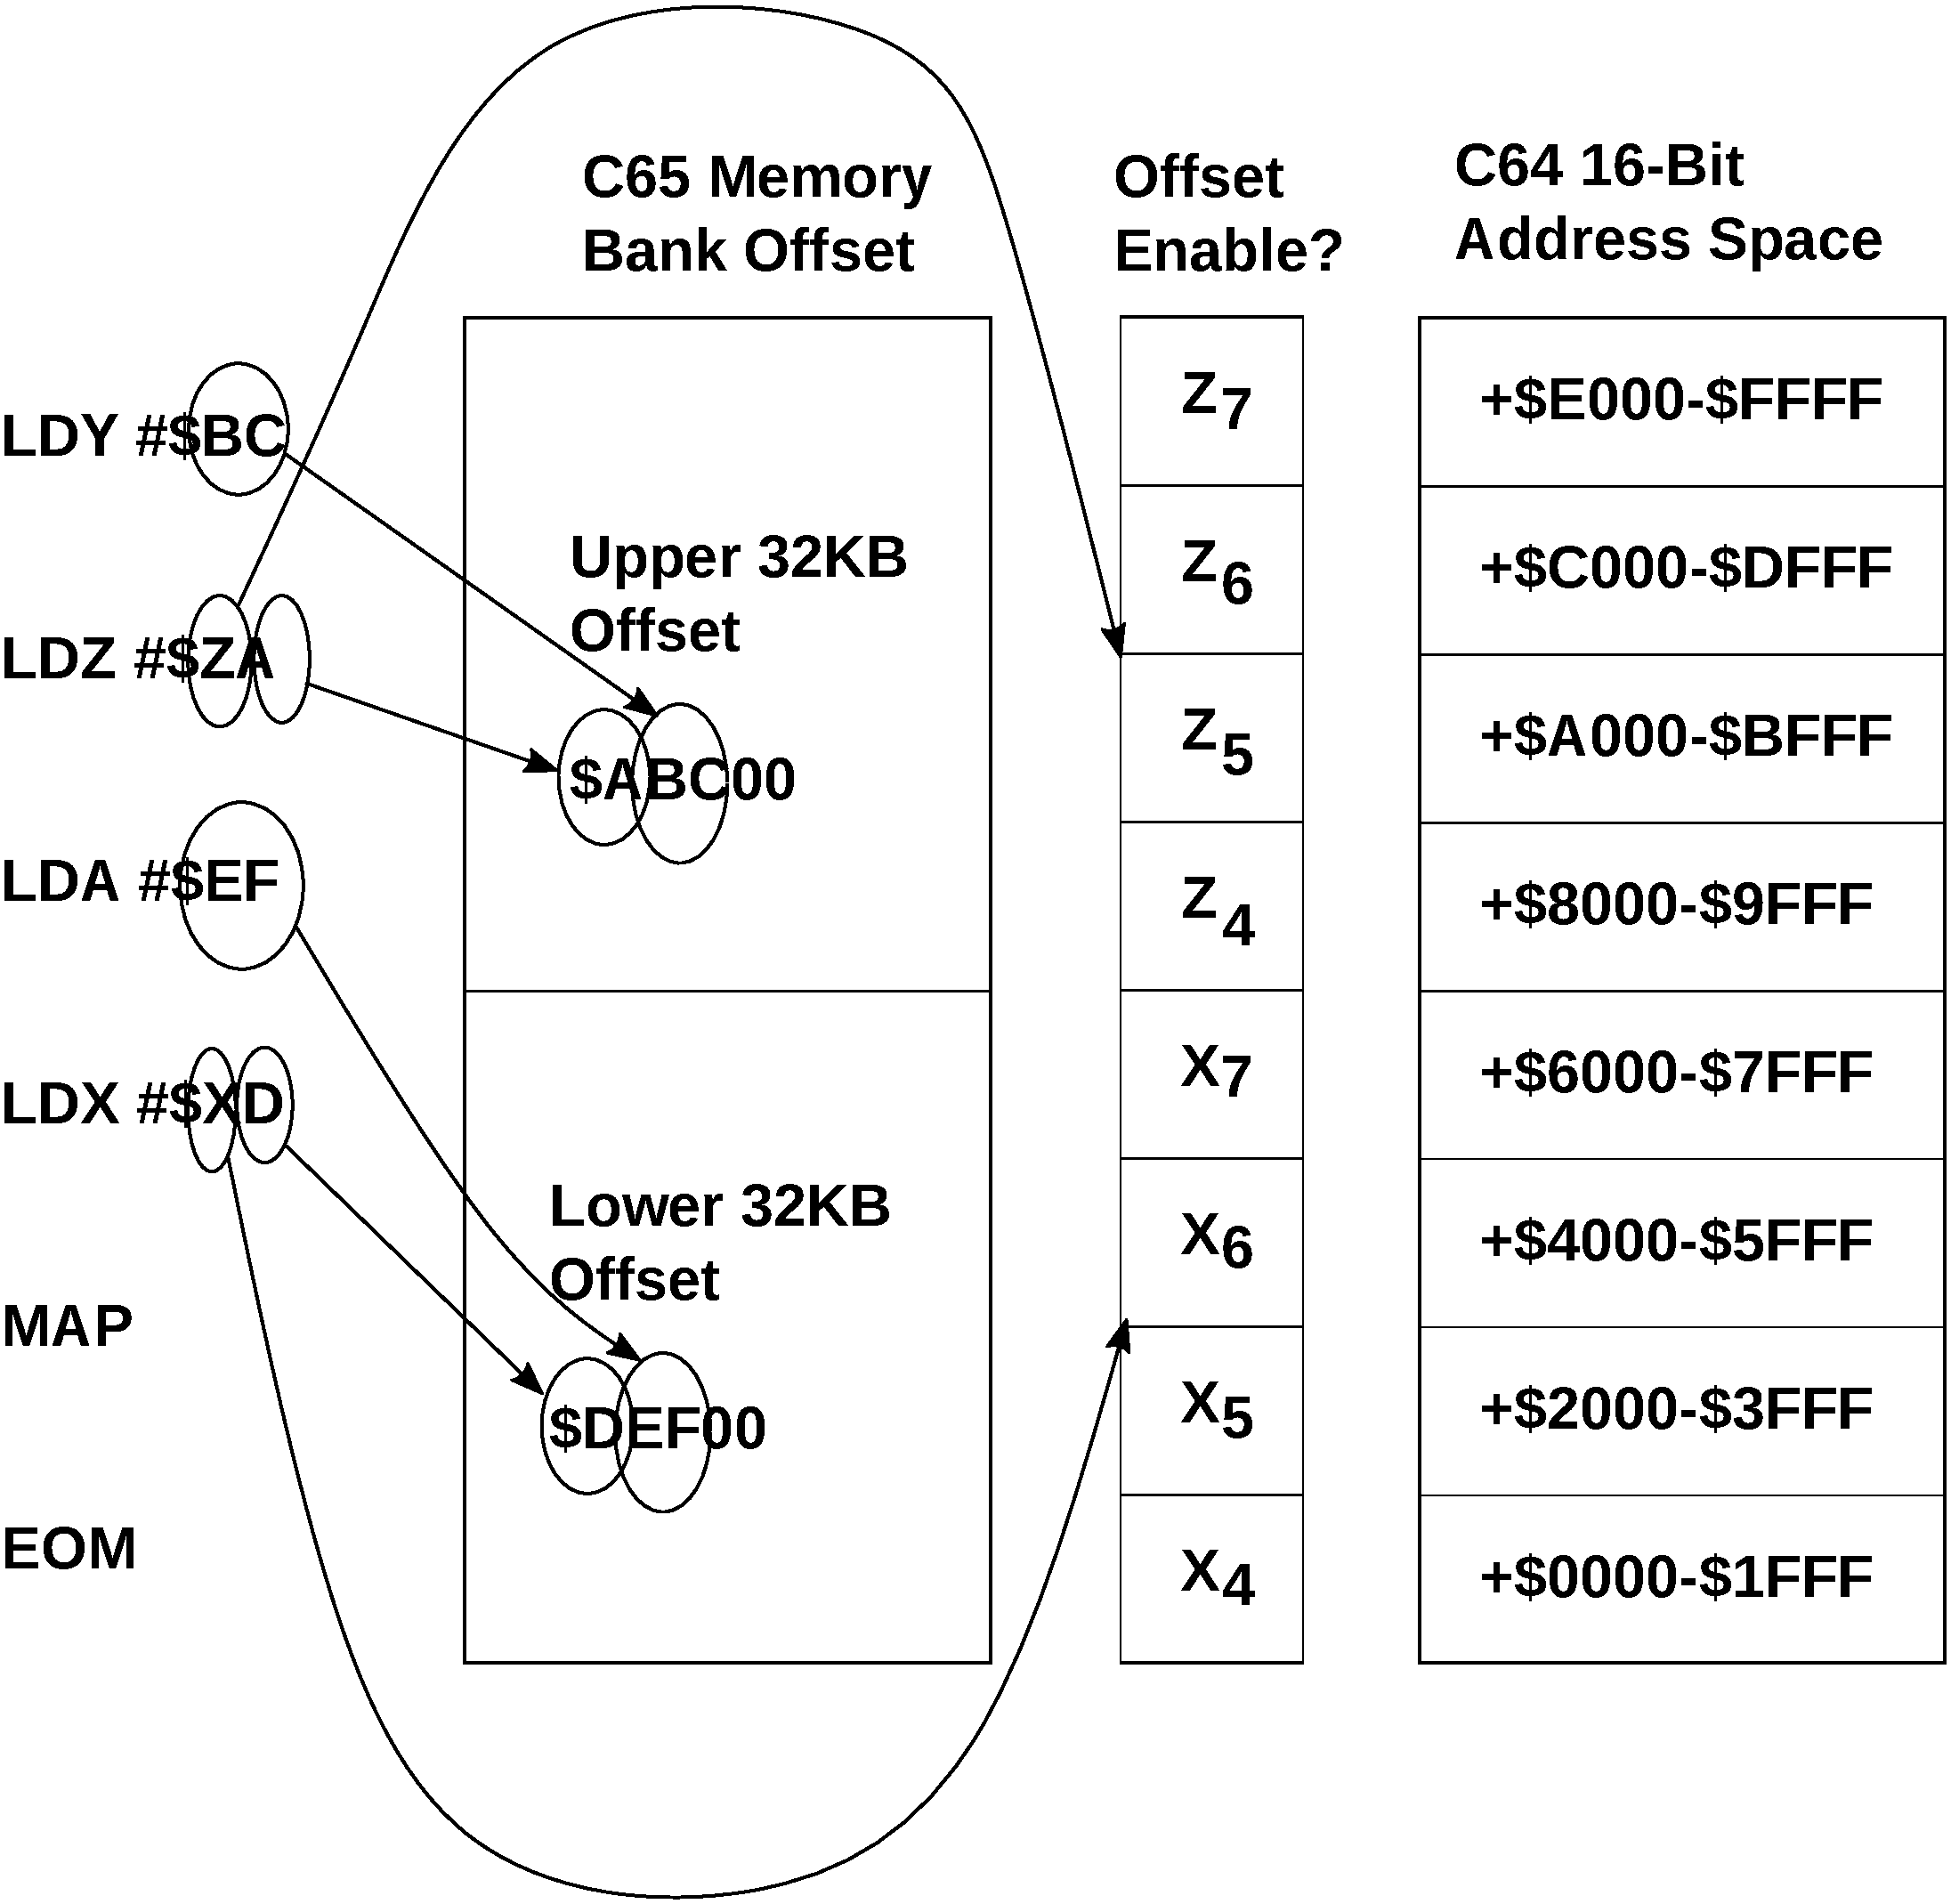
\includegraphics[width=0.75\textwidth]{images/illustrations/map-instruction-operation.pdf}\index{MAP}\index{Memory banking}
\end{center}

That is, the contents of the A register and the lower-nibble of the X register form a 12-bit value
that is multiplied by 256 to produce the offset used for any of the 8KB banks in the lower 32KB half of the 6502's 16-bit address
space.  The upper nibble of the X register is used as flags to indicate which of the four 8KB blocks in that 32KB half of the
6502 address space should have the offset added to their addresses to compute the actual address.

The Y and Z registers are used in a similar way to produce the offset for the upper 32KB half of the 6502 address space, and the
flags to indicate whether the offset is used for each of the four 8KB blocks in that half of the address space.

Note that the lower 8 bits of the offset cannot be set. That is, the offset will be a multiple of 256
bytes, unlike on some extended 6502 processors.  However, in practice this restriction is rarely
limiting.

To understand how this works in practice, the following example shows how this works with a concrete
example, showing the address ranges that would be visible in each of the 8KB slices of the 6502's
64KB address space:

\begin{center}
  \includegraphics[width=0.75\textwidth]{images/illustrations/map-instruction-operation-example1.pdf}\index{MAP}\index{Memory banking}
\end{center}

Notice that the offsets for each of the two 32KB address ranges get added to the 6502 address.
This is why the offset of \$48000 for the upper 32KB generates an address of \$50000 at the 6502
address \$8000.

See also under ``Using the MAP instruction to access >1MB'' for further explanation.

\subsubsection{Direct Memory Access (DMA) Controller}

The C65's F018/F018A DMA controller allows for rapid filling, copying and swapping of the contents of memory
anywhere in the 1MB address space. Detailed information about the F018 DMA controller, and the MEGA65's
enhancements to this, refer to \bookvref{cha:dmagic}

\subsubsection{Flat Memory Access}

\subsection{Accessing memory beyond the 1MB point}
\label{sec:extended-memory}

The MEGA65 can support up to 256MB of memory. This is more than the 1MB address space of the CSG4510
on which it is based. There are several ways of performing this.

\subsubsection{Using the MAP instruction to access >1MB}

The full address space is available to the MAP instruction for legacy C65-style memory
mapping, although some care is required, as the MAP instruction must be called up to three times.
The reason for this is that the MAP instruction must be called to first select which mega-byte of
memory will be used for the lower and upper map regions, before it is again called in the normal
way to set the memory mapping.  Because between these two calls the memory mapping offset will be
a mix of the old and new addresses, all mapping should be first disabled via the MAP instruction.
This means that the code to re-map memory should live in the bottom 64KB of RAM or in one of the
ROM-bankable regions, so that it can remain visible during the mapping process.

Failure to handle this situation properly will result in the processor executing instructions
from somewhere unexpected half-way through the process, because the routine it is executing
to perform the mapping will suddenly no longer be mapped.

Because of the relative complexity of this process, and the other problems with the MAP instruction
as a means of memory access, we recommend that for accessing data outside of the current memory
map that you use either DMA or the flat-memory address features of the 45GS02 that are described below.
Indeed, access to the full address space via the MAP instruction is only provided for completeness.

As an other example of how the MAP instruction can be used to map an area of memory from
the expanded address space, the following program maps the Ethernet frame buffer from its natural location
at \$FFDE8000 to appear at \$6800.  To keep the example as simple as possible, we assume that the code
is running from in the bottom 64KB of RAM, and not in the region between \$6000 -- \$8000.

As the MAP instruction normally is only aware of the C65-style 20-bit addresses, the MEGA65 extension to the
instruction must be used to set the upper 8 bits of the 28-bit MEGA65 addresses, i.e., which mega-byte of address
space should be used for the address translation.  This is done by setting the X
register to \$0F when setting the mega-byte number for the lower-32KB of the C64-style 64KB address space.
This does not create any incompatibility with any sensible use of the MAP instruction on a C65, because this
value indicates that none of the four 8KB memory blocks will be re-mapped, but at the same time specifies that
the upper 4 bits of the address offset for re-mapped block is the non-zero value of \$F.  The mega-byte number
is then specified by setting the A register.

The same approach applies to the upper 32KB, but using the Z and Y
registers instead of the X and A registers.  However, in this case, we do not need to re-map the upper 32KB of
memory in this example, we will leave the Z and Y registers set to zero.  We must however set X and A to
set the mega-byte number for the lower-32KB to \$FF. Therefore A must have the value \$FF.  To set the lower 20-bits
of the address offset we use the MAP instruction a second time, this time using it in the normal C65 manner.
As we want to remap \$6800 to \$FFDE800, and have already dealt with the \$FFxxxxx offset via the mega-byte number,
we need only to apply the offset to make \$6800 point to \$DE800. \$DE800 minus \$6800 = \$D8000.  As the MAP instruction
operates with a mapping granularity of 256 bytes = \$100, we can drop the last two digits from \$D8000 to obtain the
MAP offset of \$D80. The lower 8-bits, \$80, must be loaded into the A register. The upper 4-bits, \$D, must be loaded into
the low-nibble of the X register.  As we wish to apply the mapping to only the fourth of the 8KB blocks that make up the
lower 32KB half of the C64 memory map, we must set the 4th bit of the upper nibble. That is, the upper nibble must be set
to \%1000, i.e., \$8.  Therefore the X register must be loaded with \$8D.  Thus we yield the complete example program:

\begin{screenoutput}
; Map Ethernet registers at $6000 - $7FFF

; Ethernet controller really lives $FFDE000 - $FFDEFFF, so select $FF megabyte section for MAP LO
LDA #$ff
LDX #$0f
LDY #$00
LDZ #$00
map

; now enable mapping of $DE000-$DFFFF at $6000
; MAPs are offset based, so we need to subtract $6000 from the target address
; $DE000 - $6000 = $D8000
LDA #$80
LDX #$8d
LDY #$00
LDZ #$00
map
EOM

; Ethernet buffer now visible at $6800 - $6FFF
\end{screenoutput}

Note that the EOM (End Of Mapping) instruction (which is the same as NOP on a 6502, i.e., opcode \$EA) was only supplied after the last MAP instruction, to make sure that no interrupts could occur while
the memory map contained mixed values with the mega-byte number set, but the lower-bits of the mapping address had not been
updated.

No example in BASIC for the MAP instruction is possible, because the MAP is an machine code instruction of the 4510 / 45GS02 processors.

\subsubsection{Flat-Memory Access}

The 45GS02 makes it easy to read or write a byte from anywhere in memory by allowing the Zero-Page Indirect
addressing mode to use a 32-bit pointer instead of the normal 16-bit pointer.  This is accomplished by
using the Z-indexed Zero-Page Indirect Addressing Mode for the access, and having the instruction directly
preceded by a NOP instruction (opcode \$EA).  For example:

\begin{screenoutput}
NOP
LDA ($45),Z
\end{screenoutput}

If you are using the ACME assembler, or another assembler that supports the 45GS02 extensions, you can instead use square-brackets
to indicate that you are performing a flat-memory operation. Such assemblers will insert the \$EA prefix automatically for you. For example:

\begin{screenoutput}
LDA [$45],Z
\end{screenoutput}

Regardless which tool you are using, this example would read the four bytes of Zero-Page memory at \$45 -- \$48 to form a 32-bit memory address, and add the value of the
Z register to this to form the actual address that will be read from.  The byte order in the address is the same as
the 6502, i.e., the right-most (least significant) byte of the address will be read from the first address (\$45 in this case),
and so on, until the left-most (most significant) byte will be read from \$48.  For example, to read from memory location
\$12345678, the contents of memory beginning at \$45 should be 78 56 34 12.

This method is much more efficient and also simpler than either using the MAP instruction or the DMA controller for single memory accesses,
and is what we generally recommend.  The DMA controller can be used for moving/filler larger regions of memory.
We recommend the MAP instruction only be used for banking code, or in rare situations where extensive access to a small region of
memory is required, and the extra cycles of reading the 32-bit addresses is problematic.

\subsection{Virtual 32-bit Register}

The 45GS02 allows the use of its four general purpose registers, A, X, Y and Z (A is LSB, Z is MSB) as a single virtual 32-bit register, 
also called the {\em Q pseudo register}.
This can greatly simplify and speed up many common operations, and help avoid many common programming errors.
For example, adding two 16-bit or 32-bit values can now be easily accomplished with something like:

\begin{screenoutput}
  ; Clear carry before performing addition, as normal
  CLC
  ; Prefix an instruction with two NEG instructions to select virtual 32-bit register mode
  NEG
  NEG
  LDA $1234  ; Load the contents of $1234-$1237 into A,X,Y and Z respectively
  ; And again, for the addition
  NEG
  NEG
  ADC $1238  ; Add the contents of $1238-$123B
  ; The result of the addition is now in A, X, Y and Z.
  ; And can be written out in whole or part

  ; To write it all out, again, we need the NEG + NEG prefix
  NEG
  NEG
  STA $123C ; Write the whole out to $123C-$123F

  ; Or to write out the bottom bytes, we can just write the contents of A and X as normal
  STA $1240
  STX $1241
\end{screenoutput}

This approach works with the LDA, STA, ADC, SBC, CMP, EOR, AND, BIT, ORA, ASL, ASR, LSR, ROL, ROR, INC and DEC instructions.
If you are using ACME or another 45GS02 aware assembler, you can instead use the new \stw{LDQ}, \stw{STQ}, \stw{ADCQ},
\stw{SBCQ}, \stw{CPQ}, \stw{EORQ}, \stw{ANDQ}, \stw{BITQ}, \stw{ORQ}, \stw{ASLQ}, \stw{ASRQ}, \stw{LSRQ}, \stw{ROLQ}, \stw{RORQ}, \stw{INQ} and \stw{DEQ}
mnemonics.\index{LDQ}\index{STQ}\index{ADCQ}\index{SBCQ}\index{CPQ}\index{EORQ}\index{ANDQ}\index{BITQ}\index{ORQ}\index{ASLQ}\index{ASRQ}\index{LSRQ}\index{ROLQ}\index{RORQ}\index{INQ}\index{DEQ} The previous example would thus become:

\begin{screenoutput}
  ; Clear carry before performing addition, as normal
  CLC
  LDQ  $1234  ; Load the contents of $1234-$1237 into A,X,Y and Z respectively
  ADCQ $1238  ; Add the contents of $1238-$123B
  ; The result of the addition is now in A, X, Y and Z.
  ; And can be written out in whole or part

  ; To write it all out, again, we need the NEG + NEG prefix
  STQ $123C ; Write the whole out to $123C-$123F

  ; Or to write out the bottom bytes, we can just write the contents of A and X as normal
  STA $1240
  STX $1241
\end{screenoutput}

The virtual 32-bit addressing mode works with any addressing mode.
However, indexed addressing modes, where X, Y or Z are added to the address should
be used with care, because these registers may in fact be holding part of a 32-bit value.

The exception is the Zero-Page Indirect Z-Indexed addressing mode: In this case the Z register is NOT added to the target address
(with the exception of the LDQ opcode), unlike would normally be the case. This is to allow the virtual 32-bit register to be able
to be used with flat-memory access with the combined prefix of \stw{NEG NEG NOP},  before the instruction to allow accessing a
32-bit value anywhere in memory in a single instruction.

Note that the virtual 32-bit register cannot be used in immediate mode, e.g., to load a constant into the four general
purpose registers, or to add or subtract a constant value.  This is to avoid problems with variable length instructions.

For LDQ and STQ, it would save at most one byte
compared to LDA \#\$nn ... LDZ \#\$nn, and would be no faster.  In fact, for many common
values, such as \#\$00000000, there are short-cuts, such as:

\begin{screenoutput}
LDA #$00
TAX
TAY
TAZ
\end{screenoutput}

If you need to add or subtract a 32-bit immediate value, this may require you to re-order the arguments, or perform other
minor gymnastics.  For example, to compute the sum of the contents of memory and an immediate value, you can load the A, X, Y
and Z registers with the immediate value, and then use \stw{ADCQ} with the memory address, e.g.:

\begin{screenoutput}
  ; Get the immediate value #$12345678 into Q
  LDA #$78
  LDX #$56
  LDY #$34
  LDZ #$12
  ; Add the contents of memory locations $1234-$1237
  NEG
  NEG
  ADC $1234
  ; Store the result back in $1234-$1237
  NEG
  NEG
  STA $1234
\end{screenoutput}

Again, if you are using the ACME or another 45GS02-aware assembler, this can be more compactly and
clearly written as follows. But note that in both cases the same byte-sequence of machine code is
produced, and the program will take the same number of cycles to execute.

\begin{screenoutput}
  ; Get the immediate value #$12345678 into Q
  LDA #$78
  LDX #$56
  LDY #$34
  LDZ #$12
  ; Add the contents of memory locations $1234-$1237
  ADCQ $1234
  ; Store the result back in $1234-$1237
  STQ $1234
\end{screenoutput}

\section{C64 CPU Memory Mapped Registers}

\input{regtable_CPU.C64}

\section{New CPU Memory Mapped Registers}

\input{regtable_CPU.MEGA65}

\section{MEGA65 CPU Maths Acceleration Registers}

Every MEGA65 contains a combined 32-bit hardware multiplier and divider.
This device takes two 32-bit inputs, {\bf MULTINA} and {\bf MULTINB}, and simultaneously calculates:

\begin{itemize}
\item the 64-bit product {\bf MULTOUT} of {\bf MULTINA} and {\bf MULTINB}
\item the 32-bit whole part {\bf DIVOUT}(4-7) of {\bf MULTINA} divided by {\bf MULTINB}
\item the 32-bit fractional part {\bf DIVOUT}(0-3) of {\bf MULTINA} divided by {\bf MULTINB}
\end{itemize}

It is always updating the outputs based on the inputs, so there is no need to take special action when changing the inputs.
The multiplier takes 1 cycle to calculate, and the updated result will thus be available immediately (a {\bf MULBUSY} bit is
defined, but currently it won't be set at all). The hardware divider, however, can take upto 20 cycles depending on the
particular inputs. The programmer should check the {\bf DIVBUSY} bit if the divider is still calculating:

\begin{screenoutput}
loop:   BIT $D70F   ; transfer DIVBUSY bit into N flag
        BMI loop    ; as long as it is set, we need to wait
\end{screenoutput}

The MEGA65 is planned to also include a programmable math unit, which helps to accelerate the calculation of fixed-point formulae.
This is presently disabled and will be further documented if and when it becomes available (addresses \$D780 - \$D7E3).

\input{regtable_MATH.MEGA65}

\section{MEGA65 Hypervisor Mode}
\label{sec:hypervisor-mode}

\subsection{Reset}

On power-up or reset, the MEGA65 starts up in hypervisor mode, and expects to find a program in the
16KB hypervisor memory, and begins executing instructions at address \$8100.  Normally a JMP instruction
will be located at this address, that will jump into a reset routine. That is, the 45GS02
does not use the normal 6502 reset vector. It's function is emulated by the Hyppo hypervisor program,
which fetches the address from the 6502 reset vector in the loaded client operating system when
exiting hypervisor mode.

The hypervisor memory is automatically mapped on reset to \$8000 - \$BFFF.  This special memory is not
able to mapped or in anyway accessed, except when in hypervisor mode. It can, however, always be accessed from the serial monitor/debugger
interface via its 28-bit address, \$FFF8000 -- \$FFFBFFF.  This is to protect it from accidental or malicious access from a guest operating system.

\subsection{Entering / Exiting Hypervisor Mode}

Entering the Hypervisor occurs whenever any of the following events occurs:

\begin{itemize}
\item{\bf Power-on} When the MEGA65 is first powered on.
\item{\bf Reset} If the reset line is lowered, or a watch-dog triggered reset occurs.
\item{\bf SYSCALL register accessed} The registers \$D640 - \$D67F in the MEGA65 I/O context trigger SYSCALLs when accessed.
  This is intended to be the mechanism by which a client operating system or process requests the attention of the hypervisor or operating system.
\item{\bf Page Fault} On MEGA65s that feature virtual memory, a page fault will cause a trap to hypervisor mode.
\item{\bf Certain keyboard events} Pressing \widekey{RESTORE} for >0.5 seconds, or the \specialkey{ALT} and
\specialkey{TAB} key combination traps to the hypervisor.  Typically the first is used to launch the Freeze Menu an the second to toggle the display of debug interface.
\item{\bf Accessing virtualised I/O devices} For example, if the F011 (internal 3.5'' disk drive controller) has been virtualised, then attempting to read or write sectors using this device will cause traps to the hypervisor.
  \item{\bf Executing an instruction that would lock up the CPU} A number of undocumented opcodes on the 6502 will cause the CPU to lockup.  On the MEGA65, instead of locking up, the computer will trap to the hypervisor.  This could be used to implement alternative instruction behaviours, or simply to tell the user that something bad has happened.
  \item{\bf Certain special events} Some devices can generate hypervisor-level interrupts. These are implemented as traps to the hypervisor.
\end{itemize}

The 45GS02 handles all of these in a similar manner internally:

\begin{enumerate}
\item The SYSCALL or trap address is calculated, based on the event.
\item The contents of all CPU registers are saved into the virtualisation control registers.
\item The hypervisor mode memory layout is activated, the CPU decimal flag and special purpose registers are all set to appropriate values.  The contents of the A,X,Y and Z and most other CPU flags are preserved, so that they can be accessed from the Hypervisor's SYSCALL/trap handler routine, without having to load them, thus saving a few cycles for each call.
\item The hypervisor-mode flag is asserted, and the program counter (PC) register is set to the computed address.
\end{enumerate}

All of the above happens in one CPU cycle, i.e., in 25 nano-seconds.
Returning from a SYSCALL or trap consists simply of writing to \$D67F, which
requires 125 nano-seconds, for a total overhead of 150 nano-seconds.
This gives the MEGA65 SYSCALL performance rivalling -- even beating
-- even the fastest modern computers, where the system call latency is
typically hundreds to tens of thousands of cycles \cite{soares2010flexsc}.

\subsection{Hypervisor Memory Layout}

The hypervisor memory is 16KB in size.  The first 512 bytes are
reserved for SYSCALL and system trap entry
points, with four bytes for each.  For example, the reset entry point is
at \$8100 - \$8100 + 3 = \$8100 - \$8103.
This allows 4 bytes for an instruction, typically a JMP instruction,
followed by a NOP to pad it to 4 bytes.

The full list of SYSCALLs and traps is:

\begin{longtable}{|L{1.2cm}|L{1.1cm}|C{2cm}|L{6cm}|}
\hline
{\bf{HEX}} & {\bf{DEC}} & {\bf{Name}} & {\bf{Description}} \\
\hline
\endfirsthead
\multicolumn{3}{l@{}}{\ldots continued}\\
\hline
{\bf{HEX}} & {\bf{DEC}} & {\bf{Name}} & {\bf{Description}} \\
\hline
\endhead
\multicolumn{3}{l@{}}{continued \ldots}\\
\endfoot
\hline
\endlastfoot
\small  8000 & \small 32768 & SYSCALL00 & SYSCALL 0 entry point \\
\hline
\small  8004 & \small 32772 & SYSCALL01 & SYSCALL 1 entry point \\
\hline
\small  8008 & \small 32776 & SYSCALL02 & SYSCALL 2 entry point \\
\hline
\small  800C & \small 32780 & SYSCALL03 & SYSCALL 3 entry point \\
\hline
\small  8010 & \small 32784 & SYSCALL04 & SYSCALL 4 entry point \\
\hline
\small  8014 & \small 32788 & SYSCALL05 & SYSCALL 5 entry point \\
\hline
\small  8018 & \small 32792 & SYSCALL06 & SYSCALL 6 entry point \\
\hline
\small  801C & \small 32796 & SYSCALL07 & SYSCALL 7 entry point \\
\hline
\small  8020 & \small 32800 & SYSCALL08 & SYSCALL 8 entry point \\
\hline
\small  8024 & \small 32804 & SYSCALL09 & SYSCALL 9 entry point \\
\hline
\small  8028 & \small 32808 & SYSCALL0A & SYSCALL 10 entry point \\
\hline
\small  802C & \small 32812 & SYSCALL0B & SYSCALL 11 entry point \\
\hline
\small  8030 & \small 32816 & SYSCALL0C & SYSCALL 12 entry point \\
\hline
\small  8034 & \small 32820 & SYSCALL0D & SYSCALL 13 entry point \\
\hline
\small  8038 & \small 32824 & SYSCALL0E & SYSCALL 14 entry point \\
\hline
\small  803C & \small 32828 & SYSCALL0F & SYSCALL 15 entry point \\
\hline
\small  8040 & \small 32832 & SYSCALL10 & SYSCALL 16 entry point \\
\hline
\small  8044 & \small 32836 & SECURENTR & Enter secure container trap entry point \\
\hline
\small  8048 & \small 32840 & SECUREXIT & Leave secure container trap entry point. \\
\hline
\small  804C & \small 32844 & SYSCALL13 & SYSCALL 19 entry point \\
\hline
\small  8050 & \small 32848 & SYSCALL14 & SYSCALL 20 entry point \\
\hline
\small  8054 & \small 32852 & SYSCALL15 & SYSCALL 21 entry point \\
\hline
\small  8058 & \small 32856 & SYSCALL16 & SYSCALL 22 entry point \\
\hline
\small  805C & \small 32860 & SYSCALL17 & SYSCALL 23 entry point \\
\hline
\small  8060 & \small 32864 & SYSCALL18 & SYSCALL 24 entry point \\
\hline
\small  8064 & \small 32868 & SYSCALL19 & SYSCALL 25 entry point \\
\hline
\small  8068 & \small 32872 & SYSCALL1A & SYSCALL 26 entry point \\
\hline
\small  806C & \small 32876 & SYSCALL1B & SYSCALL 27 entry point \\
\hline
\small  8070 & \small 32880 & SYSCALL1C & SYSCALL 28 entry point \\
\hline
\small  8074 & \small 32884 & SYSCALL1D & SYSCALL 29 entry point \\
\hline
\small  8078 & \small 32888 & SYSCALL1E & SYSCALL 30 entry point \\
\hline
\small  807C & \small 32892 & SYSCALL1F & SYSCALL 31 entry point \\
\hline
\small  8080 & \small 32896 & SYSCALL20 & SYSCALL 32 entry point \\
\hline
\small  8084 & \small 32900 & SYSCALL21 & SYSCALL 33 entry point \\
\hline
\small  8088 & \small 32904 & SYSCALL22 & SYSCALL 34 entry point \\
\hline
\small  808C & \small 32908 & SYSCALL23 & SYSCALL 35 entry point \\
\hline
\small  8090 & \small 32912 & SYSCALL24 & SYSCALL 36 entry point \\
\hline
\small  8094 & \small 32916 & SYSCALL25 & SYSCALL 37 entry point \\
\hline
\small  8098 & \small 32920 & SYSCALL26 & SYSCALL 38 entry point \\
\hline
\small  809C & \small 32924 & SYSCALL27 & SYSCALL 39 entry point \\
\hline
\small  80A0 & \small 32928 & SYSCALL28 & SYSCALL 40 entry point \\
\hline
\small  80A4 & \small 32932 & SYSCALL29 & SYSCALL 41 entry point \\
\hline
\small  80A8 & \small 32936 & SYSCALL2A & SYSCALL 42 entry point \\
\hline
\small  80AC & \small 32940 & SYSCALL2B & SYSCALL 43 entry point \\
\hline
\small  80B0 & \small 32944 & SYSCALL2C & SYSCALL 44 entry point \\
\hline
\small  80B4 & \small 32948 & SYSCALL2D & SYSCALL 45 entry point \\
\hline
\small  80B8 & \small 32952 & SYSCALL2E & SYSCALL 46 entry point \\
\hline
\small  80BC & \small 32956 & SYSCALL2F & SYSCALL 47 entry point \\
\hline
\small  80C0 & \small 32960 & SYSCALL30 & SYSCALL 48 entry point \\
\hline
\small  80C4 & \small 32964 & SYSCALL31 & SYSCALL 49 entry point \\
\hline
\small  80C8 & \small 32968 & SYSCALL32 & SYSCALL 50 entry point \\
\hline
\small  80CC & \small 32972 & SYSCALL33 & SYSCALL 51 entry point \\
\hline
\small  80D0 & \small 32976 & SYSCALL34 & SYSCALL 52 entry point \\
\hline
\small  80D4 & \small 32980 & SYSCALL35 & SYSCALL 53 entry point \\
\hline
\small  80D8 & \small 32984 & SYSCALL36 & SYSCALL 54 entry point \\
\hline
\small  80DC & \small 32988 & SYSCALL37 & SYSCALL 55 entry point \\
\hline
\small  80E0 & \small 32992 & SYSCALL38 & SYSCALL 56 entry point \\
\hline
\small  80E4 & \small 32996 & SYSCALL39 & SYSCALL 57 entry point \\
\hline
\small  80E8 & \small 33000 & SYSCALL3A & SYSCALL 58 entry point \\
\hline
\small  80EC & \small 33004 & SYSCALL3B & SYSCALL 59 entry point \\
\hline
\small  80F0 & \small 33008 & SYSCALL3C & SYSCALL 60 entry point \\
\hline
\small  80F4 & \small 33012 & SYSCALL3D & SYSCALL 61 entry point \\
\hline
\small  80F8 & \small 33016 & SYSCALL3E & SYSCALL 62 entry point \\
\hline
\small  80FC & \small 33020 & SYSCALL3F & SYSCALL 63 entry point \\
\hline
\small  8100 & \small 33024 & RESET & Power-on/reset entry point \\
\hline
\small  8104 & \small 33028 & PAGFAULT & Page fault entry point (not currently used) \\
\hline
\small  8108 & \small 33032 & RESTORKEY & Restore-key long press trap entry point \\
\hline
\small  810C & \small 33036 & ALTTABKEY & ALT+TAB trap entry point \\
\hline
\small  8110 & \small 33040 & VF011RD & F011 virtualised disk read trap entry point \\
\hline
\small  8114 & \small 33044 & VF011WR & F011 virtualised disk write trap entry point \\
\hline
\small  8118 & \small 33048 & BREAKPT & CPU break-point encountered \\
\hline
\small  811C -- 81FB & \small 33048 -- 33275 & RESERVED & Reserved traps point entry \\
\hline
\small  81FC & \small 33276 & CPUKIL & KIL instruction in 6502-mode trap entry point \\
\hline
\end{longtable}

The remainder of the 16KB hypervisor memory is available for use by the programmer, but
will typically use the last 512 bytes for the stack and zero-page, giving an overall memory map as follows:

\begin{longtable}{|L{1.2cm}|L{1.1cm}|L{8cm}|}
\hline
{\bf{HEX}} & {\bf{DEC}} & {\bf{Description}} \\
\hline
\endfirsthead
\multicolumn{3}{l@{}}{\ldots continued}\\
\hline
{\bf{HEX}} & {\bf{DEC}} & {\bf{Description}} \\
\hline
\endhead
\multicolumn{3}{l@{}}{continued \ldots}\\
\endfoot
\hline
\endlastfoot
\small  8000 -- 81FF & \small 32768 -- 33279 & SYSCALL and trap entry points \\
\hline
\small  8200 -- BDFF & \small 33280 -- 48639 & Available for hypervisor or operating system program \\
\hline
\small  8E00 -- BEFF & \small 48640 -- 48895 & Processor stack for hypervisor or operating system \\
\hline
\small  8F00 -- BFFF & \small 48896 -- 49151 & Processor zero-page storage for hypervisor or operating system \\
\hline
\end{longtable}

The stack is used for holding the return address of function calls.  The zero-page storage is typically used for holding
variables and other short-term storage, as is customary on the 6502.

\subsection{Hypervisor Virtualisation Control Registers}

\input{regtable_HCPU.MEGA65}

\subsection{Programming for Hypervisor Mode}

The easiest way to write a program for Hypervisor Mode on the MEGA65 is to use KickC, which is a special version of C
made for writing programs for 6502-class processors.  The following example programs are from KickC's supplied examples.
KickC produces very efficient code, and directly supports the MEGA65's
hypervisor mode quite easily through the use of a linker definition file with the following contents:

\begin{screenoutput}
.file [name="%O.bin", type="bin", segments="XMega65Bin"]
.segmentdef XMega65Bin [segments="Syscall, Code, Data, Stack, Zeropage"]
.segmentdef Syscall [start=$8000, max=$81ff]
.segmentdef Code [start=$8200, min=$8200, max=$bdff]
.segmentdef Data [startAfter="Code", min=$8200, max=$bdff]
.segmentdef Stack [min=$be00, max=$beff, fill]
.segmentdef Zeropage [min=$bf00, max=$bfff, fill]
\end{screenoutput}

This file instructs KickC's assembler to create a 16KB file with the 512 byte SYSCALL/trap entry point region at the start,
followed by code and data areas, and then the stack and zero-page areas. It enforces the size and location of these fields, and
will give an error during compilation if anything is too big to fit.

With this file in place, you can then create a KickC source file that provides data structures for the SYSCALL/trap table, e.g.:

\begin{screenoutput}
// XMega65 KERNAL Development Template
// Each function of the KERNAL is a no-args function
// The functions are placed in the SYSCALLS table surrounded by JMP and NOP

import "string"

// Use a linker definition file (put the previous listing into that file)
#pragma link("mega65hyper.ld")

// Some definitions of addresses and special values that this program uses
const char* RASTER = 0xd012;
const char* VIC_MEMORY = 0xd018;
const char* SCREEN = 0x0400;
const char* BGCOL = 0xd021;
const char* COLS = 0xd800;
const char BLACK = 0;
const char WHITE = 1;

// Some text to display
char[] MESSAGE = "hello world!";
\end{screenoutput}

\begin{screenoutput}
void main() {
    // Initialise screen memory, and select correct font
    *VIC_MEMORY = 0x14;
    // Fill the screen with spaces
    memset(SCREEN, ' ', 40*25);
    // Set the colour of every character on the screen to white
    memset(COLS, WHITE, 40*25);
    // Print the "hello world!" message
    char* sc = SCREEN+40;  // Display it one line down on the screen
    char* msg = MESSAGE; // The massage to display
    // A simple copy routine to copy the string
    while(*msg) {
        *sc++ = *msg++;
    }
    // Loop forever showing two white lines as raster bars
    while(true) {
        if(*RASTER==54 || *RASTER==66) {
            *BGCOL = WHITE;
        } else {
            *BGCOL = BLACK;
        }
    }
}

// Here are a couple sample SYSCALL handlers that just display a character on the screen
void syscall1() {
    *(SCREEN+79) = '>';
}

void syscall2() {
    *(SCREEN+78) = '<';
}

// Now we select the SYSCALL segment to hold the SYSCALL/trap entry point table.
#pragma data_seg(Syscall)

// The structure of each entry point is JMP <handler address> + NOP.
// We have a char (xjmp) to hold the opcode for the JMP instruction,
// and then put the address of the SYSCALL/trap handler in the next
// two points as a pointer, and end with the NOP instruction opcode.
\end{screenoutput}

\begin{screenoutput}
struct SysCall {
    char xjmp;         // Holds $4C, the JMP $nnnn opcode
    void()* syscall;   // Holds handler address, will be the target of the JMP
    char xnop;         // Holds $EA, the NOP opcode
};

// To save writing 0x4C and 0xEA all the time, we define them as constants
const char JMP = 0x4c;
const char NOP = 0xea;

// Now we can have a nice table of up to 64 SYSCALL handlers expressed
// in a fairly readable and easy format.
// Each line is an instance of the struct SysCall from above, with the JMP
// opcode value, the address of the handler routine and the NOP opcode value.
export struct SysCall[] SYSCALLS = {
    { JMP, &syscall1, NOP },
    { JMP, &syscall2, NOP }
    };

// In this example we had only two SYSCALLs defined, so rather than having
// another 62 lines, we can just ask KickC to make the TRAP table begin
// at the next multiple of $100, i.e., at $8100.
export align(0x100) struct SysCall[] SYSCALL\_RESET = {
    { JMP, &main, NOP }
};
\end{screenoutput}

If you save the first listing into a file called mega65hyper.ld, and the second
into a file called mega65hyper.kc, you can then compile them using KickC with
a command like:

\begin{screenoutput}
  kickc -a mega65hyper
\end{screenoutput}

It will then produce a file called mega65hyper.bin, which you can then try out
on your MEGA65, or run in the XMega65 emulator with a command like:

\begin{screenoutput}
  xmega65 -kickup mega65hyper.bin
\end{screenoutput}

  \chapter{VIC-IV Video Interface Controller}
\label{cha:viciv}

\section{Features}
The VIC-IV is a fourth generation Video Interface Controller developed
especially for the MEGA65, and featuring very good backwards compatibility
with the VIC-II that was used in the C64, and the VIC-III that
was used in the C65.  The VIC-IV can be programmed as though it were either
of those predecessor systems.  In addition it supports a number of new
features. It is easy to mix older VIC-II/III features with the new VIC-IV
features, making it easy to transition from the VIC-II or VIC-III to the VIC-IV,
just as the VIC-III made it easy to transition from the VIC-II.  Some of the new
features and enhancements of the VIC-IV include:

\begin{itemize}
\item {\bf Direct access to 384KB RAM} (up from 16KB/64KB with the VIC-II and 128KB
  with the VIC-III).
\item Support for {\bf 32KB of 8-bit Colour/Attribute RAM} (up from 2KB on the VIC-III), to
  support very large screens.
\item {\bf HDTV 720$\times$576 / 800$\times$600 native resolution} at both 50Hz and 60Hz for {\bf PAL and NTSC}, with {\bf VGA and digital video} output.
\item {\bf 81MHz pixel clock} (up from $\sim$ 8MHz with the VIC-II/III), which enables a wide range of new features.
\item New 16-colour (16$\times$8 pixels per character cell) and 256-colour (8$\times$8 pixels per character cell) {\bf full-colour text modes}.
\item Support for up to {\bf 8,192 unique characters in a character set}.
\item {\bf Four 256-colour palette banks} (versus the VIC-III's single palette bank), each supporting {\bf 23-bit colour depth} (versus the VIC-III's 12-bit colour depth), and which can be rapidly alternated to create even more colourful graphics than is possible with the VIC-III.
\item Screen, bitmap, colour and character data can be positioned at any {\bf address with byte-level granularity} (compared with fixed 1KB -- 16KB boundaries with the VIC-II/III)
\item {\bf Virtual screen dimensioning}, which combined with byte-level data position granularity provides effective {\bf hardware support for scrolling and panning in both X and Y directions}.
\item {\bf New sprite modes}: Bitplane modification, {\bf full-colour} (15 foreground colours + transparency) and tiled modes, allowing a wide variety of new and exciting sprite-based effects
  \item The ability to stack sprites in a bit-planar manner to produce {\bf sprites with up to 256 colours}.
\item Sprites can use 64 bits of data per raster line, allowing {\bf sprites to be 64 pixels wide} when using VIC-II/III mono/multi-colour mode, or 16 pixels wide when using the new VIC-IV full-colour sprite mode.
\item {\bf Sprite tile mode}, which allows a sprite to be repeated horizontally across an entire raster line, allowing sprites to be used to create  animated backgrounds in a memory-efficient manner.
  \item Sprites can be configured to use a {\bf separate 256-colour palette} to that used to draw other text and graphics, allowing for a more colourful display.
  \item {\bf Super-extended attribute mode} which uses two screen RAM bytes and two colour RAM bytes per character mode, which supports a wide variety of new features including {\bf alpha-blending/anti-aliasing}, {\bf hardware kerning/variable-width characters}, hardware horizontal/vertical flipping, alternate palette selection and other powerful features that make it easy to create highly dynamic and colourful displays.
  \item {\bf Raster-Rewrite Buffer} which allows {\bf hardware-generated pseudo-sprites}, similar to ``bobs'' on Amiga\texttrademark{} computers, but with the advantage that they are rendered in the display pipeline, and thus do not need to be un-drawn and redrawn to animate them.
    \item {\bf Multiple 8-bit colour play-fields} are also possible using the Raster-Rewrite Buffer.

      In short, the VIC-IV is a powerful evolution of the VIC-II/III, while retaining the character and distinctiveness of the VIC-series of
      video controllers.

      For a full description of the additional registers that the VIC-IV provides, as well as documentation of the legacy VIC-II and VIC-III registers, refer to the corresponding sections of this appendix. The remainder of the appendix will focus on describing the capabilities and use of many of the VIC-IV's new features.
\end{itemize}

\section{VIC-II/III/IV Register Access Control}
Because the new features of the VIC-IV are all extensions to the existing VIC-II/III designs, there is no concept of having to select the mode in which the VIC-IV will operate: It is always in VIC-IV mode. However, for backwards compatibility with software, the many additional registers of the VIC-IV can be hidden, so that it appears to be either a VIC-II or VIC-III. This is done in the same manner that the VIC-III uses to hide its new features from legacy VIC-II software.

 The mechanism is the VIC-III write-only KEY register (\$D02F, 53295 decimal).  The VIC-III by default conceals its new features until a ``knock'' sequence is performed.  This consists of writing two special values one after the other to \$D02F.  The following table summarises the knock sequences supported by the VIC-IV, and indicates which are VIC-IV specific, and which are supported by the VIC-III:

\setlength{\tabcolsep}{3pt}
\begin{longtable}{|L{2.4cm}|L{2.4cm}|L{3.5cm}|L{2cm}|}
\hline
{\bf{First Value Hex (Decimal)}} & {\bf{Second Value Hex (Decimal)}} & {\bf{Effect}} & {\bf{VIC-IV Specific? }} \\
\hline
\endfirsthead
\multicolumn{3}{l@{}}{\ldots continued}\\
\hline
{\bf{First Value Hex (Decimal)}} & {\bf{Second Value Hex (Decimal)}} & {\bf{Effect}} & {\bf{VIC-IV Specific? }} \\
\hline
\endhead
\multicolumn{3}{l@{}}{continued \ldots}\\
 \endfoot
 \hline
\endlastfoot
\small \$00 (0) & \small \$00 (0) & Only VIC-II registers visible (all VIC-III and VIC-IV new registers are hidden) & No \\
 \hline
\small \$A5 (165) & \small \$96 (150) & VIC-III new registers visible & No \\
 \hline
\small \$47 (71) & \small \$53 (83) & Both VIC-III and VIC-IV new registers visible & Yes \\
 \hline
\small \$45 (69)  & \small \$54 (84) & No VIC-II/III/IV registers visible. 45E100 Ethernet controller buffers are visible instead & Yes \\
 \hline
   \end{longtable}


 \subsection{Detecting VIC-II/III/IV}

 Detecting which generation of the VIC-II/III/IV a machine is fitted with can be important for programs that support only particular generations, or that wish to vary their graphical display based on the capabilities of the machine.  While there are many possibilities for this, the following is a simple and effective method.  It relies on the fact that the VIC-III and VIC-IV do not repeat the VIC-II registers throughout the I/O address space.  Thus while \$D000 and \$D100 are synonymous when a VIC-II is present (or a VIC-III/IV is hiding their additional registers), this is not the case when a VIC-III or VIC-IV is making all of its registers visible.  Therefore presence of a VIC-III/IV can be determined by testing whether these two locations are aliases for the same register, or represent separate registers.
 The detection sequence consists of using the KEY register to attempt to make either VIC-IV or VIC-III additional registers visible. If either succeeds, then we can assume that the corresponding generation of VIC is installed. As the VIC-IV supports the VIC-III KEY knocks, we must first test for the presence of a VIC-IV.  Also, we assume that the MEGA65 starts in VIC-IV mode, even when running C65 BASIC.  Thus the test can be done in BASIC from either C64 or C65-mode as follows:

\begin{screenoutput}
0 REM IN C65-MODE WE CANNOT SAFELY WRITE TO $D02F, SO WE TEST A DIFFERENT WAY
10 IF PEEK($D018) AND 32 THEN GOTO 65
20 POKE $D000,1:POKE $D02F,71:POKE $D02F,83
30 POKE $D000+256,0:IF PEEK($D000)=1 THEN PRINT"VIC-IV PRESENT":END
40 POKE $D000,1:POKE $D02F,165:POKE $D02F,150
50 POKE $D000+256,0:IF PEEK($D000)=1 THEN PRINT"VIC-III PRESENT":END
60 PRINT "VIC-II PRESENT":END
65 REM WE ASSUME WE HAVE A C65 HERE
70 V1=PEEK($D050):V2=PEEK($D050):V3=PEEK($D050)
80 IF V1<>V2 OR V1<>V3 OR V2<>V3 THEN PRINT "VIC-IV PRESENT":END
90 GOTO 40
\end{screenoutput}

Line 10 of this program checks whether the screen is a multiple of 2KB.
As the screen on the C64 is located at 1KB, this test will fail, and execution
will continue to line 20.  Line 20 writes 1 to one of the VIC-II sprite position
registers, 53248, before writing the MEGA65 knock to the key register, 53295.
Line 30 writes to 53248 + 256, which on the C64 is a mirror of 53248, but on a
MEGA65 with VIC-IV I/O enabled will be one of the red palette registers.
After writing to 53248 + 256, the program checks if the register at 53248 has
been modified by the write to 53248 + 256.  If it has, then the two addresses
point to the same register.  This will happen on either a C64 or C65, but not on
a computer with a VIC-IV.  Thus if 53248 has not changed, we report that we have detected a VIC-IV.
If writing to 53248 + 256 did change the value in register 53248, then we proceed
to line 40, which writes to 53248 again, and this time writes the VIC-III knock to
the key register.  Line 50 is like line 30, but as it appears after a VIC-III knock,
it allows the detection of a VIC-III.  Finally, if neither a VIC-IV nor VIC-III
is detected, we conclude that only a VIC-II must be present.

As the MEGA65 is the only C64-class computer that is fitted with a
VIC-IV, this can be used as a {\em de facto} test for the presence of
a MEGA65 computer. Detection of a VIC-III can be similarity assumed to
indicate the presence of a C65.

\section{Video Output Formats, Timing and Compatibility}

\subsection{Integrated Marvellous Digital Hookup\texttrademark{} (IMDH\texttrademark{})
  Digital Video Output}
  \index{Integrated Marvellous Digital Hookup\texttrademark}
  \index{IMDH\texttrademark}

The MEGA65 features VGA analog video output and Integrated Marvellous
Digital Hookup\texttrademark{} (IMDH\texttrademark{}). This is different
to existing common digital video standards in several key points:

\begin{enumerate}
  \item We didn't invent a new connector for it: We instead used the
    most common digital video connector already in use.  So your
    existing cables should work fine!
  \item We didn't make it purposely incompatible with any existing
    digital video standard. So your existing TVs and monitors should
    work fine!
  \item We don't engage in highway-robbery for other vendors to use
    the IMDH\texttrademark{} digital video standard, by trying to
    charge them \$10,000 every year, just for the permission to be
    able to sell a single device. This means that the MEGA65 is
    cheaper for you!
  \item The IMDH\texttrademark{} standard does not allow
    content-protection or other sovereignty eroding flim-flam. If you
    produced the video, you can do whatever you like with it!
\end{enumerate}

\subsubsection{Connecting to Naughty Proprietary Digital Video
  Standards}
\index{digital video}

There are digital video standards that are completely backwards compared
with IMDH\texttrademark. Fortunately because of IMDH\texttrademark's
open approach to interoperability, these should, in most cases,
function with the MEGA65 without difficulty.  Simply find a video
cable fits the IMDH\texttrademark{} connector on the back of your MEGA65, and connect
it to your MEGA65 and a TV, Monitor or Projector that has the same
connector.

However, regrettably, not all manufacturers
have submitted their devices for IMDH\texttrademark{} compliance testing with the
MEGA65 team. This means that some TVs and Monitors are,
unfortunately, not IMDH\texttrademark{} compliant.  Thus while most TVs and Monitors
will work with the MEGA65, you might find that you need to try a
couple to get a satisfactory result.  If you do find a monitor that
doesn't work with the MEGA65, please let us know, and also report the
problem to the Monitor vendor, recommending that they submit their
devices for IMDH\texttrademark{} compliance testing.

The VIC-IV was designed for use in the MEGA65 and related systems, including the MEGAphone family of portable devices.
The VIC-IV supports both VGA and digital video output, using the
non-proprietary IMDH\texttrademark{} interface.
It also supports parallel digital video output suitable for driving LCD display
panels.  Considerable care has been taken to create a common video front-end that supports these three output modes.

For simplicity and accuracy of frame timing for legacy software, the video format is normally based on the HDTV PAL and NTSC 720$\times$576/480 (576p and 480p) modes using a 27MHz output pixel clock.  This is ideal for digital video and LCD display panels. However not all VGA displays support
these modes, especially 720$\times$576 at 50Hz.

In terms of VIC-II and VIC-III backwards compatibility, this display format has several effects that do not cause problems for most programs, but can cause some differences in behaviour:

\begin{enumerate}
\item Because the VIC-IV display is progressive rather than interlaced, two physical raster lines are produced for each logical VIC-II or VIC-III raster line.  This means that there are either 63 or 65 cycles per logical double raster, rather than per physical 576p/480p physical raster. This can cause some minor visual artefacts, when programs make assumptions about where on a horizontal line the VIC is drawing when, for example, the border or screen colour is changed.
\item The VIC-IV does not follow the behaviour of the VIC-III, which allowed changes in video modes, e.g., between text and bitmap mode, on characters.  Nor does it follow the VIC-II's policy of having such changes take effect immediately.  Instead, the VIC-IV applies changes at the start of each raster line.  This can cause some minor artefacts.
\item The VIC-IV uses a single-raster rendering buffer which is populated using the VIC-IV's internal 81MHz pixel clock, before being displayed using the 27MHz output pixel clock.  This means that a raster lines display content tends to be rendered much earlier in a raster line than on either the VIC-II or VIC-III.  This can cause some artefacts with displays, particularly in demos that rely on specific behaviour of the VIC-II at particular cycles in a raster line, for example for effects such as VSP or FLI.  At present, such effects are unlikely to display correctly on the current revision of the VIC-IV.  Improved support for these features is planned for a future revision of the VIC-IV.
  \item The 1280$\times$200 and 1280$\times$400 display modes of the VIC-III are not currently supported, as they cannot be meaningfully displayed on any modern monitor, and no software is known to support or use this feature.
\end{enumerate}

\subsection{Frame Timing}

Frame timing is designed to match that of the 6502 + VIC-II combination of the C64.  Both PAL and NTSC timing is supported, and the number of cycles per logical raster line, the number of raster lines per frame, and the number of cycles per frame are all adjusted accordingly.  To achieve this, the VIC-IV ordinarily uses HDTV 576p 50Hz (PAL) and 480p 60Hz (NTSC) video modes, with timing tweaked to be as close as possible to double-scan PAL and NTSC composite TV modes as used by the VIC-II.

The VIC-IV produces timing impulses at approximately 1MHz which are used by the 45GS02 processor, so that the correct effective frequency is provided when operating at the 1MHz, 2MHz and 3.5MHz C64, C128 and C65 compatibility modes.  This allows the single machine to switch between accurate PAL and NTSC CPU timing, as well as video modes. The exact frequency varies between PAL and NTSC modes, to mimic the behaviour of PAL versus NTSC C64, C128 and C65 processor and video timing.

The PAL frame is constructed from 624 physical raster lines, consisting of 864 pixel clock ticks. The pixel clock is 27MHz, which is 1/3 the VIC-IV pixel clock.  The visible frame is 720$\times$576 pixels, the entirety of which can be used in VIC-IV mode. In VIC-II and VIC-III modes, the border area reduces the usable size to 640$\times$400 pixels.  In VIC-II mode and VIC-III 200H modes, the display is double scanned, with two 31.5 micro-second physical rasters corresponding to a single 63 micro-second VIC-II-style raster line.  Thus each frame consists of 312 VIC-II raster lines of 63 micro-seconds each, exactly matching that of a PAL C64.

\includegraphics[width=\linewidth]{images/illustrations/VIC-IV-PAL-Frame.pdf}

The NTSC frame is constructed from 526 physical raster lines, consisting of 858 pixel clock ticks. The pixel clock is 27MHz, which is 1/3 the VIC-IV pixel clock.  The visible frame is 720$\times$480 pixels, the entirety of which can be used in VIC-IV mode. In VIC-II and VIC-III modes, the border area reduces the usable size to 640$\times$400 pixels.  In VIC-II mode and VIC-III 200H modes, the display is double scanned, with two 32 micro-second physical rasters corresponding to a single 64 micro-second VIC-II-style raster line.  Thus each frame consists of 263 VIC-II raster lines of 64 micro-seconds each, matching the most common C64 NTSC video timing.

\includegraphics[width=\linewidth]{images/illustrations/VIC-IV-NTSC-Frame.pdf}

As these HDTV video modes are not supported by all VGA monitors, a compatibility mode is included that provides a 640$\times$480 VGA-style mode. However, as the pixel clock of the MEGA65 is fixed at 27MHz, this mode runs at 63Hz.  Nonetheless, this should work on the vast majority of VGA monitors.  There should be no problem with the PAL / NTSC modes when using the digital video output of the MEGA65 with the vast majority of IMDH\texttrademark-enabled monitors and TVs.

To determine whether the MEGA65 is operating in PAL or NTSC, you can enter the Freeze Menu, which displays the current video mode, or from a program you can check the PALNTSC signal (bit 7 of \$D06F, 53359 decimal). If this bit is set, then the machine is operating in NTSC mode, and clear if operating in PAL mode. This bit can be modified to change between the modes, e.g.:

\begin{screenoutput}
10 REM ENABLE C65+MEGA65 I/O
20 IF PEEK($D018)<32 THEN POKE $D02F,ASC("G"):POKE $D02F,ASC("S")
30 REM CHECK NTSC BIT
40 NTSC=PEEK($D06F) AND 128
50 REM DISPLAY STATE AND ASK FOR TOGGLE
60 PRINT"MEGA65 IS IN ";:IF NTSC THEN PRINT"NTSC MODE":ELSE PRINT"PAL MODE"
70 INPUT"SWITCH MODES (Y/N)? ",A$
80 REM TOGGLE NTSC BIT
90 IF A$="Y" THEN POKE $D06F,PEEK($D06F) XOR 128:ELSE END
100 REM DISPLAY NEW STATE
110 NTSC=PEEK($D06F) AND 128
120 PRINT"MEGA65 IS IN ";:IF NTSC THEN PRINT"NTSC MODE":ELSE PRINT"PAL MODE"
\end{screenoutput}

\subsubsection{Physical and Logical Rasters}

Physical rasters per frame refers to the number of actual raster lines in the PAL or
NTSC Enhanced Definition TV (EDTV) video modes used by the MEGA65.  Logical Rasters refers to the number of VIC-II-style rasters per frame.
Each logical raster consists of two physical rasters per line, since EDTV modes are double-scan modes compared with the original PAL and NTSC
Standard Definition TV modes used by the C64. The frame parameters of the VIC-IV for PAL and NTSC are as follows:

\setlength{\tabcolsep}{3pt}
\begin{longtable}{|L{2cm}|L{2.5cm}|L{2.5cm}|L{2.5cm}|}
\hline
{\bf{Standard}} & {\bf{Cycles per Raster}} & {\bf{Physical Rasters per Frame}} & {\bf{Logical Rasters per Frame}}  \\
\hline
\endfirsthead
\multicolumn{3}{l@{}}{\ldots continued}\\
\hline
{\bf{Standard}} & {\bf{Cycles per Raster}} & {\bf{Physical Rasters per Frame}} & {\bf{Logical Rasters per Frame}}  \\
\hline
\endhead
\multicolumn{3}{l@{}}{continued \ldots}\\
\endfoot
\hline
\endlastfoot
	\small PAL & 63 & 626 & 312  \\
	\small NTSC & 65 & 526 & 263  \\
\end{longtable}

The result is that the frames on the VIC-IV consist of exactly the same number of $\sim$1MHz CPU cycles as on the VIC-II.

\subsubsection{Bad Lines}

The VIC-IV does not natively incur any ``bad lines'', because the VIC-IV has its own dedicated memory busses to the main memory
and colour RAM of the MEGA65.  This means that both the processor and VIC-IV can access the memory at the same time, unlike on the
C64 or C65, where they are alternated.

However, to improve compatibility, the VIC-IV signals when a ``bad line'' would have occurred on the VIC-II.  The 45GS02 processor
of the MEGA65 accepts these bad line signals, and pauses the CPU for 40 clock cycles, except if the processor is running
at full speed, in which case they are ignored.  This improves the timing compatibility with the VIC-II considerably.  However,
the timing is not exact, because the current revision of the 45GS02 pauses for exactly 40 cycles, instead of 40 -- 43 cycles,
depending on the instruction being executed at the time. Also, the VIC-IV and 45GS02 do not currently pause for sprite fetches.


The bad line emulation is controlled by bit 0 of \$D710: setting this bit enables bad line emulation, and clearing it prevents
any bad line from stealing time from the processor.


\section{Memory Interface}

The VIC-IV supports up to 16MB of direct access RAM for video data, however at present, all existing models provide only 384KB of addressable RAM.
In MEGA65 systems, the second block of 128KB of RAM (spanning from 128KB-256KB in the memory map) is typically used to hold a C65-compatible ROM,
leaving 256KB of RAM available to the user. If software is written to avoid the need to use C65 ROM routines, then the entire 384KB of RAM can be used by the program.

All MEGA65 models presently support 32KB of colour RAM, however there are plans for the latest R3 board to support 64KB of colour RAM (or possibly even 128KB).

The VIC-IV supports all legacy VIC-II and VIC-III methods for accessing this RAM, including the VIC-II's use of 16KB banks, and the VIC-III's Display Address Translator (DAT).  This additional memory can be used for character and bitmap displays, as well as for sprites.  However, the VIC-III bitplane modes remain limited to using only the first 128KB of RAM, as the VIC-IV does not enhance the bitplane mode.

\subsection{Relocating Screen Memory}

To use the additional memory for screen RAM, the screen RAM start address can be adjusted to any location in memory with byte-level granularity by setting the SCRNPTR registers (\$D060 -- \$D063, 53344 -- 53347 decimal).  For example, to set the screen memory to address 12345:

\begin{screenoutput}
REM ENABLE C65+MEGA65 I/O
IF PEEK($D018)<32 THEN POKE $D02F,ASC("G"):POKE $D02F,ASC("S")
POKE $D060,$45:POKE $D061,$23:POKE $D062,$1
\end{screenoutput}

\subsection{Relocating Character Generator Data}

The location of the character generator data can also be set with byte-level precision via the CHARPTR registers at \$D068 -- \$D06A (53352 -- 53354 decimal). As usual, the first of these registers holds the lowest-order byte, and the last the highest-order byte. The three bytes allow for placement of character data anywhere in the first 16MB of RAM. For systems with less than 16MB of RAM accessible by the VIC-IV, the upper address bits should be zero.

For example, to indicate that character generator data should be sourced beginning at \$41200 (266752 decimal), the following
could be used.  Note that the command POKEW can be used to write two bytes as a word into a memory or I/O location. Therefore, we use POKEW to write \$00 into \$D068 and \$12 into \$D069, and an additional POKE to write the high byte \$A into \$D06A by dividing the address by 65536:

\begin{screenoutput}
REM ENABLE C65+MEGA65 I/O
IF PEEK($D018)<32 THEN POKE $D02F,ASC("G"):POKE $D02F,ASC("S")
REM HEX $41200 IS EASILY DIVIDED IN ITS 3 BYTES $00, $12, $4
REM POKEW SETS THE LOWER TWO BYTES IN ONE COMMAND AND
REM THE FOLLOWING POKE SETS THE UPPER BYTE
A=$41200
POKEW $D068,A
POKE $D06A,A/65536
\end{screenoutput}

\subsection{Relocating Colour / Attribute RAM}

The area of colour RAM being used can be similarly set using the COLPTR registers (\$D064 -- \$D065, 53348 -- 53349 decimal). That is, the value is an offset from the start of the colour / attribute RAM.  This is because, like on the C64, the colour / attribute RAM of the MEGA65 is a separate memory component, with its own dedicated connection to the VIC-IV.  By default, the COLPTRs are set to zero, which replicates the behaviour of the VIC-II/III.  To set the display to use the colour / attribute RAM beginning at offset \$4000, one could use something like:

\begin{screenoutput}
REM ENABLE C65+MEGA65 I/O
IF PEEK($D018)<32 THEN POKE $D02F,ASC("G"):POKE $D02F,ASC("S")
REM SET COLPTR TO $4000, SPLITS INTO $00 LSB and $40 MSB
POKE $D064,$00
POKE $D065,$40
\end{screenoutput}

\subsection{Relocating Sprite Pointers and Images}

The location of the sprite pointers can also be moved, and sprites can be made to have their data anywhere in first 4MB of memory.
This is accomplished by first setting the location of the sprite pointers by setting the SPRPTRADR registers (\$D06C -- \$D06E, 53356 -- 53358 decimal, but note that only the bottom 7 bits of \$D06E are used, as the highest bit is used for the SPRPTR16 signal).  This allows the list of
eight sprite pointers to be moved from the end of screen RAM to an arbitrary location in the first 8MB of RAM.  To allow sprites themselves
to be located anywhere in the first 4MB of RAM, the SPRPTR16 bit in \$D06E must be set. In this mode, two bytes are used to indicate the
location of each sprite, instead of one. That is, the list of sprite pointers will be 16 bytes long, instead of 8 bytes long as on the VIC-II/III.  When SPRPTR16 is enabled, the location of the sprite pointers should always be set explicitly via the SPRPTRADR registers.
For example, to position the sprite pointers at location 800 -- 815, you could use something like the following code. Note that a little gymnastics is required to keep the SPRPTR16 bit unchanged, and also to work around the AND binary operator not working with values greater than 65535:

\begin{screenoutput}
REM ENABLE C65+MEGA65 I/O
IF PEEK($D018)<32 THEN POKE $D02F,ASC("G"):POKE $D02F,ASC("S")
POKE $D06C,(800-INT(800/65536)*65536) AND 255
POKE $D06D,INT(800/256) AND 255
POKE $D06E,(PEEK($D06E) AND 128)+INT(800/65536)
\end{screenoutput}

The location of each sprite image remains a multiple of 64 bytes, thus allowing for up to 65,536 unique sprite images
to be used at any point in time, if the system is equipped with sufficient RAM (4MB or more).  In this mode, the VIC-II 16KB banking is ignored, and the location of sprite data is simply 64 $\times$ the pointer value.  For example, to have the data for a sprite at \$C000 (49152 decimal), this would be sprite location 768, because 49152 divided by 64 = 768.  We then need to split 768 into high and low bytes, to set the two pointer bytes: 768 = 256$\times$3, with remainder 0, so this would require the two sprite pointer bytes to be 0 (low byte, which comes first) and 3 (high byte).  Thus if the sprite pointers were located at \$7F8 (2040 decimal), setting the first sprite to sprite image 768 could be done with something like:

\begin{screenoutput}
POKE 2040,768-256*INT(768/256)
POKE 2041,INT(768/256)
\end{screenoutput}

\section{Hot Registers}
\index{Hot Registers}

Some VIC-IV registers support features similar to the VIC-II and VIC-III, but with expanded capabilities. For backwards compatibility, writing to specific VIC-II and VIC-III registers also causes related VIC-IV registers to reset with consistent values. If you write to any of these registers, you may need to update the VIC-IV registers after you do so.

For example, the lower four bits of register \$D018 (\textbf{CB}) set the VIC-II character set address, as a multiple of 1 KiB. VIC-IV can locate the character set to any 24-bit address using \$D06A (\textbf{CHARPTRBNK}), \$D068 (\textbf{CHARPTRLSB}), and \$D069 (\textbf{CHARPTRMSB}). If you set CB, the VIC-IV registers will also be updated to match.

The complete set of VIC-II registers that affect VIC-IV registers include:

\begin{itemize}
\item \$D011 (53265): RB8, ECM, BMM, BLNK, RSEL, YSCL
\item \$D016 (53270): RST, MCM, CSEL, XSCL
\item \$D018 (53272): VS, CB
\item \$D031 (53297): VIC-III modes: H640, FAST, ATTR, BPM, V400, H1280, MONO, INT
\item The VIC-II bank bits of \$DD00 (56576) (CIA 2 PORTA)
\end{itemize}

Whenever any of those registers are modified, even by writing the existing value back into them, various VIC-IV registers will be updated immediately, if the HOTREG bit is set.  The registers that are modified during this process are listed below. Note that some of these registers are internal to the VIC-IV, and cannot be directly queried or modified by the user.  Where this is the case, no addresses are listed for the registers.

\begin{itemize}
\item {\bf X position of the left side border edge.}  This internal register is updated set the left side border to the width indicated in the Single Side Border Width registers (\$D05C contains the LSB, and bits 0 -- 5 of \$D05D contain the MSB of the side border width.  Note that the width of the side border is based on the low-level video frame dimensions, not the display screen size of the video mode. The 38/40 column field of \$D016 is set to 38 columns, the left border edge will appear 14 pixels to the right of its normal position.
\item {\bf X position of the right side border edge.} This is the same as the left side border edge, but for the right-hand edge of the screen. Note that if the 38/40 column flag is set to 38 columns, that the right border edge is moved 17 pixels to the left of its normal position.
\item {\bf Y position of the top border edge (\$D048 LSB, bits 0 -- 3 of \$D049 MSB).} This internal register is set to the normal top position of the screen, minus the value of the RASLINE0 field in bits 0 -- 5 of \$D06F.  If the 24/25 rows field of \$D011 is set to 24 rows, then the edge of the top border will be lowed by 8 raster lines.
\item {\bf Y position of the bottom border edge (\$D04A LSB, bits 0 -- 3 of \$D04B MSB).} This internal register is set to the normal top position of the screen, plus 400 raster lines, to create the normal 400px tall primary display area within the borders. If the 24/25 rows field of \$D011 is set to 24 rows, then the edge of the top border will be raised by 8 raster lines.
\item {\bf Character Generator Vertical Scale (\$D05B).} This register is set to 0 for V200 or 1 for V400 modes, to cause each row of pixels in a character to be either 1 or 2 pixels tall, respectively, according to the V400 flag.
\item {\bf Number of character rows to display (\$D07B).} This register is set to either 25-1 = 24 or 50-1 = 49 to display either 25 or 50 rows of text.  Note that when \$D011 is used to bring the vertical borders inwards to reduce the number of visible character rows, that the VIC-IV still draws all 25 or 50 rows.
\item {\bf X Position Where Character Display Starts (\$D04C LSB, bits 0 -- 3 of \$D04D MSB).}  This register is set to a position relative to the edge of the 40-column wide text display, plus 2$\times$ the smooth scrolling position indicated in \$D016.
\item {\bf Y Position Where Character Display Starts (\$D04E LSB, buts 0 -- 3 of \$D04F MSB).}  This register is set to the top edge of the vertical border, minus the VIC-II First Raster adjustment register (bits 0 --5 of \$D06F), plus any offset due to the vertical smooth-scroll bits in \$D011.
\item {\bf Virtual Row Width (\$D058 LSB, \$D059 MSB), i.e., the number of bytes of screen and colour RAM that the VIC-IV advances when displaying each successive row of characters.} This register is set to 40 if the H640 flag is clear, or to 80 if the H640 flag is set, making the advance match the number of characters to be displayed.
\item {\bf Display Row Width (\$D05E LSB, bits 4 -- 5 of \$D063 MSB).} This register is set to 40 if the H640 flag is clear, or to 80 if the H640 flag is set.
\item {\bf Base Address of Screen RAM (\$D060 -- \$D062, representing a 24-bit address).}  This address is reset to the address as computed by reference to \$D018 and \$DD00, as on the C64.
\item {\bf VIC-II Sprite Pointer Address (\$D06C -- \$D06E, representing a 24-bit address).} This register is reset to the normal location at the end of the screen memory of the current mode.  If the H640 flag is set, then this will be at the end of 2KB screen RAM area, or if the H640 flag is not set, it will point to the end of the 1KB screen RAM area, as on a C64.
\item {\bf Character Set Base Address (\$D068 -- \$D06A, representing a 24-bit address).}  Note that the hot register function sets only the lower 16 bits of the character set address. That is, \$D06A is not cleared. This is an intentional behaviour, that makes it easier to replace the character set in existing VIC-II-oriented software with another character set in another bank of RAM.
\item {\bf Colour RAM Base Address (\$D064 LSB, \$D065 MSB).} These registers are reset to zero, causing the VIC-IV to expect the colour RAM for the screen to be in the first part of the colour RAM, to be compatible with the VIC-II and VIC-III.
\end{itemize}

This behavior of the VIC-II registers is intended primarily for legacy software. It can be disabled by clearing the HOTREG (``hot register'') signal: bit 7 of \$D05D (53341).  If you do clear the HOTREG flag, you will then need to update all some or all of these registers when you wish to change the video mode parameters.  Alternatively, you can re-enable HOTREG, make a change via that method, and then restore the value of any of the affected registers that you wished to keep after the change.


\section{New Modes}

\subsection{Why the new VIC-IV modes are Character and Bitmap modes, not Bitplane modes}

The new VIC-IV video modes are derived from the VIC-II character and bitmap modes, rather than the VIC-III
bitplane modes. This decision was based on several realities of programming a memory-constrained 8-bit home computer:

\begin{enumerate}
\item Bitplanes require that the same amount of memory is given to each area on screen, regardless of whether it
is showing empty space, or complex graphics. There is no way with bitplanes to reuse content from within an image in
another part of the image.  However, most C64 games use highly repetitive displays, with common elements appearing in various
places on the screen, of which Boulder Dash and Super Giana Sisters would be good examples.

\item Bitplanes also make it difficult to update a display, because every pixel is unique, in that there is no way to make a change,
for example to the animation in an onscreen element, and have it take effect in all places at the same time. The diamond
animations in Boulder Dash are a good example of this problem.  The requirement to modify multiple separate bytes in each
bitplane create an increased computational burden, which is why there were calls for the Amiga AAA chip-set to include so-called
``chunky'' modes, rather than just bitplane based modes.  While the Display Address Translator (DAT) and DMAgic of the C65 provide some
relief to this problem, the relief is only partial.

\item Scrolling using the C65 bitplanes requires copying the entire bitplane, as the hardware support for smooth scrolling does not
extend to changing the bitplane source address in a fine manner.  Even using the DMAgic to assist, scrolling a 320$\times$200 256-colour
display requires 128,000 clock cycles in the best case (reading and writing 320$\times$200 = 64000 bytes). At 3.5MHz on the C65 this
would require about 36 milli-seconds, or about 2 complete video frames.  Thus for smooth scrolling of such a display, a double
buffered arrangement would be required, which would consume 128,000 of the 131,072 bytes of memory.

In contrast, the well known character modes of the VIC-II are widely used in games, due to their ability to allow a small amount
of screen memory to select which 8$\times$8 block of pixels to display, allowing very rapid scrolling, reduced memory consumption, and
effective hardware acceleration of animation of common elements.  Thus the focus of improvements in the VIC-IV has been on
character mode.  As bitmap mode on the VIC-II is effectively a special case of character mode, with implied character numbers, it
comes along free for the ride on the VIC-IV, and will only be mentioned in the context of a very few bitmap-mode specific
improvements that were trivial to make, and it thus seemed foolish to not implement, in case they find use.

\end{enumerate}

\subsection{Displaying more than 256 unique characters via
"Super-Extended Attribute Mode"}

The primary innovation is the addition of the Super-Extended Attribute Mode. The VIC-II already uses 12 bits per character: Each 8$\times$8
cell is defined by 12 bits of data: 8 bits of screen RAM data, by
default from \$0400 -- \$07E7 (1024 -- 2023 decimal), indicating which
characters to show, and 4 bits of colour data from the 1K nibble colour
RAM at \$D800 -- \$DBFF (55296 -- 56319 decimal). The VIC-III of the
C65 uses 16 bits, as the colour RAM is now 8 bits, instead of 4, with
the extra 4 bits of colour RAM being used to support attributes (blink,
bold, underline and reverse video).  It is recommended to revise how
this works, before reading the following. A good introduction to the
VIC-II text mode can be found in many places.
% For example, \ref{vicii-cheaper-by-the-dozen}. <- undefined
Super-Extended Attribute mode doubles the number of bits per character used from the VIC-III’s 16, to 32: Two bytes of screen RAM and two bytes of
colour/attribute RAM.

Super-Extended Attribute Mode is enabled by setting bit 0 in \$D054
(53332 decimal). Remember to first enable VIC-IV mode, to make this
register accessible. When this bit is set, two bytes are used for each
of the screen memory and colour RAM for each character shown on the
display. Thus, in contrast to the 12 bits of information that the C64
uses per character, and the 16 bits that the VIC-III uses, the VIC-IV
has 32 bits of information.  How those 32 bits are used varies slightly
among the particular modes.  The default is as follows:

\subsubsection{Default Bit Fields (when GOTOX bit is cleared):}

\setlength{\tabcolsep}{3pt}
\begin{longtable}{|L{2.1cm}|L{9cm}|}
  \hhline{==}
  {\bf{Bit(s)}} & {\bf{Function when GOTOX bit is \underline{cleared}}}  \\
  \hhline{==}
\endfirsthead
\multicolumn{2}{l@{}}{\ldots continued}\\
  \hhline{==}
  {\bf{Bit(s)}} & {\bf{Function when GOTOX bit is \underline{cleared}}}  \\
  \hhline{==}
\endhead
\multicolumn{2}{l@{}}{continued \ldots}\\
\endfoot
\hline
\endlastfoot
  \hline
  \multicolumn{2}{|l|}{\small \textbf{Screen RAM byte 0}} \\
  \hline
  \small \qquad Bits 7 - 0 & {\small Lower 8 bits of character number, the same as the VIC-II and VIC-III }\\
  \hline
  \multicolumn{2}{|l|}{\small \textbf{Screen RAM byte 1}} \\
  \hline
\small \qquad Bits 7 -- 5 & {\small Trim pixels from right-hand side of character (bits 0 -- 2)}\\
  \hline
  \small \qquad Bits 4 - 0 & {\small Upper 5 bits of character number (bits 8 -- 12), allowing addressing of 8,192 unique characters }\\
  \hline
  \multicolumn{2}{|l|}{\small \textbf{Colour RAM byte 0}} \\
  \hline
\small \qquad Bit 7 & {\small Vertically flip the character }\\
  \hline
\small \qquad Bit 6 & {\small Horizontally flip the character }\\
  \hline
\small \qquad Bit 5 & {\small Alpha blend mode (leave 0, discussed later) }\\
  \hline
  \small \qquad \textbf{Bit 4} & {\small \textbf{GOTOX is \underline{cleared} (set to 0)} \linebreak GOTOX allows repositioning of characters along a raster via the Raster-Rewrite Buffer, discussed later). Must be set to 0 for displaying characters }\\
  \hline
\small \qquad Bit 3 & {\small If set, Full-Colour characters use 4 bits per pixel and are 16 pixels wide (less any right-hand side trim bits), instead of using 8 bits per pixel. When using 8 bits per pixels, the characters are the normal 8 pixels wide  }\\
  \hline
\small \qquad Bit 2 & {\small Trim pixels from right-hand side of character (bit 3)}\\
  \hline
\small \qquad Bits 1 -- 0 & {\small Number of pixels to trim from top or bottom of character }\\
  \hline
  \multicolumn{2}{|l|}{\small \textbf{Colour RAM byte 1}} \\
  \hline
  \multicolumn{2}{|l|}{\small \quad \underline{If VIC-II multi-colour mode is enabled}:} \\
  \hline
\small \qquad Bits 7 -- 4 & {\small Upper 4 bits of colour of character}\\
  \hline
  \multicolumn{2}{|l|}{\small \quad \underline{If VIC-III extended attributes are enabled}:} \\
  \hline
\small \qquad Bit 7 & {\small Hardware underlining of character }\\
  \hline
\small \qquad Bit 6 & {\small Hardware bold attribute of character * }\\
  \hline
\small \qquad Bit 5 & {\small Hardware reverse video enable of character * }\\
  \hline
\small \qquad Bit 4 & {\small Hardware blink of character}\\
  \hline
  \multicolumn{2}{|l|}{\small \quad \underline{Remaining bit-field is common}:} \\
  \hline
\small \qquad Bits 3 -- 0 & {\small Low 4 bits of colour of character }\\
\end{longtable}

* Enabling BOLD and REVERSE attributes at the same time on the MEGA65 selects an alternate palette, effectively allowing 512 colours on screen, but each 8$\times$8 character can use colours only from one 256 colour palette.

If the GOTOX bit is set, some of the fields have different meanings:

\subsubsection{Bit Fields when GOTOX bit is set:}

\setlength{\tabcolsep}{3pt}
\begin{longtable}{|L{2.1cm}|L{9cm}|}
  \hhline{==}
  {\bf{Bit(s)}} & {\bf{Function when GOTOX bit is \underline{set}}}  \\
  \hhline{==}
\endfirsthead
\multicolumn{2}{l@{}}{\ldots continued}\\
  \hhline{==}
  {\bf{Bit(s)}} & {\bf{Function when GOTOX bit is \underline{set}}}  \\
  \hhline{==}
\endhead
\multicolumn{2}{l@{}}{continued \ldots}\\
\endfoot
\hline
\endlastfoot
  \hline
  \multicolumn{2}{|l|}{\small \textbf{Screen RAM byte 0}} \\
  \hline
\small \qquad Bits 7 - 0 & {\small Lower 8 bits of new X position to start drawing the next character, relative to the start of character drawing.  Setting to 0 causes the next character to be drawn over the top of the left-most character. }\\
  \hline
  \multicolumn{2}{|l|}{\small \textbf{Screen RAM byte 1}} \\
  \hline
\small \qquad Bits 7 - 5 & {\small FCM Character data Y offset: Characters display normally when set to zero. When non-zero, 8 $\times$ the value is added to the character address. With careful planning, this can be used to smoothly vertically scroll multiple layers of RRB content.  }\\
  \hline
\small \qquad Bits 4 - 3 & {\small RESERVED, set to 0 }\\
  \hline
\small \qquad Bits 1 - 0 & {\small Upper 2 bits of new X position }\\
  \hline
  \multicolumn{2}{|l|}{\small \textbf{Colour RAM byte 0}} \\
  \hline
\small \qquad Bit 7 & {\small If set, then background/transparent pixels will not be drawn for subsequent characters, allowing layering }\\
  \hline
\small \qquad Bit 6 & {\small If set, the following characters will be rendered as background, allowing sprites to appear in front of them, even when sprites are set to background. }\\
  \hline
\small \qquad Bit 5 & {\small RESERVED, set to 0 }\\
  \hline
  \small \qquad \textbf{Bit 4} & {\small \textbf{GOTOX, set to 1} \linebreak GOTOX allows repositioning of characters along a raster via the Raster-Rewrite Buffer, discussed later). Must be set to 0 for displaying characters }\\
  \hline
\small \qquad Bit 3 & {\small ROWMASK. If set, then the pixel row mask is used to determine which pixel rows of the following characters should be rendered. This can be used to vertically scroll characters using the Raster-Rewrite Buffer, by drawing each character twice, once shifted down on the screen line on which it appears, and a second time, shifted up in the following screen line, and masked so that only the pixel rows belonging to the scrolled character are displayed, and not data from either before or after that character's data.}\\
  \hline
\small \qquad Bit 2 & {\small If set, the following characters will be rendered as foreground, regardless of their colouring, allowing sprites to appear behind them. }\\
  \hline
\small \qquad Bits 1 - 0 & {\small RESERVED, set to 0 }\\
  \hline
  \multicolumn{2}{|l|}{\small \textbf{Colour RAM byte 1}} \\
  \hline
\small \qquad Bits 7 - 0 & {\small Pixel row mask flags }\\
\end{longtable}


We can see that we still have the C64 style bottom 8 bits of the character number in the first screen byte. The second byte of screen memory gets five extra bits for that, allowing 2$^{13}$ = 8,192 different characters to be used on a single screen. That's more than enough for unique characters covering an 80$\times$50 screen (which is possible to create with the VIC-IV).  The remaining bits allow for trimming of the character.  This allows for variable width characters, which can be used to do things that would not normally be possible, such as using text mode for free horizontal placement of characters (or parts thereof). This was originally added to provide hardware support for proportional width fonts.

For the colour RAM, the second byte (byte 1) is the same as the C65, i.e., the lower half providing four bits of foreground colour, as on the C64, plus the optional VIC-III extended attributes. The C65 specifications document describes the behaviour when more than one of these are used together, most of which are logical, but there are a few combinations that behave differently than one might expect. For example, combining bold with blink causes the character to toggle between bold and normal mode. Bold mode itself is implemented by effectively acting as bit 4 of the foreground colour value, causing the colour to be drawn from different palette entries than usual.

However, if you do not need VIC-III extended attributes, you can instead use the upper four bits of the second byte of colour RAM to contain more bits for the colour index, allowing selection from the full range of 256 colour entries.  This mode is activated by enabling the VIC-II's multi-colour mode while full-colour mode is active.

The C65 / VIC-III attributes and the use of 256 colour 8-bit values for various VIC-II colour registers is enabled by setting bit 5 of \$D031 (53297 decimal).  Therefore this is highly recommended when using the VIC-IV mode, as otherwise certain functions will not behave as expected. Note that BOLD+REVERSE together has the meaning of selecting an alternate palette on the MEGA65, which differs from the C65.

Many effects are possible due to Super-Extended Attribute Mode.  A few possibilities are explained in the following sub-sections.

\subsection{Using Super-Extended Attribute Mode}

Super-Extended Attribute Mode requires double the screen RAM and colour RAM as the VIC-II/III text modes. This is because two bytes of each are required to define each character, instead of one.  The screen RAM can be located anywhere in the 384KB of main memory using registers \$D060 -- \$D062 (53344 -- 53346 decimal).  The colour RAM can be located anywhere in the 32KB colour RAM.  Only the first 1 or 2KB of the colour RAM is visible at \$D800 -- \$DBFF or \$D800 -- \$DFFF (if the {\em CRAM2K} signal is set in bit 0 of \$D030, 53296 decimal).  Thus if using a screen larger than 40$\times$25 characters use of the DMA controller or some other means is required to access the full amount of colour RAM.  Therefor we will initially discuss using Super-Extended Attribute Mode with a 40x25 character display.

The first step is to enable the Super-Extended Attribute Mode by asserting the {\em FCLRHI} and {\em CHR16} signals, by setting bits 2 and 0 of \$D054 (53332 decimal).  As this is a VIC-IV register, we must first enable the VIC-IV I/O mode.  The VIC-IV must also be configured to 40 column mode, by clearing the {\em H640} signal by clearing bit 7 of \$D031 (53297 decimal).  This is because each pair of characters will be used to form a single character on screen, with one character requiring two screen RAM bytes, thus 80 screen RAM bytes are required to display 40 characters.  Similarly 80 colour RAM bytes are required as well.

To understand this visually, it is helpful to first consider the normal C64 screen memory layout:

\includegraphics[width=\linewidth]{images/illustrations/screen-40x25-addresses.pdf}

That is, each character cell uses one byte of screen RAM, and the addresses increase smoothly, both within lines, and between lines.
Super-Extended Attribute Mode requires two bytes per character cell. So if you set \$D054 to \$05, for example, you will get screen addresses like this:

\includegraphics[width=\linewidth]{images/illustrations/screen-40x25-addresses16.pdf}

There are two things to notice in the above table: First, the address advances by two bytes for each character cell, because two bytes are required to define each character.  Second, the start address of each screen line still only advances by 40 (\$28 in hexadecimal). This isn't what we really want, because it means that half of the previous row will get displayed again on each current row.  This is fixed by setting the number of bytes to advance each screen row in \$D058 (LSB) and \$D059 (MSB). So in this case, we want to increase the number of bytes skipped each line from 40 bytes, to 80 bytes, which we can do by setting \$D058 to 80 (\$50 in hexadecimal), and \$D059 to 0.  This gives us a screen layout like this:

\includegraphics[width=\linewidth]{images/illustrations/screen-40x25-addresses16-80.pdf}

It is possible to use Super-Extended Attribute Mode from C65-mode, by setting the screen to 80 columns, as the C65 ROM sets up 2KB for both the screen RAM and colour RAM, and this automatically sets \$D058 and \$D059 to the correct value for 40$\times$2 = 80 bytes per screen line.  The user need only to treat each character pair as a single Super-Extended Attribute character, and to enable Super-Extended Attribute Mode, as described above.

Because pairs of colour RAM and screen RAM bytes are used to define each character, care must be taken to initialise and manipulate the screen.
A good approach is to set the text colour to black, because this is colour code 0, and then to fill the screen with @ characters, because that is
character code 0.  You can then have several ways to manipulate the screen.  You can use the normal PRINT command and carefully construct
strings that will put the correct values into each screen and colour byte pair. Another approach is to use the BANK and POKE commands to directly set the contents of the screen and colour RAM.

Managing a Super-Extended Attribute Mode screen in this way using BASIC 65 is of course rather a hack, and is only suggested as a relatively simple way to begin experimenting.  You will almost certainly want to quickly move to using custom screen handling code, most probably in assembly, to manipulate Super-Extended Attribute Mode screens, although this approach of using BASIC 65 can be quite powerful, by allowing use of existing screen scrolling and other manipulations.

XXX Example program

The following descriptions assume that you have implemented one of the methods described above to set the screen and colour RAM.

\subsection{Full-Colour (256 colours per character) Text Mode (FCM)}

In normal VIC-II/III text mode, one byte is used for each row of pixels in a character.  As a reminder for how those modes work, in
hi-res mode, each pixel is either the background or foreground colour, based on the state of one bit in the byte.  Multi-colour mode
uses two bits to select between four possible colours, but as there are still only 8 bits to describe each row of 8 pixels, each pair
of pixels has the same colour. The VIC-IV's full-colour text mode removes these limitations, and allows each pixel of a character to
be chosen from the 256 colour of either the primary or alternate palette bank, without sacrificing horizontal resolution.

To do this, each character now requires 64 bytes of data. The address of the data is 64 $\times$ the character number, regardless
of the character set address.
FCM should
normally be used with Super-Extended Attribute Mode (SEAM), so that more than 256 unique characters can be address. As SEAM allows
the selection of 8,192 unique characters, this allows FCM character data to be placed anywhere in the first 512KB of chip RAM (but
note that most models of the MEGA65 have only 384KB of chip RAM).

Please note that the pixel value \$ff will not select the corresponding colour code directly. Instead, it will select the colour code defined by the colour RAM.

\subsection{Nibble-colour (16 colours per character) Text Mode (NCM)}

The Nibble-Colour Mode (NCM) for text is similar to Full-Colour Text Mode, except that each byte of data describes two
pixels using 4 bits each. This makes the NCM unique, because the characters will be 16 pixels wide, instead of the usual 8 pixels wide. This can be used to create colourful displays, without using as much memory as FCM, because fewer characters are required to cover the screen.  Unlike the VIC-II's MCM, this mode does not result in a loss of horizontal resolution.

In NCM the lower four bits of the pixel colour comes from the upper or lower four bits of the pixel data.  The upper four bits of the colour code come from the colour RAM data for the displayed character.  This makes it possible to use all palette entries in NCM, although the limitation of 16 colours per character remains. Similar to the behaviour of FCM, the pixel data value \$f will select the pixel colour set in the colour RAM.

A further advantage of NCM is that it uses fewer bus cycles per pixel than FCM, because fewer character data fetches need to occur per raster line.  Together with the reduced memory requirements, this makes NCM particularly useful for creating colourful multiple layers of graphics.  This allows the VIC-IV to display arcade style displays with more colours than many 16-bit computers.


XXX

\subsection{Alpha-Blending / Anti-Aliasing}

XXX

\subsection{Flipping Characters}

XXX

\subsection{Variable Width Fonts}

There are 4 bits that allow trimming pixels from the right edge of characters when they are displayed. This has the effect of making
characters narrower. This can be useful for making more attractive text displays, where narrow characters, such as ``i'' take less space than wider characters, such as ``m'', without having to use a bitmap display. This feature can be used to make it very efficient to display
such variable-width text displays -- both in terms of memory usage and processing time.

This feature can be combined with full-colour text mode, alpha blending mode and 4-bits per pixel mode to allow characters that consist of
15 levels of intensity between the background and foreground colour, and that are up to 16 pixels wide.  Further, the GOTO bit can be used to implement negative kerning, so that character pairs like A and T do not have excessive white space between them when printed adjacently. The prudent use of these features can result in highly impressive text display, similar to that on modern 32-bit and 64-bit systems, but that are still efficient enough to be implemented on a relatively constrained system such as the MEGA65. The ``MegaWAT!?'' presentation software for the MEGA65 uses several of these features to produce its attractive anti-aliased proportional text display on slides.

XXX MEGAWat!? screenshot

XXX Example program

\subsection{Raster Re-write Buffer}

If the GOTO bit is set for a character in Super-Extended Attribute Mode, instead of painting a character, the position on the raster is back-tracked (or advanced forward to) the
pixel position specified in the low 10 bits of the screen memory bytes.  If the vertical flip bit is set, then this has the alternate
meaning of preventing the background colour from being painted.  This combination can be used to print text material over the top of
other text material, providing a crude supplement to the 8 hardware sprites.  The amount of material is limited only by the raster
time of the VIC-IV. Some experimentation will be required to determine how much can be achieved in PAL and NTSC modes.

If the GOTO bit is set for a character, and the character width reduction bits are also set, they are interpretted as a Y offset to add to the character data address, but only in Full Colour Mode.  Setting Y=1 causes the character data to be fetched from 8 bytes later, i.e., the first row of character data will come from the address where the second row of character data would normally be fetched.  Similary for increased values the character data will be fetched from further character rows.  With careful arrangement of characters in memory, it is possible to use this feature to provide free vertical placement of soft sprites, without needing to copy the character data.

This ability to draw multiple layers of text and graphics is highly powerful. For example, it can be used to provide multiple overlapping
layers of separately scrollable graphics.  This gives many of the advantages of bitplane-based play-fields on other computers, such as the
Amiga, but without the disadvantages of bitplanes.

A good introduction to the Raster Re-write Buffer and its uses can be found in this video:

\url{https://www.youtube.com/watch?v=00bm5uBeBos&feature=youtu.be}

One important aspect of the RRB, is that the VIC-IV will display only the character data to the left of, and including, the last drawn character.  This means that if you use the GOTO token to overwrite multiple layers of graphics, you must either make sure that the last layer
reaches to the right-hand edge of the display, or you must include a GOTO token that moves the render position to the right-hand edge of the display.


XXX Example program

\section{Sprites}

\subsection{VIC-II/III Sprite Control}

The control of sprites for C64 / VIC-II/III compatibility is unchanged from the C64.  The only practical differences are very minor.
In particular the VIC-IV uses ring-buffer for each sprites data when rendering a raster. This means that a sprite can be displayed multiple times per raster line, thus potentially allowing for horizontal multiplexing.

\subsection{Extended Sprite Image Sets}

On the VIC-II and VIC-III, all sprites must draw their image data from a single 16KB region of memory at any point in time.
This limits the number of different sprite images to 256, because each sprite image occupies 64 bytes.  In practice, the same
16KB region must also contain either bitmap, text or bitplane data, considerably reducing the number of sprite images that
can be used at the same time.

The VIC-IV removes this limitation, by allowing sprite data to be placed anywhere in memory, although still on 64-byte
boundaries. This is done by setting the SPRPTR16 signal (bit 7, \$D06E, decimal 53358), which tells the VIC-IV to expect
two bytes per sprite pointer instead of one.  These addresses are then absolute addresses, and ignore the 16KB VIC-II
bank selection logic.  Thus 16 bytes are required instead of 8 bytes.  The list of pointers can also be placed anywhere
in memory by setting the SPRPTRADR (\$D06C -- \$D06D, 53356 -- 53357 decimal) and SPRPTRBNK signals (bits 0 -- 6, \$D06E, 53358 decimal).
This allows for sprite data to be located anywhere in the first 4MB of RAM, and the sprite pointer list to be located anywhere
in the first 8MB of RAM.  Note that typical installations of the VIC-IV have only 384KB of connected RAM, so these limitations are
of no practical effect. However, the upper bits of the SPRPTRBNK signal should be set to zero to avoid forward-compatibility
problems.

One reason for supporting more sprite images is that sprites on the VIC-IV can require more than one 64 byte image slot.
For example, enabling Extra-Wide Sprite Mode means that a sprite will require 8$\times$21 = 168 bytes, and will thus occupy
four VIC-II style 64 byte sprite image slots.  If variable height sprites are used, this can grow to as much as  8$\times$255 = 2,040 bytes per sprite.

\subsection{Variable Sprite Size}

Sprites can be one of three widths with the VIC-IV:

\begin{enumerate}
\item Normal VIC-II width (24 pixels wide).
\item Extra Wide, where 64 bits (8 bytes) of data are used per raster line, instead of the VIC-II's 24.
  This results in sprites that are 64 pixels wide, unless Full-Colour Sprite Mode is selected for a sprite,
  in which case the sprite will be 64 bits $\div$ 4 bits per pixel = 16 pixels wide.
\item Tiled mode, where the sprite is drawn repeatedly until the end of the raster line. \\
  Tiled mode should normally only be used with Extra Wide sprite mode, as the tiling always occurs using the full
64-bit sprite data. Thus if you use tiled mode with normal 24 pixel wide mono or multi-colour sprites, the tiling will treat each 2 and 2/3 rows of sprite data as a single row, resulting in garbled displays.
\end{enumerate}

To enable a sprite to be 64 pixels (or 16 pixels if in Full-Colour Sprite Mode), set the corresponding bit for the sprite in the SPRX64EN register at (\$D057, 53335 decimal).  Enabling Full Colour mode for a sprite implicitly enables extended width mode, causes these sprites to be 16 pixels wide.

Similarly, sprites can be various heights:  Sprites will be either the 21 pixels high of the VIC-II, or if the corresponding bit for the sprite is enabled in the SPRHGTEN signal (\$D055, 53333 decimal), then that sprite will be the number of pixels tall that is set in the SPRHGT
register (\$D056, 53334 decimal).

\subsection{Variable Sprite Resolution}

By default, sprites are the same resolution as on the VIC-II, i.e., each sprite pixel is two physical pixels wide and high.
However, sprites can be made to use the native resolution, where sprite pixels are one physical pixel wide and/or high.
This is achieved by setting the relevant bit for the sprite in the SPRENV400 (\$D076, 53366 decimal) registers to increase the
vertical resolution on a sprite-by-sprite basis.  The horizontal resolution for all sprites is either the normal VIC-II resolution, or if the SPR640 signal
is set (bit 4 of \$D054, 53332 decimal), then sprites will have the same horizontal resolution as the physical pixels of the display.

\subsection{Sprite Palette Bank}

The VIC-IV has four palette banks, compared with the single palette bank of the VIC-III.
The VIC-IV allows the selection of separate palette banks for bitmap/text graphics and for sprites.  This makes it easy to have
very colourful displays, where the sprites have different colours to the rest of the display, or to use palette animation to achieve
interesting visual effects in sprites, without disturbing the palette used by other elements of the display.

The sprite palette bank is selected by setting the SPRPALSEL signal in bits 2 and 3 of the register \$D070 (53360 decimal).
It is possible to set this to the same bank as the bitmap/text display, or to select a different palette bank.
Palette bank selection takes effect immediately.  Don't forget that to be able to modify a palette, you have to also bank it
to be the palette accessible via the palette bank registers at \$D100 -- \$D3FF by setting the MAPEDPAL signal in bits 6 and 7 of
\$D070.

\subsection{Full-Colour Sprite Mode}

In addition to monochrome and multi-colour modes, the VIC-IV supports a new full-colour sprite mode.  In this mode, four bits are used to
encode each sprite pixel.  However, unlike multi-colour mode where pairs of bits encode pairs of pixels, in full-colour mode the pixels
remain at their normal horizontal resolution.  The colour zero is considered transparent. If you wish to use black in a full-colour sprite,
you must configure the palette bank that is selected for sprites so that one of the 15 colours for the specific sprite encodes black.

Full-colour sprite mode is selectable for each sprite by setting the appropriate bit in the SPR16EN register (\$D06B, 53355 decimal).

To enable the eight sprites to have 15 unique colours each, the sprite colour is drawn using the palette entry corresponding to:
$sprite number \times 16 + nibble value$, where $sprite number$ is the number of the sprite (from 0 to 7), and $nibble value$ is the value
of the half-byte that contains the sprite data for the pixel.  In addition, if bitplane mode is enabled for this sprite, then 128 is
added to the colour value, which makes it easy to switch between two colour schemes for a given sprite by changing only one bit in the
SPRBPMEN register.

Because Full-Colour Sprite Mode requires four bits per pixel, sprites will be only six pixels wide, unless Extra Wide Sprite Mode is enabled
for a sprite, in which case the sprite will be 16 pixels wide.  Tiled Mode also works with Full-Colour Sprite Mode, and will result in the
16 full-colour pixels of the sprite being repeated until the end of the raster line.

The following BASIC program draws a Full-Colour Sprite in either C64 or C65-mode:

\begin{screenoutput}
10 PRINT CHR$(147)
20 REM C65/C64-MODE DETECT
30 IF PEEK(53272) AND 32 THEN GOTO 100
40 POKE 53295,ASC("G"):POKE 53295,ASC("S")
100 REM SETUP SPRITE
110 AD=4096                         :REM $1000 SPRITE ADDR
120 TC=10                           :REM TRANSPARENT COLOUR
130 SPR=PEEK(53356)+PEEK(53357)*256 :REM GET SPRITE TABLE ADDRESS
140 POKE SPR,AD/64                  :REM SET SPRITE ADDRESS
150 FOR I=AD TO AD+168              :REM CLEAR SPRITE WITH TC
160 POKE I,TC+TC*16                 :REM ONE BYTE = 2 PIXEL
170 NEXT
180 POKE 53287,TC                   :REM SET TRANSPARENT COLOUR
190 POKE 53248,100                  :REM PUT SPRITE...
200 POKE 53249,100                  :REM ON SCREEN AT 100,100
210 POKE 53355,1                    :REM MAKE SPRITE 0 16-COLOUR
220 POKE 53335,1                    :REM MAKE SPRITE 0 USE 16X4-BITS
230 POKE 53269,1                    :REM ENABLE SPRITE 0
240 GOSUB 900                       :REM READ MULTI-COLOUR SPRITE
250 END

900 REM LOAD SPRITE FROM DATA
910 READ N$:IF N$="END" THEN RETURN
920 GOSUB 1000                      :REM DECODE LINE
930 GOTO 910

\end{screenoutput}

\begin{screenoutput}
1000 REM DECODE STRING OF NIBBLES IN N$ AT ADDRESS AD
1010 IF LEN(N$)<>16 THEN BEGIN:PRINT "ILLEGAL SPR DATA!":END:BEND
1020 FOR I=1 TO 16 STEP 2
1030 N=(ASC(MID$(N$,I,1))-ASC("@"))    :REM HIGH NYB
1040 IF N<0 THEN N=TC                  :REM . IS TRANSPARENT
1050 M=(ASC(MID$(N$,I+1,1))-ASC("@"))  :REM LOW NYB
1060 IF M<0 THEN M=TC                  :REM . IS TRANSPARENT
1070 POKE AD,(N AND 15)*16 + (M AND 15):REM SET 2 PIXELS
1080 AD=AD+1                           :REM ADVANCE AD
1090 NEXT I
1100 RETURN

1998 REM SPRITE DATA
1999 REM . = TRANSPARENT, @-O = COLOURS 0 TO 15
2000 DATA "..AAFF...HHCC..."
2010 DATA ".AAFF.....HHCC.."
2020 DATA "AAFF.......HHCC."
2030 DATA "AFF...@@@...HHC."
2040 DATA "FF..@@GGG@@..HH."
2050 DATA "..@@GGGGGGG@@..."
2060 DATA ".@GGGGGGGGGGG@.."
2070 DATA ".@GGGGGGGGGGG@.."
2080 DATA "@GGG@@GGG@@GGG@."
2090 DATA "@GG@GGGGGGG@GG@."
2100 DATA "@GGGGGGGGGGGGG@."
2110 DATA "@GGGGGBGBGGGGG@."
2120 DATA "@GGGBBBBBBBGGG@."
2130 DATA ".@GGGGBBBGGGG@.."
2140 DATA ".@GGGGGBGGGGG@.."
2150 DATA "..@@GGGGGGG@@..."
2160 DATA "II..@@GGG@@..KK."
2170 DATA "DII...@@@...KKE."
2180 DATA "DDII.......KKEE."
2190 DATA ".DDII.....KKEE.."
2200 DATA "..DDII...KKEE..."
2210 DATA "END"
\end{screenoutput}
\clearpage

\section{VIC-II / C64 Registers}

\input{regtable_VIC-II.C64}

\section{VIC-III / C65 Registers}

\input{regtable_VIC-III.C65}

\section{VIC-IV / MEGA65 Specific Registers}

\input{regtable_VIC-IV.MEGA65}

  \input{appendix-sid-registers}
  \chapter{6526 Complex Interface Adapter (CIA) Registers}

\section{CIA 6526 Registers}

\subsection*{CIA1 Registers}
\input{regtable_CIA1.C64}

\subsection*{CIA2 Registers}
\input{regtable_CIA2.C64}

\section{CIA 6526 Hypervisor Registers}

In addition to the standard CIA registers available on the C64 and C65, the MEGA65
provides an additional set of registers that are visible only when the system is in
Hypervisor Mode. These additional registers allow the internal state of the CIA to
be more fully extracted when freezing, thus allowing more programs to function
correctly after being frozen.  They are not visible when using the MEGA65 normally,
and can be safely ignored by programmers who are not programming the MEGA65 in
Hypervisor Mode.

\subsection*{CIA1 Hypervisor Registers}
\input{regtable_CIA1.MEGA65}

\subsection*{CIA2 Hypervisor Registers}
\input{regtable_CIA2.MEGA65}

  \input{appendix-uart4551-registers}
  \input{appendix-sound-registers}
  \input{appendix-reference-tables}
	\chapter{Using Nexys4 boards as a MEGA65}

\section{Building your own MEGA65 Compatible Computer}

You can build your own MEGA65-compatible computer by using either a Nexys4DDR (aka. Nexys A7) or the older Nexys4 (Non-DDR) FPGA development boards.
This appendix describes the process to set up a Nexys4DDR (Nexys A7) board for this purpose (which is the newer, preferred board).
The older non-DDR Nexys4 board is also supported, and the instructions are the same, except that
you must use a bitstream designed for that board.
Using a Nexys4DDR bitstream on a non-DDR Nexys4 board, or vice versa, may cause irreparable damage to your board, so make sure
you have the correct bitstream to suit your board.


DISCLAIMER: M.E.G.A cannot take any responsibility for any damage that may occur to your Nexys4DDR/NexysA7/Nexys4 boards.

\newpage

\section{Working Nexys4 Boards}

There are currently 3 Nexys FPGA boards which can be setup as a MEGA65:

\begin{minipage}{\linewidth}
  \subsection{The Nexys4 board}

  No longer manufactured but still available for sale on some websites with old stock.

  \begin{center}
    \includegraphics[width=0.4\linewidth]{images/img001_nexys4_board.jpg}
  \end{center}

  Documentation:

  \begin{itemize}
    \item \url{https://reference.digilentinc.com/reference/programmable-logic/nexys-4/reference-manual}
    \item \url{https://reference.digilentinc.com/\_media/reference/programmable-logic/nexys-4/nexys4\_rm.pdf}
  \end{itemize}
\end{minipage}

\begin{minipage}{\linewidth}
  \subsection{The Nexys4DDR board}

  No longer manufactured but still available for sale on some websites with old stock.

  \begin{center}
    \includegraphics[width=0.4\linewidth]{images/img002_nexys4_ddr_board.jpg}
  \end{center}

  Documentation:

  \begin{itemize}
    \item \url{https://reference.digilentinc.com/reference/programmable-logic/nexys-4-ddr/reference-manual}
    \item \url{https://reference.digilentinc.com/\_media/reference/programmable-logic/nexys-4-ddr/nexys4ddr\_rm.pdf}
  \end{itemize}
\end{minipage}

\begin{minipage}{\linewidth}
  \subsection{The Nexys A7}

  This is the re-branded version of the above Nexys4 DDR board:

  \begin{center}
    \includegraphics[width=0.4\linewidth]{images/img003_nexysA7_board.jpg}
  \end{center}

  Documentation:

  \begin{itemize}
    \item \url{https://reference.digilentinc.com/reference/programmable-logic/nexys-a7/reference-manual}
    \item \url{https://reference.digilentinc.com/\_media/reference/programmable-logic/nexys-a7/nexys-a7\_rm.pdf}
  \end{itemize}
\end{minipage}

\newpage

\section{Power, Jumpers, Switches and Buttons}

This top-down picture highlights the key jumper positions of interest on the Nexys4 board:

  \begin{center}
    \includegraphics[width=0.9\linewidth]{images/nexys4_jumpers.png}
  \end{center}

The Nexys4 boards can be powered in two ways: using an external power supply, or from a standard USB port.

\subsection{Micro-USB Power}

\includegraphics[width=5cm]{images/illustrations/nexys-micro-usb-power.pdf}

Connect your micro-usb cable to a USB port on a USB charger or PC to provide power. Connect the other end to the Nexys4's micro-usb connector. Place the JP3 jumper on pins 1 and 2 to select USB power. Use the switch to power up the Nexys4.

\subsection{External Power Supply}

\hspace*{1.7cm}
\includegraphics[width=3.2cm]{images/illustrations/nexys-power-supply.pdf}

The MEGA65 core can consume a lot of power, and a standard USB port could potentionally be too little for the Nexys4 board. In particular, writing to the SD card might hang or perform odd behaviour. Therefore you should consider a 5V power supply.

Digilent sell a power supply for the Nexys4 board, and we recommend you use this to ensure you avoid the risk of damage to your Nexys4 board. The chosen power supply should be center positive, 2.1mm internal diameter plug, and should deliver 4.5VDC to 5.5VDC rated at least 1 Amp.

Connect the power supply cable to the supply plug of the Nexys4. Place the JP3 jumper on pins 2 and 3 to select WALL power. Use the switch to power up the Nexys4.

\subsection{Other Jumpers and Switches}

For your initial set up, we'd suggest you set the following jumpers on your Nexys4 board to these positions:

\begin{itemize}
  \item{JP1} - USB/SD
  \item{JP2} - SD
\end{itemize}

\begin{center}
  \includegraphics[width=3.2cm]{images/illustrations/nexys-jumpers.pdf}
\end{center}

This will assure that the bitstream files will get loaded from your SD card on start-up.

At some later stage, you may prefer to load the bitstream from the on-board QSPI flash, and at that point, you can revisit your JP1 jumper setting and adjust it to the QSPI position.

% XXX - Image of board highlighting the jumpers

All 16 switches on the lower edge of the board must be set to the off position.


\subsection{Connections and Peripherals}

\includegraphics[width=\linewidth]{images/illustrations/nexys-connectors.pdf}

A USB keyboard can be connected to the USB port. Only a keyboard that lacks a USB hub will work with the Nexys4 board.  Generally, extremely cheap keyboards will work, while more expensive keyboards tend to have a USB hub integrated, and will not work.  You may need to try several keyboards before you find one that works.

You can connect a VGA monitor to the VGA port.

The mono audio-out jack can be connected to the line-in of an amplifier.


\subsection{Communicating with your PC}

There may be occasions where you wish to communicate with your Nexys4 board from your PC, in order to perform activities such as:

\begin{itemize}
  \item Flash your QSPI flash chip via Vivado
  \item Upload bitstream files directly from your PC (via m65 tool)
  \item Make use of support tools such as M65Connect, m65, mega65\_ftp, m65dbg, etc
\end{itemize}

On such occasions, you will need to connect your micro-usb cable up to your PC.

\includegraphics[width=5cm]{images/illustrations/nexys-micro-usb-power.pdf}

\subsection{Onboard buttons}

\begin{center}
  \includegraphics[width=3.2cm]{images/illustrations/nexys-reset-buttons.pdf}
\end{center}

The ``CPU RESET'' button will reset the MEGA65 when pressed, while the ``PROG'' button will cause the FPGA itself to reload the MEGA65
core.  The main difference between the two is that CPU RESET is faster, and does not clear the contents of memory, while the FPGA button
is slower, and does reset the contents of memory.

\begin{center}
  \includegraphics[width=3.2cm]{images/illustrations/nexys-five-buttons.pdf}
\end{center}

Two of the five buttons in the cross arrangement can also be used:  BTND acts as though you have pressed \widekey{RESTORE}, while BTNC will trigger an IRQ, as though the IRQ line had been pulled to ground.

\section{Keyboard}

The keyboard layout is positional rather than logical.
This means that keys in similar positions to the keys on a C65 keyboard will have similar function.
This relationship assumes that your USB keyboard uses a US keyboard layout.

To help you locate what the various MEGA65 keys are mapped to, the MEGA65 has a built-in virtual keyboard test feature. This can be accessed in two ways.

The easiest way is to keep \specialkey{ALT} held down in while switching on the Nexys4, or resetting the Nexys4 with
the ``PROG'' button. The configure menu will be presented and by pressing 3, the virtual keyboard will be presented on a black background.

\includegraphics[width=\linewidth]{images/illustrations/virtual-keyboard.pdf}

Pressing a key on the USB keyboard will show the highlighted key on the virtual keyboard to help you identify the key mapping.

The other way to access the virtual keyboard is from within the MEGA65. Hold \megasymbolkey and press \specialkey{TAB} to access the Matrix Mode Debugger. From here, enter the following:

\screentextwide{s ffd3615 ff}

This will open a semi-transparent virtual keyboard at the top of the screen. Alternatively:

\screentextwide{s ffd3615 ff ff}

This will open a semi-transparent virtual keyboard in the centre of the screen.

Hold \megasymbolkey and press \specialkey{TAB} to exit Matrix Mode Debugger and return to the MEGA65.

\subsection{Some key mappings with a USB keyboard}

\widekey{RESTORE} is mapped to the PAGE UP key.

\specialkey{RUN STOP} is mapped to \specialkey{ESC}.

\newpage

\section{Preparing microSDHC card}

The MEGA65 requires an SDHC card of between 4GB and 64GB capacity.  Some SDXC cards may work, however, this is not officially supported.

Preparation steps for the Nexys4 board's SD card share much in common with the
steps needed for real MEGA65 hardware, and as such, it is worth having a look
over
\ifdefined\printmanual
the {\bf MEGA65 Book}
\else
\bookvref{cha:configuringyourmega}
\fi
if you ever need details.

So in this section, we'll provide more details on the distinctive steps, and be more brief on the common steps.

One point of distinction between the Nexys board and the real MEGA65 hardware is that the latter already has a default bitstream/core provided, which permits you to format your SD card in the specific style required by the MEGA65.

For Nexys4 board owners however, you have no such default bitstream, so
see
the {\bf MEGA65 Book}
for more details on where the appropriate "nexys4.bit" or "nexys4ddr-widget.bit" files for your device can be downloaded from.

\subsection{Preparation Steps}

The steps are:

\begin{itemize}
  \item{Format the SD card} in a convenient computer using the FAT32 file-system.  The MEGA65 and Nexys4 boards do not understand other
file systems, especially the exFAT file system.
\item{Copy} your bitstream file (with name ending in ``.bit'') onto the SD card.
\item{Insert} the SD card into the SD card slot on the under-side of the Nexys4 board.
\item{Switch on} the Nexys4 board.
\item{Enter the Utility Menu} by holding \specialkey{ALT} down on the USB keyboard you have connected to the Nexys4 board.
\item{Enter the FDISK/FORMAT tool} by pressing 2 when the option appears on the MEGA65 boot screen.
\item{Follow the prompts} in the FDISK/FORMAT program to again format the SD card for use by the MEGA65. \\
  \\
  The FDISK tool will partition your SD card into two partitions and format them.
  \begin{itemize}
    \item One is type \$41 = MEGA65 System Partition, where the save slots, configuration data and other files live. \\
  (This partition is invisible in i.e. Win PCs).
    \item The other partition with type \$0C = VFAT32, where KERNAL, support files, games, and so on, will be copied to later. \\
  (This partition is visible on i.e. Win PCs).
  \end{itemize}
\item{Once formatting is complete}, switch off the Nexys4 board and remove the microSDHC card from the Nexys board and put it back into your PC
\item{This time, copy} the following items onto the SD card:
  \begin{itemize}
    \item The bitstream file
    \item The extracted files from within either the "\textbf{SD essentials.rar}"
	      or "\textbf{SD essentialsNoROM.rar}" file that you downloaded from
		  the MEGA65 filehost. (See
\ifdefined\printmanual
the {\bf MEGA65 Book}
\else
\bookvref{sec:installingrometc}
\fi
		  for more details).
    \item{If you have sourced your own preferred ROM file} (e.g. "\textbf{911001.BIN}"), copy it onto the SD card also, and rename it to "\textbf{MEGA65.ROM}" (uppercase is essential).
    \item{Any .D81 disk image files} you wish to make use of.
      \begin{itemize}
        \item Note that if a file named MEGA65.D81 is added to the SD card, it will be mounted automatically on startup.
        \item Make sure that all .D81 files have names that fit the old DOS 8.3 character limit, and are upper case.  This restriction will be removed in a future release.
      \end{itemize}
  \end{itemize}
\item{Remove the SD card} and reinsert it into your Nexys4 board.
\item{Power the Nexys4} board back on.  The MEGA65 should boot within 15 seconds.
\item On first start up, you will find yourself at the on-boarding screen, of which more
    details can be found in
\ifdefined\printmanual
the {\bf MEGA65 Book}
\else
\bookvref{cha:configuringyourmega}
\fi
.

\end{itemize}

Congratulations. Your MEGA65 has been set up and is ready to use.

Please note that the above method of copying the bitstream file to the SD card means that the bitstream is loaded into the Nexys FPGA each time on boot - which takes around 13 seconds for the system to start. The bitstream can also be flashed using Vivado software into the QSPI flash to deliver a boot up time of 0.3 seconds.

For more detailed information on preparing and configuring your MEGA65, please refer
to
\ifdefined\printmanual
the {\bf MEGA65 Book}
\else
\bookvref{cha:configuringyourmega}
\fi
chapter.

\section{Loading the bitstream from QSPI}

While loading the bitstream from the SD card is the suggested (and well-trodden) path this document has chosen, of late, more nexys4 users have been exploring the alternative pathway of loading the bitstream from the QSPI flash. Some potential reasons they have chosen this pathway are:

\begin{itemize}
  \item Faster loading times (0.3 seconds versus 13 seconds)
  \item Some people were interested in the possibility of flashing multiple
        cores onto their QSPI (via steps described in the
\ifdefined\printmanual
the {\bf MEGA65 Book}
\else
\bookvref{cha:cores}
\fi
		Chapter)
  \item Some people have experienced niggling issues with the SD card pathway, such as:
    \begin{itemize}
      \item System unable to reboot from on-boarding screen
      \item System unable to reboot from freeze-menu after switching between PAL/NTSC
    \end{itemize}
\end{itemize}

In time, if this proves to be a more popular pathway, we can revise our documentation here to suit it. Here are some steps in brief.

\subsection{Preparation Steps}

For users that want to try this pathway, you will need to adjust the JP1 jumper setting to use QSPI and then follow the steps in the \nameref{cha:fpgacpldflashing} chapter in relation to \nameref{sec:installvivado} and \nameref{sec:mainfpgaflashing}.

Be forewarned that the installation of Vivado is a lengthy process (both in terms of download time, and installation time).

Once you have flashed Slot0 of your QSPI chip via Vivado, you can then follow the steps
described in
\ifdefined\printmanual
the {\bf MEGA65 Book}
\else
\bookvref{cha:configuringyourmega}
\fi
to perform the custom SD card formatting,
installing of ROM and support files and on-boarding.

\section{Widget Board}

For Nexys board owners (all models), you may be interested in adding a widget board to your nexys device, in order to allow you to connect to:

\begin{itemize}
  \item{a genuine C64 or C65 keyboard}
  \item{2 DB-9 joysticks}
  \item{Paddles or a 1351 Mouse}
  \item{Cartridges (not functioning as yet)}
\end{itemize}

The widget board connects to your nexys board via its PMOD connectors.

It presently is only available as an unpopulated PCB, purchasable from here:

\begin{itemize}
  \item \url{https://oshpark.com/shared\_projects/Y37xg9N7}
\end{itemize}

The firmware, pcb diagram, schematic diagram and bill of materials can be found within the following github project:

\begin{itemize}
  \item \url{https://github.com/sy2002/DM65PIC}
\end{itemize}

You will need to purchases parts from the bill of materials separately and populate the board yourself.

You may find this forum64.de thread of interest, if you would like to read on the experiences of others that undertook this process, or if you have questions of your own to ask:

\begin{itemize}
  \item \url{https://www.forum64.de/index.php?thread/90465-mega-65-ports-add-on-card-still-available-if-where}
\end{itemize}

The pcb (c65Keyb.brd) and schematic (c65Keyb.sch) files can be found within the 'eagle/' subfolder of the DM65PIC project, and can be viewed via the free tool 'AutoDesk Eagle', available here:

\begin{itemize}
  \item \url{https://www.autodesk.com/products/eagle/free-download}
\end{itemize}

Here are some photos of the widget board in use:
  \begin{center}
    \includegraphics[width=0.9\linewidth]{images/widget-board-martin.png}
  \end{center}
  \begin{center}
    \includegraphics[width=0.9\linewidth]{images/widget-board-deft1.png}
  \end{center}
  \begin{center}
    \includegraphics[width=0.9\linewidth]{images/widget-board-deft2.png}
  \end{center}

For convenience, the pcb and schematics diagrams for the widget board have also been provided in \bookvref{sec:nexyswidgetschematics}.

Some additional backstory notes for the board are:

\begin{itemize}
  \item{The widget board is originally meant to sit inside a c65 case}
  \item{Expansion port is not usable and a bit needs to be cut out for c64 case}
  \item{Would be reasonable to adapt it for c64 case use (which definitely will be the more regular use)}
\end{itemize}

\section{PMOD-to-Joystick Adapter}

As an alternate (and cheaper) option for those that just want to add a DB9 joystick port via the PMOD connectors, a user from the community, TheChief, has devised a means to do so. More information can be found in the following Discord thread:

\begin{itemize}
  \item \url{https://discord.com/channels/719326990221574164/903079038015389716/929369283119685643}
\end{itemize}

  \begin{center}
    \includegraphics[width=0.9\linewidth]{images/joystick-pmod-thechief.png}
  \end{center}

\begin{minipage}{\linewidth}
\begin{center}
  \begin{longtable}{|L{3cm}|L{3cm}|p{3cm}|}
    \hline
    {\textbf{Joystick action}} & {\textbf{PMOD-JA Connections}} & {\textbf{DB9 Connections}} \\
    \hline
    {Fire} & {jahi(9)} & {pin 6} \\
    \hline
    {Up} & {jalo(1)} & {pin 1} \\
    \hline
    {Left} & {jalo(2)} & {pin 3} \\
    \hline
    {Down} & {jahi(7)} & {pin 2} \\
    \hline
    {Right} & {jahi(8)} & {pin 4} \\
    \hline
  \end{longtable}
\end{center}
\end{minipage}


\section{Useful Tips}

The following are some useful tips for getting familiar with the MEGA65:

\begin{itemize}

\item{Press \& hold \megasymbolkey (or the Commodore key if using a Commodore 64 or 65 keyboard) during boot to start up in C64-mode instead of C65-mode}
 \item{Press \& hold \specialkey{RUN STOP} during boot to enter the machine language monitor, instead of starting BASIC.}
\item{Press \widekey{RESTORE} for approximately 1/2 - 1 second to enter the MEGA65 Freeze Menu.  From this menu
  you have convenient tools to change the CPU speed, switch between PAL \& NTSC video mode, change Audio settings, manage freeze-states,
   select D81 disk images, examine and modify memory of the frozen program, among other features.  This is in many ways the heart of the MEGA65, so it is well worth exploring and getting familiar with.}
\item{Type \screentext{POKE0,65} in C64-mode to switch  the CPU to full speed (40MHz). Some software may behave incorrectly in this mode, while other software will work very well, and run many times faster than on a C64.}
\item{Type \screentext{POKE0,64} in C64-mode to switch the CPU to 1MHz.}
\item{Type \screentext{SYS58552} in C64-mode to switch to C65-mode.}
\item{Type \screentext{GO64} in C65-mode and confirm, by pressing \screentext{Y}, to switch to C64-mode, which is the
same as on a C128.}
\item{The C65 ROM makes device 8 the default, so you can normally leave off the \textbf{,8} from the end of LOAD and SAVE commands.}
\item{Pressing \specialkey{SHIFT} + \specialkey{RUN STOP} from either C64 or C65-mode will attempt to boot from disk.}
\end{itemize}

Have fun! The MEGA65 has been lovingly crafted over many years for your enjoyment. We hope you have as much fun using it as we have had creating it!

The MEGA Museum of Electronic Games \& Art welcomes your feedback, suggestions and contributions to this open-source digital heritage preservation project.

  \chapter{Flashing the FPGAs and CPLDs in the MEGA65}
\label{cha:fpgacpldflashing}

The MEGA65 is an open-source and open-hardware computer. This means you are free,
not only to write programs that run on the MEGA65 as a finished computer, but also to
use the re-programmable chips in the MEGA65 to turn it into all sorts of other things.

If you just want to install an upgrade core for the MEGA65, or a core that lets you use
your MEGA65 as another type of computer, you probably want to look in
\bookvref{cha:cores} instead.

This chapter is more intended for people who want to help develop cores for the MEGA65. This chapter may also be of interest to Nexys4 board owners that are interested booting their devices from the on-board QSPI flash memory chip (rather than a bitstream file on the SD card). This will require flashing an .mcs file onto their board's QSPI chip, so as to provide an initial bistream in the 'Slot 0' position.

These re-programmable chips are called Field Programmable Gate Arrays (FPGAs) or
Complex Programmable Logic Devices (CPLDs), and can implement a wide variety of circuits.
They are normally programmed using a language like VHDL or Verilog.  These
are languages that are not commonly encountered by most people.  They are also quite
different in some ways to ``normal'' programming languages, and it can take a while to
understand how they work. But with some effort and perseverance, exciting things can be created with them.

\section{Suggested PC specifications}

Be prepared to install many gigabytes of software on a Linux or Windows PC, before you will
be able to write programs for the FPGAs and CPLDs in the MEGA65.  Also,
"compiling" complex
designs can take up to several hours, depending on the speed and memory
capacity of your computer.
We recommend a computer with at least 12GB RAM (preferably 16GB) if you want to write
programs for FPGAs and CPLDs. On the other hand, if all you want to do is load programs onto
your MEGA65's FPGAs and CPLDs that other people have written, then most
computers running a recent
version of Windows or Linux should be able to cope.

\begin{itemize}
  \item \underline{OS}: Linux or Windows
  \item \underline{CPU Speed}: As fast as you can get your hands on!
  \item \underline{Number of cores}: Ideally, 8 or more, as the free license of Vivado can make use of a max of 8 cores.
  \item \underline{Hard disk space}: Have about 70GB or more. The exact amount used depends on how many components within Vivado you install (bear in mind that the full install file is about 50GB in itself)
  \item \underline{Memory}: minimum of 12GB (ideally, have more, to play it safe)
\end{itemize}

\section{Warning}

Before we go any further, we do have to provide a warning about reprogramming the FPGAs and
CPLDs in the MEGA65.
Re-programming the MEGA65 FPGA can potentially cause
damage, or leave your MEGA65 in an unresponsive state from which it is very difficult to
recover, i.e., ``bricked''.  Therefore if you choose to open your MEGA65 and reprogram
any of the FPGAs it contains, it is no longer possible to guarantee its correct operation.
Therefore, we cannot reasonably honour the warranty of the
device as a computer.
You have been warned!

\section{Installing Vivado}
\label{sec:installvivado}

Installation of Vivado is required to flash the QSPI flash memory within your MEGA65 target device, whether it be a MEGA65 R2/R3/R3A/R4, Nexys4/Nexys4DDR/NexysA7, MEGAphone or other.

Vivado is also the tool used to perform compilation (synthesis, as it is preferably called) of FPGA bitstreams.

To get started, connect to \url{https://www.xilinx.com/support/download.html}

\begin{minipage}{\linewidth}
  Select 2020.2 version
  \\
  \begin{center}
    \includegraphics[width=\linewidth]{images/VivadoInstimg002.jpg}
  \end{center}
  NOTE : Some users still have success with using older versions, as the main aim here is to install a version that supports the FPGA of your target hardware. \\
  \\
  I.e., the Artix7 100T (for Nexys and R2) or 200T (R3/R3A/R4).
\end{minipage}

\begin{minipage}{\linewidth}
  Click on Xilinx Unified Installer 2020.2: Windows Self Extracting Web Installer EXE - 248.44MB
  \\
  \begin{center}
    \includegraphics[width=0.8\linewidth]{images/VivadoInstimg003.jpg}
  \end{center}
\end{minipage}

\begin{minipage}{\linewidth}
  You will be asked to create an account in order to sign in and be able to download the installation program. \\
  \\
  Your credentials will also be requested when doing the installation.
  \\
  \begin{center}
    \includegraphics[width=0.3\linewidth]{images/VivadoInstimg004.jpg}
  \end{center}
\end{minipage}

\begin{minipage}{\linewidth}
  After having signed in, you have to provide some personal information and then click on Download
  \\
  \begin{center}
    \includegraphics[width=0.8\linewidth]{images/VivadoInstimg005.jpg}
  \end{center}
\end{minipage}

\begin{minipage}{\linewidth}
  Execute the installer as Administrator (Xilinx\_Unified\_2020.2\_1118\_1232\_Win64.exe).
  \\
  \begin{center}
    \includegraphics[width=0.5\linewidth]{images/VivadoInstimg006.jpg}
  \end{center}
\end{minipage}

\begin{minipage}{\linewidth}
  Click on Allow Access.
  \\
  \begin{center}
    \includegraphics[width=0.5\linewidth]{images/VivadoInstimg007.jpg}
  \end{center}
\end{minipage}

\begin{minipage}{\linewidth}
  Click on Next.
  \\
  \begin{center}
    \includegraphics[width=0.7\linewidth]{images/VivadoInstimg008.jpg}
  \end{center}
\end{minipage}

\begin{minipage}{\linewidth}
  Enter your credentials and click on Next.
  \\
  \begin{center}
    \includegraphics[width=0.7\linewidth]{images/VivadoInstimg009.jpg}
  \end{center}
\end{minipage}

\begin{minipage}{\linewidth}
  Select Vivado and click on Next.
  \\
  \begin{center}
    \includegraphics[width=0.7\linewidth]{images/VivadoInstimg010.jpg}
  \end{center}
\end{minipage}

\begin{minipage}{\linewidth}
  Select "Vivado HL WebPACK" and click on "Next"
  \\
  \begin{center}
    \includegraphics[width=0.7\linewidth]{images/VivadoInstimg011.jpg}
  \end{center}
\end{minipage}

\begin{minipage}{\linewidth}
  We'd suggest selecting only the "\textbf{7 Series}" devices, as our chosen FPGA is within this series, and de-selecting the other series will save you about 6GB in download size. Then click on "Next"
  \\
  \begin{center}
    \includegraphics[width=0.7\linewidth]{images/VivadoInstimg012.png}
  \end{center}
  Warning: As stated, disconnect any USB cable that would be connected to your PC from the Nexys board.
\end{minipage}

\begin{minipage}{\linewidth}
  Agree with all the End User Licence Agreement and Terms and conditions and click on "Next".
  \\
  \begin{center}
    \includegraphics[width=0.7\linewidth]{images/VivadoInstimg013.jpg}
  \end{center}
\end{minipage}

\begin{minipage}{\linewidth}
  Choose the location where you want to install the software and click on "Next".
  \\
  \begin{center}
    \includegraphics[width=0.7\linewidth]{images/VivadoInstimg014.jpg}
  \end{center}
  Warning : You are about to download 20GB of software and you need 70GB to perform the installation.
\end{minipage}

\begin{minipage}{\linewidth}
  Click on "Yes"
  \\
  \begin{center}
    \includegraphics[width=0.7\linewidth]{images/VivadoInstimg015.jpg}
  \end{center}
\end{minipage}

\begin{minipage}{\linewidth}
  Click on "Install"
  \\
  \begin{center}
    \includegraphics[width=0.7\linewidth]{images/VivadoInstimg016.jpg}
  \end{center}
\end{minipage}

\begin{minipage}{\linewidth}
  Wait for the installation to complete. At the very end of the installation you will be asked if you want
  to install Xilinx device software.
  \\
  \begin{center}
    \includegraphics[width=0.7\linewidth]{images/VivadoInstimg017.jpg}
  \end{center}
\end{minipage}

\begin{minipage}{\linewidth}
  Click on "Install"
  \\
  \begin{center}
    \includegraphics[width=0.7\linewidth]{images/VivadoInstimg018.jpg}
  \end{center}
  Let the installation complete.
\end{minipage}

\begin{minipage}{\linewidth}
  The installation is completed. Click on "OK"
  \\
  \begin{center}
    \includegraphics[width=0.7\linewidth]{images/VivadoInstimg019.jpg}
  \end{center}
\end{minipage}

\begin{minipage}{\linewidth}
  You end up with the following icons on your desktop:
  \\
  \begin{center}
    \includegraphics[width=0.2\linewidth]{images/VivadoInstimg020.jpg}
  \end{center}
  Note: Ubuntu users might need to install one missing dependency with: {\tt sudo apt install libtinfo5}
\end{minipage}

\begin{minipage}{\linewidth}
  Launch Vivado 2020.2
  \\
  \begin{center}
    \includegraphics[width=0.7\linewidth]{images/VivadoInstimg021.jpg}
  \end{center}
\end{minipage}

\begin{minipage}{\linewidth}
  Click on "Help"->"Obtain a licence Key"
  \\
  \begin{center}
    \includegraphics[width=0.7\linewidth]{images/VivadoInstimg022.jpg}
  \end{center}
\end{minipage}

\begin{minipage}{\linewidth}
This launches the Vivado licence manager \\
  \\
  Select "Get Free ISE WebPACK, ISE/Vivado IP or PetaLinux Licenses" \\
  \\
  Click on "Connect Now"
  \\
  \begin{center}
    \includegraphics[width=\linewidth]{images/VivadoInstimg023.jpg}
  \end{center}
\end{minipage}

\begin{minipage}{\linewidth}
  Connect with the user account you have created to be able to download the Vivado software.
  If you were not already connected to Xilinx website, this will take you to the main webpage.
  Go back in the licence manager (which is not closed)
  \\
  \begin{center}
    \includegraphics[width=0.3\linewidth]{images/VivadoInstimg024.jpg}
  \end{center}
\end{minipage}

\begin{minipage}{\linewidth}
  Click again on "Connect Now" (ensure "Get Free ISE WebPACK, ISE/Vivado IP or PetaLinux Licenses" is still selected)
  \\
  \begin{center}
    \includegraphics[width=\linewidth]{images/VivadoInstimg023.jpg}
  \end{center}
\end{minipage}

\begin{minipage}{\linewidth}
  You then register your personal information on the Vivado website, and click on "Next".
  \\
  \begin{center}
    \includegraphics[width=0.7\linewidth]{images/VivadoInstimg025.jpg}
  \end{center}
\end{minipage}


\begin{minipage}{\linewidth}
Select "ISE WebPACK Licence" and "Vivado Design Suite: HL WebPACK 2015 and Earlier License" \\
\\
Then click on "Generate Node-Locked Licence"
\\
\begin{center}
  \includegraphics[width=\linewidth]{images/VivadoInstimg026.jpg}
\end{center}
\end{minipage}

\begin{minipage}{\linewidth}
  Click on "Next"
  \\
  \begin{center}
    \includegraphics[width=0.5\linewidth]{images/VivadoInstimg027.jpg}
  \end{center}
\end{minipage}

\begin{minipage}{\linewidth}
  Click on "Next"
  \\
  \begin{center}
    \includegraphics[width=0.5\linewidth]{images/VivadoInstimg028.jpg}
  \end{center}
\end{minipage}


\begin{minipage}{\linewidth}
  Check your email box : You should have received an email from Xilinx, Inc. with a licence file attached and named "Xilinc.lic". \\
  \\
  Retrieve this file on your PC and keep it in safe place.
  \\
  \includegraphics[width=\linewidth]{images/VivadoInstimg029.jpg}
\end{minipage}

\begin{minipage}{\linewidth}
  Go back to the licence manager (which is still running). \\
  \\
  Set "Load License" and click on "Copy License"
  \\
  \begin{center}
    \includegraphics[width=0.8\linewidth]{images/VivadoInstimg030.jpg}
  \end{center}
\end{minipage}

\begin{minipage}{\linewidth}
  Browse to the location where you saved "Xilinc.lic" file, select it and click on "Open".
  \\
  \begin{center}
    \includegraphics[width=0.7\linewidth]{images/VivadoInstimg031.jpg}
  \end{center}
\end{minipage}

\begin{minipage}{\linewidth}
  Click on "OK" and close the Vivado licence manager.
  \\
  \begin{center}
    \includegraphics[width=0.7\linewidth]{images/VivadoInstimg032.jpg}
  \end{center}

  Your Vivado software is registered and you can now use it.
\end{minipage}

\section{Installing the FTDI drivers}

The FTDI drivers are needed in order for your PC to communicate with the hardware's JTAG port and serial comms port (note that the single physical USB connection made to your PC actually provides these two ports).

\subsection{Linux drivers}

Some Linux users have reported that they have found the FTDI drivers to be installed within their Linux distributions out-of-the-box, while others have found they needed to run this extra command after installing Vivado:

cd /opt/Xilinx/Vivado/2018.3/data/xicom/cable\_drivers/lin64/install\_script/install\_drivers \\
sudo ./install\_drivers

\subsection{Windows drivers}

Download the following archive to install the drivers:

\begin{itemize}
  \item \url{https://ftdichip.com/wp-content/uploads/2021/08/CDM212364_Setup.zip}
\end{itemize}

Unzip the file \textbf{CDM212364\_Setup.zip}, you get the file \textbf{CDM212364\_Setup.exe}.

\textcolor{red}{\underline{Warning}: \\
Before installing the drivers, it is imperative to switch off the Nexys4 board and to disconnect the USB cable from the PC.}

\begin{minipage}{\linewidth}
  Review the devices already installed before the installation:
  \\
  \begin{center}
    \includegraphics[width=0.6\linewidth]{images/img001_install_drivers_00.jpg}
  \end{center}
\end{minipage}

\begin{minipage}{\linewidth}
  Run the file CDM212364\_Setup.exe as administrator:
  \\
  \begin{center}
    \includegraphics[width=0.6\linewidth]{images/img001_install_drivers_01.jpg}
  \end{center}
\end{minipage}

Confirm that you want to run the program.

\begin{minipage}{\linewidth}
  Click on "Extract".
  \\
  \begin{center}
    \includegraphics[width=0.6\linewidth]{images/img001_install_drivers_02.jpg}
  \end{center}
\end{minipage}

\begin{minipage}{\linewidth}
  Click on "Next >"
  \\
  \begin{center}
    \includegraphics[width=0.6\linewidth]{images/img001_install_drivers_03.jpg}
  \end{center}
\end{minipage}

\begin{minipage}{\linewidth}
  Accept the agreement and click on "Next >".
  \\
  \begin{center}
    \includegraphics[width=0.6\linewidth]{images/img001_install_drivers_04.jpg}
  \end{center}
\end{minipage}

The installation of the drivers starts.

\begin{minipage}{\linewidth}
  Click on "Finish".
  \\
  \begin{center}
    \includegraphics[width=0.6\linewidth]{images/img001_install_drivers_05.jpg}
  \end{center}
\end{minipage}

Connect the USB cable to a USB port on the PC \textcolor{red}{without turning on the Nexys4 board}.

Connecting the USB cable triggers the appearance of new devices.

\includegraphics[width=\linewidth]{images/img001_install_drivers_07.jpg}

\begin{itemize}
  \item An additional COM port has been installed: \textcolor{red}{This is the COM port that will be used to communicate with the Nexys4 board.}
  \item An additional USB composite device has been installed.
  \item Two USB serial converter devices have been installed.
\end{itemize}

At this point the Nexys4 board has still not been powered up.

For more information about the installed drivers, you can download the corresponding documentation:

\begin{itemize}
  \item \url{https://ftdichip.com/wp-content/uploads/2020/08/AN\_396-FTDI-Drivers-Installation-Guide-for-Windows-10.pdf}
  \item \url{https://ftdichip.com/wp-content/uploads/2021/01/AN\_119\_FTDI\_Drivers\_Installation\_Guide\_for\_Windows7.pdf}
\end{itemize}

\section{Flashing the main FPGA using Vivado}
\label{sec:mainfpgaflashing}

Firstly, to clarify that when we say 'flashing the FPGA', in reality, what we mean is that we are flashing the QSPI flash memory chip that the FPGA makes use of upon startup in order to quickly load the bitstream from.

The diagram below shows two common pathways that the FPGA can load bitstreams at startup:

\begin{center}
\includegraphics[width=0.8\linewidth]{images/flashing_fpga.png}
\end{center}

\begin{itemize}
  \item We can first flash a bitstream/core-file onto the QSPI flash memory chip, and the FPGA can load this quickly at power-up. Flashing the QSPI is quite slow, but the reward of a fast boot-up time is an advantage.
  \item Nexys board users can drop a bitstream file onto our SD card and let the FPGA load it (somewhat more slowly) from there at power-up. This allows them to swap/upgrade bitstreams quickly without the need for a TE0790-03 JTAG programming module. This feature is planned to be added to the MEGA65 later, though.
\end{itemize}

In this section, we describe the pathway that makes use of the QSPI.

Many of the following steps in this section are applicable not only to MEGA65 R2/R3/R3A/R4 owners, but Nexys4 board owners too. There are a few points of distinction along the way that readers will be made aware of.

If you choose to proceed, you will need a functioning installation of Xilinx's Vivado software, and the FTDI drivers installed, as described in the earlier sections.

You will also need to download or build an .mcs bitstream file (and optional
.prm checksum verification file) that you intend to flash onto the QSPI chip via
Vivado. See
the {\bf MEGA65 Book}
for more details on where such files can be downloaded.

\begin{tcolorbox}[colback=white,coltext=black]
\underline{For MEGA65 R2/R3/R3A/R4 owners}:\\
\\
You will need a TE0790-03 JTAG programming module. It is also necessary to have
dip-switches 1 and 3 in the ON position and dip-switches 2 and 4 in the
OFF position on the TE-0790.
With your MEGA65 disconnected from the power, the TE-0790 must be
installed on the JB1 connector which is located between the floppy data cable and the audio jack.
The gold-plated hole of the TE-0790 must line up with the screw
hole below.  The mini-USB cable will then connect on the side towards the 3.5" floppy drive.
The following image shows the correct position: The TE0790 is surrounded by the yellow box,
and the dip-switches by the red box. Dip-switch 1 is the one nearest the floppy data cable. \\
\\
\includegraphics[width=\linewidth]{images/jtag_detail_02.jpg}
\end{tcolorbox}

\begin{tcolorbox}[colback=white,coltext=black]
\underline{For Nexys4 board owners}: \\
\\
  Simply connect your micro-usb cable between your Nexys4 board and your PC via the port labeled 'PROG UART' (J6), as shown: \\
\\
\includegraphics[width=\linewidth]{images/nexys4_comms.png}
\\
\\
Also, set J1 jumper to the QSPI position:
\\
\begin{center}
  \includegraphics[width=0.8\linewidth]{images/nexys4_j2.png}
\end{center}

\end{tcolorbox}

\begin{itemize}
  \item Connect your non-8-bit computer to the FPGA programming device using the appropriate USB cable.
  \item Switch the MEGA65 computer ON.
  \item Open Vivado.
\end{itemize}


\begin{minipage}{\linewidth}
  Step 1a: Create a new Vivado project with "File", "Project", "New...". \\
  NOTE: On future occasions that you need to flash the QSPI, just re-open this project (no need to create a new project each time).  \\
  \begin{center}
    \includegraphics[width=0.8\linewidth]{images/vivado01.png}
  \end{center}
\end{minipage}

\vspace{5mm}

\begin{minipage}{\linewidth}
  Step 1b: The 'New Project' wizard appears. Click on "Next": \\
  \begin{center}
    \includegraphics[width=0.8\linewidth]{images/vivado01b.png}
  \end{center}
\end{minipage}

\begin{minipage}{\linewidth}
  Step 1c: Name your project and choose the location you like, then click on "Next":\\
  \begin{center}
    \includegraphics[width=0.8\linewidth]{images/vivado01c.png}
  \end{center}
\end{minipage}

\vspace{5mm}

\begin{minipage}{\linewidth}
  Step 1d: Keep the default selected options and click on "Next": \\
  \begin{center}
    \includegraphics[width=0.8\linewidth]{images/vivado01d.png}
  \end{center}
\end{minipage}

\begin{minipage}{\linewidth}
  Step 1e: Do not add any sources, keep the default selected options and click on "Next": \\
  \begin{center}
    \includegraphics[width=0.7\linewidth]{images/vivado01e.png}
  \end{center}
\end{minipage}

\vspace{5mm}

\begin{minipage}{\linewidth}
  Step 1f: Keep the default selected options and click on "Next": \\
  \begin{center}
    \includegraphics[width=0.7\linewidth]{images/vivado01f.png}
  \end{center}
\end{minipage}

\begin{minipage}{\linewidth}
  Step 1g: Click on "Finish": \\
  \begin{center}
    \includegraphics[width=0.8\linewidth]{images/vivado01g.png}
  \end{center}
\end{minipage}

\vspace{5mm}

\begin{minipage}{\linewidth}
  Step 2: In the left column, select "Open Hardware Manager"
  at the very bottom.
  \\
  \begin{center}
    \includegraphics[width=0.8\linewidth]{images/vivado02.png}
  \end{center}
\end{minipage}


\begin{minipage}{\linewidth}
  Step 3: Connect to the FPGA: \\
  Under "Open Hardware Manager", choose "Open Target", then "Auto Connect".
  \\
  \begin{center}
    \includegraphics[width=0.8\linewidth]{images/vivado03.png}
  \end{center}
\end{minipage}

\vspace{5mm}

\begin{minipage}{\linewidth}
  Step 4: Wait a moment, "Connecting to server..."  should
  automatically close without dropping an error to the console.
  \\
  \begin{center}
    \includegraphics[width=0.8\linewidth]{images/vivado04.png}
  \end{center}
\end{minipage}


\begin{minipage}{\linewidth}
  Step 5: Under "Open Hardware Manager", choose "Add Configuration
  Memory Device", then:
  \begin{itemize}
    \item \underline{For MEGA65R3/R3A/R4}: "xc7a200t\_0"
    \item \underline{For Nexys4 and MEGA65R2}: "xc7a100t\_0".
  \end{itemize}

  \begin{center}
    \includegraphics[width=0.7\linewidth]{images/vivado05.png}
  \end{center}
\end{minipage}

\vspace{5mm}

\begin{minipage}{\linewidth}
  Step 6a: Select Memory Part: \\
  \\
  In the newly opened dialogue:
  \begin{itemize}
    \item \underline{For MEGA65R2/R3}: type "S25fl256s"
    (without quotes), then select "s25fl256sxxxxxxx0-spi-x1\_x2\_x4"
    (the upper one) and click "OK".
    \item \underline{For MEGA65R3A/R4}: Vivado cannot flash the larger flash part on these boards. Use the flash menu on the MEGA65.
    \item \underline{For Nexys4}: type "S25fl128s"
    (without quotes), then select "s25fl128sxxxxxxx0-spi-x1\_x2\_x4"
    (the upper one) and click "OK".
  \end{itemize}

  \begin{center}
    \includegraphics[width=0.7\linewidth]{images/vivado06.png}
  \end{center}
\end{minipage}

\begin{minipage}{\linewidth}
  Step 6b: Click on "OK" to confirm you want to program the configuration memory device now.
  \begin{center}
    \includegraphics[width=0.85\linewidth]{images/vivado06b.png}
  \end{center}
\end{minipage}

\begin{minipage}{\linewidth}
  Step 6c: If you do not see such a popup, or wish to reprogram the QSPI on a future occasion, in "Hardware" window, right click on the memory configuration and select "Program Configuration Memory Device":
  \begin{center}
    \includegraphics[width=0.85\linewidth]{images/vivado06c.png}
  \end{center}
\end{minipage}

\begin{minipage}{\linewidth}
  Step 7: Set programming options: \\
  In the next dialogue, set the "Configuration file" to the path of your ".mcs" bitstream file. You can also optionally set the "PRM file" field to the path of your ".prm" file. Leave all other parameters
  as they are (see screenshot below).
  \\
  \begin{center}
    \includegraphics[width=0.85\linewidth]{images/vivado07.png}
  \end{center}
\end{minipage}

\vspace{1mm}

\begin{minipage}{\linewidth}
  Step 8: Patiently wait for the programming to finish.
  This can take several minutes as the Vivado software erases
  and then reprograms the flash memory that is used to
  initialise the FPGA on power-up.
  \\
  \begin{center}
    \includegraphics[width=0.85\linewidth]{images/vivado08.png}
  \end{center}
\end{minipage}


\begin{minipage}{\linewidth}
Step 9: If your screen looks like the screenshot below,
your new bitstream has been successfully flashed into Slot0 of your QSPI flash memory!
  \\
  \begin{center}
    \includegraphics[width=0.8\linewidth]{images/vivado09.png}
  \end{center}
\end{minipage}

\vspace{5mm}

\begin{minipage}{\linewidth}
Step 10: If you want to reflash the FPGA, you might find the
"Add Configuration Memory Device" option in step 5 greyed out.
Instead, select "s25fl256sxxxxxxx0-spi-x1\_x2\_x4"  in the "Hardware"
window, press right mouse button and select "Program Configuration
Memory Device" to flash.
  \\
  \begin{center}
    \includegraphics[width=0.8\linewidth]{images/vivado09.png}
  \end{center}
\end{minipage}


\section{Flashing the CPLD in the MEGA65's Keyboard with Lattice Diamond}


If you choose to proceed, you will need a TE0790-03 JTAG programming
module and a functioning installation of Lattice Diamond Programmer software.
This can be done on either Windows or Linux, but in both cases you will
need to install any necessary USB drivers. It is also necessary to have
dip-switches 1 and 3 in the ON position and dip-switches 2 and 4 in the
OFF position on the TE-0790. With your MEGA65 disconnected from the power,
the TE-0790 must be installed on the JB1 connector, which is located
between the floppy data cable and the audio jack.
The gold-plated hole of the TE-0790 must line up with the screw hole below.
The mini-USB cable will then connect on the side towards the 3.5" floppy drive.
The following image shows the correct position: The TE0790 is surrounded
by the yellow box, and the dip-switches by the red box. Dip-switch 1 is
the one nearest the floppy data cable.


\includegraphics[width=\linewidth]{images/jtag_detail_05.jpg}


On the PCB of a R2/R3/R3A/R4 MEGA65 mainboard, dip switch 1 (the one nearest to the user
sitting in front of the machine) must be in the ON position. The other
switches must be OFF. The keyboard will go into ``ambulance mode''
(blue flashing lights) when set correctly.

Connect your non-8-bit computer to the FPGA programming device using a
mini-USB cable. Switch the MEGA65 computer ON. Open the Diamond Programmer
which can be downloaded from the Internet.

\begin{minipage}{\linewidth}
Step 1: Open DIAMOND PROGRAMMER: \\
Select "Create a new project from a JTAG scan". If entry
under "Cable:" is empty, click "Detect Cable".
\\
  \begin{center}
  \includegraphics{images/diamond01.png}
  \end{center}
\end{minipage}

\vspace{5mm}

\begin{minipage}{\linewidth}
Step 2: Create a new project: \\
If dialog "Programmer: Multiple Cables Detected" appears,
select the first entry ("Location 0000") and click "OK".
  \begin{center}
  \includegraphics[width=0.7\linewidth]{images/diamond02.png}
  \end{center}
\end{minipage}


\begin{minipage}{\linewidth}
Step 3: Select cable: \\
You have now created a new project which should display
"MachXO2" under "Device Family" and "LCMXO2-1200HC" under "Device"
  \begin{center}
  \includegraphics[width=0.6\linewidth]{images/diamond03.png}
  \end{center}
\end{minipage}

\vspace{5mm}

\begin{minipage}{\linewidth}
Step 4: New Diamond Programmer project: \\
Choose "File" then "Open File" to load the Diamond Pprogrammer
project with the MEGA65 keyboard firmware update.
  \begin{center}
  \includegraphics[width=0.8\linewidth]{images/diamond04.png}
  \end{center}
\end{minipage}


\begin{minipage}{\linewidth}
Step 5: Open project: \\
Navigate into the folder with the extracted MEGA65 keyboard
firmware files you have received and select the file ending with ".xcf".
  \begin{center}
  \includegraphics[width=0.8\linewidth]{images/diamond05.png}
  \end{center}
\end{minipage}

\vspace{5mm}

\begin{minipage}{\linewidth}
Step 6: Select project file: \\
Click the three dots under "File Name" to set the correct
path and find the file ending with ".jed".
  \begin{center}
  \includegraphics[width=0.8\linewidth]{images/diamond06.png}
  \end{center}
\end{minipage}


\begin{minipage}{\linewidth}
Step 7: Choose correct path of .jed file: \\
Select the file ending with ".jed" and click "OK".
  \begin{center}
  \includegraphics[width=0.8\linewidth]{images/diamond07.png}
  \end{center}
\end{minipage}

\vspace{5mm}

\begin{minipage}{\linewidth}
  Step 8: Select .jed file: \\
Click on the icon with the green arrow facing down "PROGRAM",
which looks similar to the Diamond Programmer program icon.
  \begin{center}
  \includegraphics[width=0.8\linewidth]{images/diamond08.png}
  \end{center}
\end{minipage}


\begin{minipage}{\linewidth}
Step 9: Select cable: \\
After a moment the Output window should display
"INFO - Operation: successful." and the "Status" cell should
go green (does not always happen).
  \begin{center}
  \includegraphics[width=0.8\linewidth]{images/diamond09.png}
  \end{center}
\end{minipage}

\vspace{5mm}

\begin{minipage}{\linewidth}
Step 10: Operation successful: \\
You have now successfully flashed the MEGA65 keyboard.
If you wish you can now save the project for later use.
  \begin{center}
  \includegraphics[width=0.8\linewidth]{images/diamond10.png}
  \end{center}
\end{minipage}


\section{Flashing the MAX10 FPGA on the MEGA65's Mainboard with INTEL QUARTUS}

If you choose to proceed, you will need a TEI0004 - Arrow USB Programmer2 module with TEI0004 driver installed
and a functioning installation of Quartus Prime Programmer Lite Edition.  This can be done on either Windows
or Linux, but in both cases you will need to install any necessary USB drivers.
With your MEGA65 disconnected from the power, the TEI0004 must be installed on the J17 connector,
which is located between the floppy data cable and the ARTIX 7 FPGA on the Mainboard.
The micro-USB port of the TEI0004 must face in the opposite direction of the HDMI and LAN sockets, towards
the trap door.
The following image shows the correct position.

On the PCB R2/R3/R3A/R4 MEGA65 mainboard, all dip switches must be in the OFF position. The main FPGA of the MEGA65 must not contain
a valid bitstream. The easiest way to do this is if you have a TE0790 JTAG adapter: you can then use the m65 tool from a connected computer to begin sending a bitstream via JTAG, and then using control-C to abort the m65 tool before it can finish loading the bitstream.

\includegraphics[width=\linewidth]{images/jtag_detail_max10.png}

Connect your non-8-bit computer to the FPGA programming device using a micro-USB cable.
Open Quartus Prime Programmer Lite Edition, which can be downloaded from the Internet.

\begin{minipage}{\linewidth}
Step 1: Open Quartus Prime Programmer Lite Edition: \\
Click the "Hardware Setup" button in the top left corner of
the Quartus Prime Programmer window.
  \begin{center}
  \includegraphics{images/max10_01.png}
  \end{center}
\end{minipage}

\vspace{5mm}

\begin{minipage}{\linewidth}
Step 2: Enter Hardware Setup: \\
In the newly appeared window under "Currently selected
hardware" choose "Arrow-USB-Blaster".
If "Arrow-USB-Blaster" does not appear, verify cable and
drivers being correctly installed.
  \begin{center}
  \includegraphics[width=0.8\linewidth]{images/max10_02.png}
  \end{center}
\end{minipage}


\begin{minipage}{\linewidth}
Step 3: Select Arrow USB-Blaster: \\
Click the "Add File" button from the left row and choose the
latest ".pof" file. Then click "Open".
  \begin{center}
  \includegraphics[width=0.8\linewidth]{images/max10_03.png}
  \end{center}
\end{minipage}


\begin{minipage}{\linewidth}
Step 4: Select Programming File: \\
Tick at least the three boxes under "Program/Configure".
Also enabling all boxes under "Verify" and "Blank-Check"
will make the process more reliable.
  \begin{center}
  \includegraphics[width=0.7\linewidth]{images/max10_04.png}
  \end{center}
\end{minipage}

\vspace{5mm}

\begin{minipage}{\linewidth}
Step 5: Select Program/Configure Options:
  \begin{center}
  \includegraphics[width=0.7\linewidth]{images/max10_05.png}
  \end{center}
\end{minipage}

While keeping the Reset-Button pressed, switch the MEGA65 computer ON.
The keyboard will go into ``ambulance mode'' (blue flashing lights).
If it does not, the main FPGA is not empty - restart the whole process.

Now click on "Start" in the left row of buttons. The progress bar in
the top right corner should quickly go to 100 percent and turn green.
You have now successfully updated your MAX10 FPGA.

If you receive an error message instead, make sure the main FPGA
bitstream has been erased and that you did not release the reset-button on
the MEGA65 beforehand. Switch off the MEGA65 and restart this step.

\begin{minipage}{\linewidth}
Step 6: Programming successful:
  \begin{center}
  \includegraphics[width=0.8\linewidth]{images/max10_06.png}
  \end{center}
\end{minipage}




\nocite{*}
\bibliographystyle{IEEEtran}
\bibliography{references}

\printindex

%
% The element catalogue holds tests of components, macros, fonts, or any element for the
% use of displaying as a test, or an example of how to use.
%
% When outputting a production version of the User Guide, this file should not be included.
%


\part{ELEMENT CATALOGUE}

\section{Graphic Symbols Font}

Graphic chars and MEGA logo using the {\bf graphicsymbol} macro:

\graphicsymbol{`\textcolor{red}{`} qQwWUcbdhjIJK \textcolor{blue}{`}`}

Graphic chars using the {\bf symbolfont} font definition:

\begin{symbolfont}%
	qQwWeErRtTyYuUiIoOpP\\
	aAsSdDfFgGhHjJkKlL\\
	zZxXcCvVbBnNmM%
\end{symbolfont}%

The MEGA logo in default black using the {\bf megasymbol} macro:

\megasymbol for tables and symbol usage.

The MEGA logo using a passed in colour:

\megasymbol[black]
\megasymbol[brown]
\megasymbol[orange]
\megasymbol[blue]

Special multi-line keys:
\specialkey{RUN STOP}%
\specialkey{CLR HOME}%
\specialkey{NO SCROLL}%
\specialkey{HELP}%
\specialkey{INST DEL}%
\specialkey{SHIFT LOCK}%
\specialkey{ESC}%
\specialkey{ALT}

\section{Handy Symbols}
Registered symbol for companies, for example: Amiga\textregistered \ is \begin{verbatim}
\textregistered
\end{verbatim}

Trademark symbol for companies, for example: Commodore 64\texttrademark{} is \begin{verbatim}
\texttrademark{}
\end{verbatim}

Amiga\texttrademark{} computers

\section{Keyboard keys}

\megasymbolkey MEGA key looks like this.

\megakey{Normal Shift}\\
\megakey[title]{Big Shift}

Text to the left \specialkey{RUN STOP} and text to the right.

\specialkey{SHIFT} \specialkey{CTRL} \megakey{9}  \megakey{ } \specialkey{RETURN}

\megakey{*} \megakey{$\leftarrow$} \megakey{$\uparrow$} \megakey{$\rightarrow$} \megakey{$\downarrow$}

\section{Screen Output}

\begin{screencode}
	10 INPUT A$
	20 PRINT "YOU TYPED: ";A$
	30 PRINT
	40 GOTO 10
	RUN
	? MEGA 65
	YOU TYPED: MEGA 65
\end{screencode}

\begin{screencode}
10 OPEN 1,8,0,"$0:*,P,R
20 : IF DS THEN PRINT DS$: GOTO 100
30 GET#1,X$,X$
40 DO
50 : GET#1,X$,X$: IF ST THEN EXIT
60 : GET#1,BL$,BH$
70 : LINE INPUT#1, F$
80 : PRINT LEFT$(F$,18)
90 LOOP
100 CLOSE 1

RUN
\end{screencode}

Use the "screentext" macro to perform 80 column inline screen text:
\screentext{?SYNTAX ERROR}

Use the "screentext" macro to perform 40 column inline screen text:
\screentextwide{?SYNTAX ERROR}

\section{Screen font mapping}


\begin{minipage}{5cm}
\verbatimfont{\codefont}
\begin{verbatim}
0123456789ABCDEF  UTF8
----------------------
 !"#$%&'()*+,-./    20
0123456789:;<=>?    30
@ABCDEFGHIJKLMNO    40
PQRSTUVWXYZ[\]^_    50
`abcdefghijklmno    60
pqrstuvwxyz{|}~     70

ÀÁÂÃÄÅÆÇÈÉÊËÌÍÎÏ  c380
ÐÑÒÓÔÕÖ×ØÙÚÛÜÝÞß  c390
àáâãäåæçèéêëìíîï  c3a0
ðñòóôõö÷øùúûüýþÿ  c3b0

ĀāĂ㥹ĆćĈĉĊċČčĎď  c480
ĐđĒēĔĕĖėĘęĚěĜĝĞğ  c490
ĠġĢģĤĥĦħĨĩĪīĬĭĮį  c4a0
İıIJijĴĵĶķĸĹĺĻļĽľĿ  c4b0

ŀŁłŃńŅņŇňʼnŊŋŌōŎŏ  c580
ŐőŒœŔŕŖŗŘřŚśŜŝŞş  c590
ŠšŢţŤťŦŧŨũŪūŬŭŮů  c5a0
ŰűŲųŴŵŶŷŸŹźŻżŽžſ  c5b0
ƀƁƂƃƄƅƆƇƈƉƊƋƌƍƎƏ  c680
ƐƑƒƓƔƕƖƗƘƙƚƛƜƝƞƟ  c690

ƠơƢƣƤƥƦƧƨƩƪƫƬƭƮƯ  c6a0
ưƱƲƳƴƵƶƷƸƹƺƻƼƽƾƿ  c6b0
ǀǁǂǃDŽDždžLJLjljNJNjnjǍǎǏ  c780
ǐǑǒǓǔǕǖǗǘǙǚǛǜǝǞǟ  c790
\end{verbatim}
\end{minipage}
\begin{minipage}{5cm}
\verbatimfont{\ttfamily}
\begin{verbatim}
0123456789ABCDEF  UTF8
----------------------
 !"#$%&'()*+,-./    20
0123456789:;<=>?    30
@ABCDEFGHIJKLMNO    40
PQRSTUVWXYZ[\]^_    50
`abcdefghijklmno    60
pqrstuvwxyz{|}~     70

ÀÁÂÃÄÅÆÇÈÉÊËÌÍÎÏ  c380
ÐÑÒÓÔÕÖ×ØÙÚÛÜÝÞß  c390
àáâãäåæçèéêëìíîï  c3a0
ðñòóôõö÷øùúûüýþÿ  c3b0

ĀāĂ㥹ĆćĈĉĊċČčĎď  c480
ĐđĒēĔĕĖėĘęĚěĜĝĞğ  c490
ĠġĢģĤĥĦħĨĩĪīĬĭĮį  c4a0
İı  ĴĵĶķ ĹĺĻļĽľĿ  c4b0
ŀŁłŃńŅņŇň ŊŋŌōŎŏ  c580
ŐőŒœŔŕŖŗŘřŚśŜŝŞş  c590

ŠšŢţŤť  ŨũŪūŬŭŮů  c5a0
ŰűŲųŴŵŶŷŸŹźŻżŽžſ  c5b0
                  c680
                  c690

                  c6a0
                  c6b0
             ǍǎǏ  c780
ǐǑǒǓǔǕǖǗǘǙǚǛǜǝǞǟ  c790
\end{verbatim}
\end{minipage}

\section{Sprite Grids}
\subsection{Balloon Sprite Demo}

\spritegrid{
  \hline
  \spritecells{---------ooooo----------}
  \spritecells{-------ooooooooo--------}
  \spritecells{------ooooooooooo-------}
  \spritecells{------ooo--o---oo-------}
  \spritecells{-----ooo-ooo-ooooo------}
  \spritecells{-----ooo-ooo-ooooo------}
  \spritecells{-----ooo---o---ooo------}
  \spritecells{-----ooo-o-ooo-ooo------}
  \spritecells{-----ooo-o-ooo-ooo------}
  \spritecells{-----ooo---o--oooo------}
  \spritecells{------ooooooooooo-------}
  \spritecells{------ooooooooooo-------}
  \spritecells{-------ooooooooo--------}
  \spritecells{-------o-ooooo-o--------}
  \spritecells{--------o-o-o-o---------}
  \spritecells{--------o--o--o---------}
  \spritecells{---------o-o-o----------}
  \spritecells{---------o-o-o----------}
  \spritecells{---------ooooo----------}
  \spritecells{---------ooooo----------}
  \spritecells{----------ooo-----------}
}

\newpage

\subsection{Multi-Colour Sprite}

\spritegrid{
  \hline
  \spritecells{------------------------}
  \spritecells{------------------------}
  \spritecells{------------------------}
  \spritecells{------------------------}
  \spritecells{llllllllllllllllllllllll}
  \spritecells{llllllllllllllllllllllll}
  \spritecells{lllllleeeeeelleeeeeeeell}
  \spritecells{lllloooooooollooooooooll}
  \spritecells{llllooggggggllooggggggll}
  \spritecells{lllloolllllllloollllllll}
  \spritecells{llllooeeeellllooeeeellll}
  \spritecells{lllloooooooollooooooooll}
  \spritecells{llllooggggoollggggggooll}
  \spritecells{lllloolllloollllllllooll}
  \spritecells{llllooeeeeoolleeeeeeooll}
  \spritecells{llllggooooggllooooooggll}
  \spritecells{llllllggggllllggggggllll}
  \spritecells{llllllllllllllllllllllll}
  \spritecells{------------------------}
  \spritecells{------------------------}
  \spritecells{------------------------}
}


\input{common-footer}
